%%____________________________________________________________________________||
\section{Results}
\label{sec:results}

In this section the main results concerning the fit to the data are summarised. 

Tables ~\ref{tab:predallqcd_sig_comb_mono}-~\ref{tab:predallqcd_sig_comb_asym} summarise 
the predicted and observed yields in the signal region 
for ``monojet'',``symmetric'' and ``asymmetric'' topologies respectively, 
corresponding to an integrated luminosity of 6.3 \ifb. 
The predicted yields are based on a combined fit to the data control samples (``CR-only fit'') considering every (\nj,\nb,\scalht) category. 
The nuisances corresponding to those systematic uncertainties are also left floating in the fit, 
in order to account for all the correlations in the background predictions. 
The observed counts in the signal region are not considered in this fit. 
The $\ttbar+W$ and \znunu components are also shown (the former of which contains all residual contributions from sub-dominant processes such as e.g. diboson production). 
This table summarises our best knowledge of the SM background rates in the signal region while not considering counts in the signal region itself. 

Similarly, tables ~\ref{tab:predallqcdpost_sig_comb_mono}-~\ref{tab:predallqcdpost_sig_comb_asym} summarise the results of the ``full fit'' (i.e. including also the signal region), showing the predicted backgrounds and the observed yields in the signal region corresponding to an integrated luminosity of 6.3 \ifb.

In Fig.~\ref{fig:summaryPlot_Monojet}-~\ref{fig:summaryPlot_Symmetric} the background yield predictions (extracted from the CR-only fit)
are shown compared to the observations in data, with the breakdown for background processes, for each (\njet,\nb,\scalht) analysis category. 
The bottom pad shows the pulls, defined by $(N_{\mathrm{obs}}-N_{\mathrm{pred}})/\sigma$, where $\sigma$ is the total uncertainty, 
including both the statistical and systematics components. Pulls are shown both for the CR-only and the full fit. \\
Few large pulls (around $~3\sigma$) are observed for the predictions coming from the CR-only fit. 
However, after the full fit, no such large pull is observed anymore, suggesting that 
they appear due to systematic effects which are covered by the current uncertainties and measured in the fit. \\
The one-dimensional distributions of the pulls are shown in Fig.~\ref{fig:pulls1D} for the CR-only fit.

Examples of \mht templates for the background and the some benchmark signals are shown in Fig.~\ref{fig:mht-templates-asym},\ref{fig:mht-templates-asym}  
for some (\njet,\nb,\scalht) analysis bins, for asymmetric and symmetric topologies.\\
As no \MHT shape information is used in the Monojet topologies, the full set of bins is already shown in Fig.~\ref{fig:summaryPlot_Monojet}. 

In Figures ~\ref{fig:nuisPull_AlphaT}-~\ref{fig:nuisPull_Correlated} the pull 
of the nuisance parameters with respect to the pre-fit value is shown, 
grouped into different type of nuisances and, where relevant, 
split between ``asymmetric'' and ``symmetric'' topologies 
(``monojet'' topologies are included in the asymmetric). \\
No significant post-fit pull is observed across all set of parameters. 



% FIXME: need update!
\clearpage
\begin{table}[h!]
\tiny
\centering
\caption{Pre fit Predictions and Data in the signal region for 2.1\ifb for monojet categories. All entries are non-zero but are truncated to one decimal place.\label{tab:predallqcd_sig_comb_mono}}
\scalebox{0.85}{\begin{tabular}{cccccccccc}
	\hline\hline
	&	& \multicolumn{8}{c}{\scalht (\gev)}\\ 
	&	 (\njet, \nb) & 200-250 & 250-300 & 300-350 & 350-400 & 400-500 & 500-600 & 600-800 & 800-$\infty$ \\ [0.8ex] 
\hline
	Data & (1, 0) & 11433 & 3758 & 1375 & 635 & 447 & 115 & 49 & -- \\[0.5ex] 
	SM & (1, 0) & $10615.5^{+ 555.1 }_{- 555.1 }$ & $3606.7^{+ 334.4 }_{- 334.4 }$ & $1315.4^{+ 103.0 }_{- 103.0 }$ & $539.4^{+ 72.6 }_{- 72.6 }$ & $405.0^{+ 51.6 }_{- 51.6 }$ & $118.6^{+ 22.9 }_{- 22.9 }$ & $49.5^{+ 19.1 }_{- 19.1 }$ & -- \\[0.5ex] 
	Ttw & (1, 0) & $4336.7^{+ 343.4 }_{- 343.4 }$ & $1334.7^{+ 160.2 }_{- 160.2 }$ & $430.8^{+ 41.9 }_{- 41.9 }$ & $156.2^{+ 25.1 }_{- 25.1 }$ & $115.7^{+ 21.6 }_{- 21.6 }$ & $26.5^{+ 7.0 }_{- 7.0 }$ & $11.2^{+ 4.6 }_{- 4.6 }$ & -- \\[0.5ex] 
	Zinv & (1, 0) & $6239.2^{+ 448.6 }_{- 448.6 }$ & $2272.1^{+ 280.4 }_{- 280.4 }$ & $884.4^{+ 86.6 }_{- 86.6 }$ & $383.2^{+ 65.7 }_{- 65.7 }$ & $288.4^{+ 46.6 }_{- 46.6 }$ & $92.1^{+ 20.9 }_{- 20.9 }$ & $38.3^{+ 18.3 }_{- 18.3 }$ & -- \\[0.5ex] 
	QCD & (1, 0) & $39.7^{+ 83.6 }_{- 39.7 }$ & $0.0^{+ 17.5 }_{- 0.0 }$ & $0.2^{+ 0.5 }_{- 0.2 }$ & $0.0^{+ 0.0 }_{- 0.0 }$ & $1.0^{+ 2.4 }_{- 1.0 }$ & $0.0^{+ 0.2 }_{- 0.0 }$ & $0.0^{+ 0.1 }_{- 0.0 }$ & -- \\[0.5ex] 
	Data & (1, 1) & 410 & 139 & 51 & 25 & 23 & 5 & -- & -- \\[0.5ex] 
	SM & (1, 1) & $436.1^{+ 39.9 }_{- 39.9 }$ & $143.6^{+ 22.9 }_{- 22.9 }$ & $52.9^{+ 11.9 }_{- 11.9 }$ & $19.8^{+ 6.2 }_{- 6.2 }$ & $16.9^{+ 4.1 }_{- 4.1 }$ & $3.9^{+ 2.3 }_{- 2.3 }$ & -- & -- \\[0.5ex] 
	Ttw & (1, 1) & $144.4^{+ 16.1 }_{- 16.1 }$ & $42.4^{+ 7.0 }_{- 7.0 }$ & $14.6^{+ 3.3 }_{- 3.3 }$ & $5.1^{+ 1.7 }_{- 1.7 }$ & $5.5^{+ 1.5 }_{- 1.5 }$ & $0.9^{+ 0.5 }_{- 0.5 }$ & -- & -- \\[0.5ex] 
	Zinv & (1, 1) & $290.1^{+ 29.5 }_{- 29.5 }$ & $101.2^{+ 18.7 }_{- 18.7 }$ & $38.3^{+ 8.9 }_{- 8.9 }$ & $14.7^{+ 4.9 }_{- 4.9 }$ & $11.4^{+ 3.1 }_{- 3.1 }$ & $3.1^{+ 1.9 }_{- 1.9 }$ & -- & -- \\[0.5ex] 
	QCD & (1, 1) & $1.6^{+ 3.4 }_{- 1.6 }$ & $0.0^{+ 0.7 }_{- 0.0 }$ & $0.0^{+ 0.0 }_{- 0.0 }$ & $0.0^{+ 0.0 }_{- 0.0 }$ & $0.0^{+ 0.1 }_{- 0.0 }$ & $0.0^{+ 0.0 }_{- 0.0 }$ & -- & -- \\[0.5ex] 
	\hline
	\hline
\end{tabular}}
\end{table}

\clearpage
\begin{table}[h!]
\tiny
\centering
\caption{Pre fit Predictions and Data in the signal region for 2.24\ifb for symmetric categories. All entries are non-zero but are truncated to one decimal place.\label{tab:predallqcd_sig_comb_sym}}
\scalebox{0.85}{\begin{tabular}{cccccccccc}
	\hline\hline
	&	& \multicolumn{8}{c}{\scalht (\gev)}\\ 
	&	 (\njet, \nb) & 200-250 & 250-300 & 300-350 & 350-400 & 400-500 & 500-600 & 600-800 & 800-$\infty$ \\ [0.8ex] 
\hline
	Data & (2, 0) & 1167 & 1155 & 760 & 442 & 335 & 119 & 58 & 57 \\[0.5ex] 
	SM & (2, 0) & $1102.8\pm 230.3$ & $1156.3\pm 205.3$ & $756.9\pm 91.8$ & $417.9\pm 48.8$ & $355.8\pm 48.1$ & $117.6\pm 25.0$ & $48.5\pm 7.5$ & $57.8\pm 13.5$ \\[0.5ex] 
	Ttw & (2, 0) & $515.6\pm 126.4$ & $519.1\pm 95.3$ & $325.2\pm 44.7$ & $158.9\pm 32.6$ & $128.2\pm 25.5$ & $39.7\pm 9.3$ & $14.8\pm 3.2$ & $18.2\pm 4.2$ \\[0.5ex] 
	Zinv & (2, 0) & $534.6\pm 127.6$ & $610.2\pm 132.9$ & $409.5\pm 53.7$ & $237.6\pm 26.4$ & $214.7\pm 32.8$ & $76.5\pm 17.9$ & $33.7\pm 5.7$ & $39.5\pm 10.1$ \\[0.5ex] 
	QCD & (2, 0) & $52.5\pm 51.1$ & $27.0\pm 25.7$ & $22.3\pm 22.8$ & $21.4\pm 18.8$ & $12.9\pm 14.7$ & $1.4\pm 1.4$ & $0.0\pm 0.0$ & $0.2\pm 0.2$ \\[0.5ex] 
	Data & (2, 1) & 137 & 115 & 76 & 40 & 39 & 5 & 4 & 2 \\[0.5ex] 
	SM & (2, 1) & $112.6\pm 24.9$ & $91.0\pm 17.0$ & $53.3\pm 8.2$ & $31.6\pm 4.7$ & $31.2\pm 5.0$ & $11.8\pm 2.7$ & $4.9\pm 0.9$ & $4.4\pm 1.2$ \\[0.5ex] 
	Ttw & (2, 1) & $68.9\pm 17.8$ & $47.7\pm 9.8$ & $24.6\pm 4.5$ & $11.5\pm 2.7$ & $10.5\pm 2.4$ & $4.0\pm 1.0$ & $1.3\pm 0.3$ & $1.3\pm 0.4$ \\[0.5ex] 
	Zinv & (2, 1) & $38.3\pm 9.5$ & $41.1\pm 9.4$ & $27.1\pm 4.3$ & $18.5\pm 2.7$ & $19.5\pm 3.3$ & $7.7\pm 1.9$ & $3.7\pm 0.7$ & $3.1\pm 0.9$ \\[0.5ex] 
	QCD & (2, 1) & $5.4\pm 5.2$ & $2.1\pm 2.0$ & $1.6\pm 1.6$ & $1.6\pm 1.4$ & $1.1\pm 1.3$ & $0.1\pm 0.1$ & $0.0\pm 0.0$ & $0.0\pm 0.0$ \\[0.5ex] 
	Data & (2, 2) & 8 & 6 & 3 & 5 & 3 & 0 & 0 & -- \\[0.5ex] 
	SM & (2, 2) & $5.6\pm 1.2$ & $3.5\pm 0.7$ & $7.1\pm 1.3$ & $1.1\pm 0.2$ & $1.3\pm 0.3$ & $1.5\pm 0.5$ & $0.3\pm 0.1$ & -- \\[0.5ex] 
	Ttw & (2, 2) & $2.7\pm 0.7$ & $1.5\pm 0.3$ & $3.9\pm 0.9$ & $0.4\pm 0.1$ & $0.5\pm 0.1$ & $1.0\pm 0.4$ & $0.1\pm 0.0$ & -- \\[0.5ex] 
	Zinv & (2, 2) & $2.7\pm 0.7$ & $2.0\pm 0.5$ & $3.0\pm 0.5$ & $0.6\pm 0.1$ & $0.8\pm 0.2$ & $0.5\pm 0.2$ & $0.2\pm 0.1$ & -- \\[0.5ex] 
	QCD & (2, 2) & $0.3\pm 0.3$ & $0.1\pm 0.1$ & $0.2\pm 0.2$ & $0.1\pm 0.0$ & $0.0\pm 0.1$ & $0.0\pm 0.0$ & $0.0\pm 0.0$ & -- \\[0.5ex] 
	Data & (3, 0) & 4 & 205 & 592 & 577 & 624 & 215 & 97 & 79 \\[0.5ex] 
	SM & (3, 0) & $0.9\pm 0.4$ & $225.5\pm 40.9$ & $639.8\pm 90.7$ & $535.2\pm 76.3$ & $613.6\pm 83.5$ & $213.8\pm 44.4$ & $102.3\pm 16.1$ & $78.0\pm 18.1$ \\[0.5ex] 
	Ttw & (3, 0) & $0.6\pm 0.2$ & $105.2\pm 19.7$ & $305.5\pm 46.3$ & $238.4\pm 49.2$ & $257.7\pm 50.2$ & $80.9\pm 19.1$ & $33.8\pm 7.2$ & $23.8\pm 5.6$ \\[0.5ex] 
	Zinv & (3, 0) & $0.4\pm 0.2$ & $114.6\pm 26.2$ & $299.5\pm 42.3$ & $254.6\pm 29.9$ & $332.6\pm 51.1$ & $126.3\pm 29.1$ & $68.5\pm 11.9$ & $52.4\pm 13.5$ \\[0.5ex] 
	QCD & (3, 0) & $0.0\pm 0.0$ & $5.6\pm 5.1$ & $34.8\pm 33.7$ & $42.2\pm 44.4$ & $23.4\pm 20.4$ & $6.6\pm 6.2$ & $0.0\pm 0.0$ & $1.8\pm 1.6$ \\[0.5ex] 
	Data & (3, 1) & -- & 46 & 114 & 114 & 93 & 32 & 18 & 10 \\[0.5ex] 
	SM & (3, 1) & -- & $47.2\pm 9.0$ & $107.8\pm 18.5$ & $123.1\pm 21.9$ & $123.8\pm 20.0$ & $33.8\pm 7.8$ & $20.7\pm 3.7$ & $11.6\pm 3.1$ \\[0.5ex] 
	Ttw & (3, 1) & -- & $34.9\pm 7.3$ & $72.8\pm 14.2$ & $75.1\pm 18.1$ & $69.4\pm 15.2$ & $16.6\pm 4.4$ & $8.0\pm 1.8$ & $3.7\pm 1.0$ \\[0.5ex] 
	Zinv & (3, 1) & -- & $11.2\pm 2.7$ & $29.2\pm 4.6$ & $38.3\pm 5.5$ & $49.7\pm 8.2$ & $16.1\pm 3.9$ & $12.7\pm 2.5$ & $7.6\pm 2.2$ \\[0.5ex] 
	QCD & (3, 1) & -- & $1.2\pm 1.1$ & $5.9\pm 5.7$ & $9.7\pm 10.2$ & $4.7\pm 4.1$ & $1.0\pm 1.0$ & $0.0\pm 0.0$ & $0.3\pm 0.2$ \\[0.5ex] 
	Data & (3, 2) & -- & 11 & 12 & 14 & 16 & 5 & 1 & 1 \\[0.5ex] 
	SM & (3, 2) & -- & $7.1\pm 1.4$ & $23.0\pm 4.6$ & $24.4\pm 5.4$ & $16.0\pm 3.7$ & $5.1\pm 1.5$ & $1.2\pm 0.3$ & $1.3\pm 0.4$ \\[0.5ex] 
	Ttw & (3, 2) & -- & $5.1\pm 1.2$ & $17.5\pm 3.9$ & $18.4\pm 4.8$ & $11.1\pm 3.4$ & $2.9\pm 1.1$ & $0.3\pm 0.1$ & $0.5\pm 0.1$ \\[0.5ex] 
	Zinv & (3, 2) & -- & $1.8\pm 0.4$ & $4.2\pm 0.7$ & $4.1\pm 0.7$ & $4.3\pm 0.8$ & $2.0\pm 0.6$ & $0.9\pm 0.2$ & $0.8\pm 0.3$ \\[0.5ex] 
	QCD & (3, 2) & -- & $0.2\pm 0.2$ & $1.3\pm 1.2$ & $1.9\pm 2.0$ & $0.6\pm 0.5$ & $0.2\pm 0.1$ & $0.0\pm 0.0$ & $0.0\pm 0.0$ \\[0.5ex] 
	Data & (3, $\ge3$) & -- & 0 & -- & -- & 1 & -- & -- & -- \\[0.5ex] 
	SM & (3, $\ge3$) & -- & $0.2\pm 0.1$ & -- & -- & $0.5\pm 0.2$ & -- & -- & -- \\[0.5ex] 
	Ttw & (3, $\ge3$) & -- & $0.2\pm 0.1$ & -- & -- & $0.3\pm 0.1$ & -- & -- & -- \\[0.5ex] 
	Zinv & (3, $\ge3$) & -- & $0.0\pm 0.0$ & -- & -- & $0.2\pm 0.1$ & -- & -- & -- \\[0.5ex] 
	QCD & (3, $\ge3$) & -- & $0.0\pm 0.0$ & -- & -- & $0.0\pm 0.0$ & -- & -- & -- \\[0.5ex] 
	Data & (4, 0) & -- & -- & 77 & 181 & 369 & 175 & 120 & 68 \\[0.5ex] 
	SM & (4, 0) & -- & -- & $60.0\pm 8.3$ & $192.5\pm 28.5$ & $374.7\pm 54.4$ & $170.0\pm 38.1$ & $117.8\pm 18.8$ & $71.2\pm 16.1$ \\[0.5ex] 
	Ttw & (4, 0) & -- & -- & $33.2\pm 5.7$ & $102.9\pm 23.3$ & $190.6\pm 39.1$ & $70.8\pm 17.5$ & $44.0\pm 9.2$ & $23.9\pm 5.6$ \\[0.5ex] 
	Zinv & (4, 0) & -- & -- & $25.2\pm 3.3$ & $85.1\pm 10.8$ & $182.6\pm 29.0$ & $99.0\pm 23.8$ & $73.8\pm 13.2$ & $44.6\pm 11.4$ \\[0.5ex] 
	QCD & (4, 0) & -- & -- & $1.6\pm 2.0$ & $4.5\pm 5.1$ & $1.5\pm 1.6$ & $0.2\pm 0.1$ & $0.0\pm 0.0$ & $2.6\pm 2.3$ \\[0.5ex] 
	Data & (4, 1) & -- & -- & 19 & 93 & 134 & 39 & 18 & 10 \\[0.5ex] 
	SM & (4, 1) & -- & -- & $31.5\pm 5.6$ & $86.1\pm 17.6$ & $114.5\pm 22.7$ & $49.6\pm 12.5$ & $25.9\pm 4.6$ & $14.4\pm 3.6$ \\[0.5ex] 
	Ttw & (4, 1) & -- & -- & $25.8\pm 5.1$ & $67.8\pm 16.9$ & $84.6\pm 20.9$ & $30.8\pm 9.0$ & $13.3\pm 3.1$ & $5.5\pm 1.5$ \\[0.5ex] 
	Zinv & (4, 1) & -- & -- & $4.9\pm 0.7$ & $16.3\pm 2.4$ & $29.4\pm 4.9$ & $18.8\pm 4.7$ & $12.6\pm 2.5$ & $8.4\pm 2.4$ \\[0.5ex] 
	QCD & (4, 1) & -- & -- & $0.9\pm 1.1$ & $2.0\pm 2.3$ & $0.5\pm 0.5$ & $0.0\pm 0.0$ & $0.0\pm 0.0$ & $0.5\pm 0.5$ \\[0.5ex] 
	Data & (4, 2) & -- & -- & 8 & 30 & 39 & 12 & 7 & 2 \\[0.5ex] 
	SM & (4, 2) & -- & -- & $7.4\pm 1.5$ & $21.9\pm 5.4$ & $42.3\pm 10.6$ & $10.8\pm 3.2$ & $3.6\pm 0.8$ & $3.4\pm 1.1$ \\[0.5ex] 
	Ttw & (4, 2) & -- & -- & $6.2\pm 1.4$ & $19.9\pm 5.3$ & $36.4\pm 10.3$ & $8.6\pm 2.9$ & $2.2\pm 0.6$ & $1.6\pm 0.6$ \\[0.5ex] 
	Zinv & (4, 2) & -- & -- & $1.0\pm 0.2$ & $1.5\pm 0.3$ & $5.8\pm 1.0$ & $2.1\pm 0.5$ & $1.4\pm 0.3$ & $1.7\pm 0.6$ \\[0.5ex] 
	QCD & (4, 2) & -- & -- & $0.2\pm 0.2$ & $0.5\pm 0.6$ & $0.2\pm 0.2$ & $0.0\pm 0.0$ & $0.0\pm 0.0$ & $0.1\pm 0.1$ \\[0.5ex] 
	Data & (4, $\ge3$) & -- & -- & 0 & 3 & 0 & 2 & 0 & 0 \\[0.5ex] 
	SM & (4, $\ge3$) & -- & -- & $0.3\pm 0.1$ & $2.0\pm 0.5$ & $2.8\pm 0.9$ & $1.0\pm 0.3$ & $0.1\pm 0.0$ & $0.1\pm 0.0$ \\[0.5ex] 
	Ttw & (4, $\ge3$) & -- & -- & $0.3\pm 0.1$ & $1.6\pm 0.5$ & $2.5\pm 0.9$ & $0.7\pm 0.3$ & $0.0\pm 0.0$ & $0.1\pm 0.0$ \\[0.5ex] 
	Zinv & (4, $\ge3$) & -- & -- & $0.0\pm 0.0$ & $0.3\pm 0.1$ & $0.2\pm 0.1$ & $0.2\pm 0.1$ & $0.0\pm 0.0$ & $0.0\pm 0.0$ \\[0.5ex] 
	QCD & (4, $\ge3$) & -- & -- & $0.0\pm 0.0$ & $0.0\pm 0.1$ & $0.0\pm 0.0$ & $0.0\pm 0.0$ & $0.0\pm 0.0$ & $0.0\pm 0.0$ \\[0.5ex] 
	Data & ($\ge5$, 0) & -- & -- & -- & 8 & 109 & 100 & 94 & 64 \\[0.5ex] 
	SM & ($\ge5$, 0) & -- & -- & -- & $18.7\pm 4.2$ & $115.6\pm 18.0$ & $103.5\pm 25.0$ & $90.9\pm 15.7$ & $63.1\pm 15.1$ \\[0.5ex] 
	Ttw & ($\ge5$, 0) & -- & -- & -- & $12.1\pm 3.4$ & $68.5\pm 13.9$ & $49.2\pm 13.4$ & $42.2\pm 9.4$ & $24.5\pm 6.2$ \\[0.5ex] 
	Zinv & ($\ge5$, 0) & -- & -- & -- & $6.5\pm 1.4$ & $41.8\pm 7.7$ & $46.2\pm 11.2$ & $48.2\pm 9.1$ & $37.1\pm 9.8$ \\[0.5ex] 
	QCD & ($\ge5$, 0) & -- & -- & -- & $0.1\pm 0.1$ & $5.4\pm 4.9$ & $8.1\pm 10.7$ & $0.5\pm 0.6$ & $1.5\pm 1.4$ \\[0.5ex] 
	Data & ($\ge5$, 1) & -- & -- & -- & 6 & 62 & 48 & 35 & 21 \\[0.5ex] 
	SM & ($\ge5$, 1) & -- & -- & -- & $3.6\pm 0.9$ & $71.2\pm 13.9$ & $53.9\pm 15.0$ & $38.0\pm 8.3$ & $24.3\pm 6.4$ \\[0.5ex] 
	Ttw & ($\ge5$, 1) & -- & -- & -- & $3.1\pm 0.9$ & $58.9\pm 13.3$ & $40.3\pm 12.5$ & $27.0\pm 7.3$ & $14.3\pm 4.2$ \\[0.5ex] 
	Zinv & ($\ge5$, 1) & -- & -- & -- & $0.4\pm 0.1$ & $9.0\pm 1.7$ & $9.4\pm 2.4$ & $10.7\pm 2.1$ & $9.4\pm 2.7$ \\[0.5ex] 
	QCD & ($\ge5$, 1) & -- & -- & -- & $0.0\pm 0.0$ & $3.3\pm 3.0$ & $4.2\pm 5.6$ & $0.2\pm 0.2$ & $0.6\pm 0.5$ \\[0.5ex] 
	Data & ($\ge5$, 2) & -- & -- & -- & 0 & 27 & 18 & 10 & 16 \\[0.5ex] 
	SM & ($\ge5$, 2) & -- & -- & -- & $2.7\pm 0.8$ & $24.6\pm 5.6$ & $21.7\pm 6.8$ & $10.9\pm 2.9$ & $7.2\pm 2.2$ \\[0.5ex] 
	Ttw & ($\ge5$, 2) & -- & -- & -- & $2.4\pm 0.7$ & $22.2\pm 5.5$ & $17.8\pm 6.1$ & $8.9\pm 2.7$ & $5.3\pm 1.8$ \\[0.5ex] 
	Zinv & ($\ge5$, 2) & -- & -- & -- & $0.2\pm 0.1$ & $1.3\pm 0.3$ & $2.1\pm 0.5$ & $1.9\pm 0.4$ & $1.7\pm 0.5$ \\[0.5ex] 
	QCD & ($\ge5$, 2) & -- & -- & -- & $0.0\pm 0.0$ & $1.1\pm 1.0$ & $1.7\pm 2.2$ & $0.1\pm 0.1$ & $0.2\pm 0.2$ \\[0.5ex] 
	Data & ($\ge5$, $\ge3$) & -- & -- & -- & -- & 1 & 1 & 1 & 3 \\[0.5ex] 
	SM & ($\ge5$, $\ge3$) & -- & -- & -- & -- & $1.4\pm 0.4$ & $3.0\pm 1.1$ & $1.5\pm 0.4$ & $0.9\pm 0.3$ \\[0.5ex] 
	Ttw & ($\ge5$, $\ge3$) & -- & -- & -- & -- & $1.3\pm 0.3$ & $2.6\pm 1.0$ & $1.1\pm 0.4$ & $0.6\pm 0.3$ \\[0.5ex] 
	Zinv & ($\ge5$, $\ge3$) & -- & -- & -- & -- & $0.1\pm 0.0$ & $0.2\pm 0.1$ & $0.3\pm 0.1$ & $0.2\pm 0.1$ \\[0.5ex] 
	QCD & ($\ge5$, $\ge3$) & -- & -- & -- & -- & $0.1\pm 0.1$ & $0.2\pm 0.3$ & $0.0\pm 0.0$ & $0.0\pm 0.0$ \\[0.5ex] 
	\hline
	\hline
\end{tabular}}
\end{table}

\clearpage
\begin{table}[h!]
\tiny
\centering
\caption{Pre fit Predictions and Data in the signal region for 2.6\ifb for asymmetric categories. The letter ``a'' in jet \eg ``2a''  indicates the asymmetric jet bins. All entries are non-zero but are truncated to one decimal place.\label{tab:predallqcd_sig_comb_asym}}
\scalebox{0.85}{\begin{tabular}{cccccccccc}
	\hline\hline
	&	& \multicolumn{8}{c}{\scalht (\gev)}\\ 
	&	 (\njet, \nb) & 200-250 & 250-300 & 300-350 & 350-400 & 400-500 & 500-600 & 600-800 & 800-$\infty$ \\ [0.8ex] 
\hline
	Data & (2a, 0) & 6812 & 1899 & 690 & 281 & 166 & 50 & 34 & -- \\[0.5ex] 
	SM & (2a, 0) & $6157.8\pm 508.2$ & $1765.2\pm 163.4$ & $600.9\pm 65.3$ & $254.5\pm 29.4$ & $174.5\pm 16.9$ & $36.2\pm 5.0$ & $28.3\pm 5.7$ & -- \\[0.5ex] 
	Ttw & (2a, 0) & $2879.2\pm 234.1$ & $765.7\pm 71.3$ & $228.8\pm 25.0$ & $90.0\pm 10.4$ & $54.7\pm 5.3$ & $8.7\pm 1.2$ & $5.8\pm 1.1$ & -- \\[0.5ex] 
	Zinv & (2a, 0) & $3093.8\pm 249.4$ & $992.6\pm 92.1$ & $371.8\pm 40.3$ & $164.0\pm 19.0$ & $118.5\pm 11.5$ & $27.1\pm 3.8$ & $19.0\pm 3.6$ & -- \\[0.5ex] 
	QCD & (2a, 0) & $184.8\pm 178.1$ & $7.0\pm 7.0$ & $0.3\pm 0.3$ & $0.4\pm 0.4$ & $1.3\pm 1.4$ & $0.4\pm 0.4$ & $3.5\pm 3.5$ & -- \\[0.5ex] 
	Data & (2a, 1) & 456 & 119 & 35 & 12 & 14 & 3 & -- & -- \\[0.5ex] 
	SM & (2a, 1) & $466.4\pm 35.9$ & $118.4\pm 11.2$ & $41.3\pm 6.0$ & $17.4\pm 3.5$ & $10.7\pm 2.0$ & $2.1\pm 0.8$ & -- & -- \\[0.5ex] 
	Ttw & (2a, 1) & $245.4\pm 18.6$ & $54.1\pm 5.4$ & $14.0\pm 2.1$ & $6.0\pm 1.2$ & $2.6\pm 0.5$ & $0.4\pm 0.2$ & -- & -- \\[0.5ex] 
	Zinv & (2a, 1) & $206.4\pm 15.2$ & $63.8\pm 6.0$ & $27.3\pm 3.9$ & $11.4\pm 2.3$ & $8.1\pm 1.5$ & $1.6\pm 0.6$ & -- & -- \\[0.5ex] 
	QCD & (2a, 1) & $14.5\pm 14.0$ & $0.5\pm 0.5$ & $0.0\pm 0.0$ & $0.0\pm 0.0$ & $0.1\pm 0.1$ & $0.1\pm 0.1$ & -- & -- \\[0.5ex] 
	Data & (2a, 2) & 22 & 7 & 1 & 0 & 1 & -- & -- & -- \\[0.5ex] 
	SM & (2a, 2) & $20.2\pm 4.1$ & $4.4\pm 1.1$ & $0.9\pm 0.4$ & $0.7\pm 0.4$ & $0.3\pm 0.2$ & -- & -- & -- \\[0.5ex] 
	Ttw & (2a, 2) & $8.2\pm 1.7$ & $1.6\pm 0.4$ & $0.3\pm 0.2$ & $0.2\pm 0.1$ & $0.1\pm 0.0$ & -- & -- & -- \\[0.5ex] 
	Zinv & (2a, 2) & $10.9\pm 2.3$ & $2.8\pm 0.7$ & $0.6\pm 0.3$ & $0.5\pm 0.3$ & $0.2\pm 0.1$ & -- & -- & -- \\[0.5ex] 
	QCD & (2a, 2) & $1.1\pm 1.0$ & $0.0\pm 0.0$ & $0.0\pm 0.0$ & $0.0\pm 0.0$ & $0.0\pm 0.0$ & -- & -- & -- \\[0.5ex] 
	Data & (3a, 0) & 1836 & 1828 & 825 & 296 & 108 & 15 & 6 & -- \\[0.5ex] 
	SM & (3a, 0) & $1638.0\pm 106.4$ & $1744.3\pm 162.2$ & $788.3\pm 97.3$ & $291.8\pm 32.0$ & $124.0\pm 12.0$ & $18.9\pm 2.7$ & $9.7\pm 3.6$ & -- \\[0.5ex] 
	Ttw & (3a, 0) & $858.3\pm 55.6$ & $859.0\pm 80.1$ & $378.1\pm 46.2$ & $124.1\pm 14.0$ & $46.2\pm 4.5$ & $5.0\pm 0.7$ & $2.3\pm 0.9$ & -- \\[0.5ex] 
	Zinv & (3a, 0) & $758.9\pm 48.9$ & $832.0\pm 77.2$ & $383.8\pm 46.6$ & $159.7\pm 18.1$ & $77.1\pm 7.5$ & $13.7\pm 1.9$ & $7.3\pm 2.8$ & -- \\[0.5ex] 
	QCD & (3a, 0) & $20.7\pm 16.5$ & $53.3\pm 51.9$ & $26.4\pm 23.4$ & $8.0\pm 6.7$ & $0.7\pm 0.8$ & $0.2\pm 0.2$ & $0.0\pm 0.0$ & -- \\[0.5ex] 
	Data & (3a, 1) & 367 & 320 & 135 & 29 & 17 & 0 & 0 & -- \\[0.5ex] 
	SM & (3a, 1) & $327.9\pm 31.1$ & $309.9\pm 24.1$ & $156.4\pm 19.6$ & $47.1\pm 6.6$ & $16.9\pm 2.7$ & $1.3\pm 0.4$ & $2.5\pm 1.2$ & -- \\[0.5ex] 
	Ttw & (3a, 1) & $246.1\pm 23.7$ & $216.4\pm 17.2$ & $102.3\pm 12.7$ & $27.5\pm 4.0$ & $6.8\pm 1.1$ & $0.3\pm 0.1$ & $0.6\pm 0.3$ & -- \\[0.5ex] 
	Zinv & (3a, 1) & $77.9\pm 7.4$ & $83.6\pm 6.4$ & $49.5\pm 6.2$ & $18.5\pm 2.7$ & $10.0\pm 1.6$ & $1.0\pm 0.3$ & $1.9\pm 0.9$ & -- \\[0.5ex] 
	QCD & (3a, 1) & $3.9\pm 3.1$ & $9.9\pm 9.7$ & $4.6\pm 4.1$ & $1.1\pm 1.0$ & $0.1\pm 0.1$ & $0.0\pm 0.0$ & $0.0\pm 0.0$ & -- \\[0.5ex] 
	Data & (3a, 2) & 30 & 50 & 19 & 4 & 2 & 0 & -- & -- \\[0.5ex] 
	SM & (3a, 2) & $50.3\pm 5.4$ & $48.3\pm 5.4$ & $23.2\pm 3.9$ & $4.5\pm 1.0$ & $1.2\pm 0.4$ & $1.1\pm 0.5$ & -- & -- \\[0.5ex] 
	Ttw & (3a, 2) & $40.7\pm 4.4$ & $35.9\pm 4.1$ & $16.1\pm 2.8$ & $3.4\pm 0.8$ & $0.6\pm 0.2$ & $0.0\pm 0.0$ & -- & -- \\[0.5ex] 
	Zinv & (3a, 2) & $9.0\pm 1.0$ & $10.9\pm 1.2$ & $6.3\pm 1.1$ & $0.9\pm 0.2$ & $0.6\pm 0.2$ & $1.1\pm 0.5$ & -- & -- \\[0.5ex] 
	QCD & (3a, 2) & $0.6\pm 0.5$ & $1.5\pm 1.5$ & $0.8\pm 0.7$ & $0.2\pm 0.1$ & $0.0\pm 0.0$ & $0.0\pm 0.0$ & -- & -- \\[0.5ex] 
	Data & (3a, $\ge3$) & -- & 0 & 0 & -- & -- & -- & -- & -- \\[0.5ex] 
	SM & (3a, $\ge3$) & -- & $0.7\pm 0.3$ & $0.1\pm 0.1$ & -- & -- & -- & -- & -- \\[0.5ex] 
	Ttw & (3a, $\ge3$) & -- & $0.4\pm 0.2$ & $0.1\pm 0.1$ & -- & -- & -- & -- & -- \\[0.5ex] 
	Zinv & (3a, $\ge3$) & -- & $0.3\pm 0.1$ & $0.0\pm 0.0$ & -- & -- & -- & -- & -- \\[0.5ex] 
	QCD & (3a, $\ge3$) & -- & $0.0\pm 0.0$ & $0.0\pm 0.0$ & -- & -- & -- & -- & -- \\[0.5ex] 
	Data & (4a, 0) & 6 & 210 & 492 & 321 & 163 & 19 & 4 & -- \\[0.5ex] 
	SM & (4a, 0) & $5.6\pm 1.7$ & $175.6\pm 18.8$ & $439.8\pm 52.0$ & $304.6\pm 39.7$ & $173.0\pm 22.3$ & $19.6\pm 3.9$ & $4.3\pm 1.8$ & -- \\[0.5ex] 
	Ttw & (4a, 0) & $2.9\pm 0.8$ & $94.6\pm 10.2$ & $247.7\pm 30.2$ & $163.3\pm 21.5$ & $77.0\pm 9.5$ & $8.1\pm 1.6$ & $1.0\pm 0.4$ & -- \\[0.5ex] 
	Zinv & (4a, 0) & $2.7\pm 0.9$ & $80.4\pm 8.6$ & $185.9\pm 22.5$ & $134.4\pm 17.8$ & $85.8\pm 10.2$ & $11.5\pm 2.3$ & $3.3\pm 1.4$ & -- \\[0.5ex] 
	QCD & (4a, 0) & $0.0\pm 0.0$ & $0.6\pm 0.5$ & $6.2\pm 6.3$ & $6.8\pm 7.0$ & $10.1\pm 8.3$ & $0.0\pm 0.0$ & $0.0\pm 0.0$ & -- \\[0.5ex] 
	Data & (4a, 1) & 0 & 57 & 162 & 90 & 42 & 3 & 0 & -- \\[0.5ex] 
	SM & (4a, 1) & $0.8\pm 0.4$ & $58.0\pm 6.6$ & $147.1\pm 17.0$ & $104.4\pm 14.4$ & $58.4\pm 7.0$ & $4.1\pm 0.9$ & $1.0\pm 0.3$ & -- \\[0.5ex] 
	Ttw & (4a, 1) & $0.5\pm 0.2$ & $45.2\pm 5.2$ & $118.2\pm 14.1$ & $79.1\pm 11.1$ & $38.7\pm 4.6$ & $2.2\pm 0.5$ & $0.4\pm 0.1$ & -- \\[0.5ex] 
	Zinv & (4a, 1) & $0.2\pm 0.1$ & $12.6\pm 1.4$ & $26.9\pm 3.1$ & $23.2\pm 3.3$ & $17.2\pm 2.1$ & $1.9\pm 0.4$ & $0.6\pm 0.2$ & -- \\[0.5ex] 
	QCD & (4a, 1) & $0.0\pm 0.0$ & $0.2\pm 0.2$ & $2.0\pm 2.0$ & $2.1\pm 2.2$ & $2.5\pm 2.1$ & $0.0\pm 0.0$ & $0.0\pm 0.0$ & -- \\[0.5ex] 
	Data & (4a, 2) & 0 & 14 & 43 & 28 & 7 & 1 & 0 & -- \\[0.5ex] 
	SM & (4a, 2) & $0.1\pm 0.0$ & $11.2\pm 1.7$ & $38.5\pm 6.0$ & $25.2\pm 4.3$ & $11.8\pm 2.2$ & $0.8\pm 0.3$ & $0.4\pm 0.2$ & -- \\[0.5ex] 
	Ttw & (4a, 2) & $0.1\pm 0.0$ & $9.6\pm 1.5$ & $33.5\pm 5.3$ & $21.9\pm 3.8$ & $9.2\pm 1.7$ & $0.6\pm 0.2$ & $0.1\pm 0.1$ & -- \\[0.5ex] 
	Zinv & (4a, 2) & $0.0\pm 0.0$ & $1.6\pm 0.2$ & $4.4\pm 0.7$ & $2.7\pm 0.5$ & $1.9\pm 0.4$ & $0.2\pm 0.1$ & $0.3\pm 0.1$ & -- \\[0.5ex] 
	QCD & (4a, 2) & $0.0\pm 0.0$ & $0.0\pm 0.0$ & $0.6\pm 0.6$ & $0.6\pm 0.6$ & $0.6\pm 0.5$ & $0.0\pm 0.0$ & $0.0\pm 0.0$ & -- \\[0.5ex] 
	Data & (4a, $\ge3$) & -- & -- & -- & 0 & 1 & -- & -- & -- \\[0.5ex] 
	SM & (4a, $\ge3$) & -- & -- & -- & $1.8\pm 0.8$ & $0.9\pm 0.4$ & -- & -- & -- \\[0.5ex] 
	Ttw & (4a, $\ge3$) & -- & -- & -- & $1.6\pm 0.7$ & $0.7\pm 0.3$ & -- & -- & -- \\[0.5ex] 
	Zinv & (4a, $\ge3$) & -- & -- & -- & $0.2\pm 0.1$ & $0.2\pm 0.1$ & -- & -- & -- \\[0.5ex] 
	QCD & (4a, $\ge3$) & -- & -- & -- & $0.0\pm 0.0$ & $0.0\pm 0.0$ & -- & -- & -- \\[0.5ex] 
	Data & ($\ge5$a, 0) & -- & 4 & 35 & 106 & 128 & 31 & 9 & -- \\[0.5ex] 
	SM & ($\ge5$a, 0) & -- & $4.3\pm 3.0$ & $35.0\pm 7.0$ & $119.0\pm 18.9$ & $114.3\pm 15.4$ & $26.9\pm 4.5$ & $6.5\pm 1.6$ & -- \\[0.5ex] 
	Ttw & ($\ge5$a, 0) & -- & $2.4\pm 1.1$ & $22.3\pm 4.5$ & $75.2\pm 12.1$ & $64.6\pm 8.0$ & $13.1\pm 2.1$ & $2.6\pm 0.6$ & -- \\[0.5ex] 
	Zinv & ($\ge5$a, 0) & -- & $1.9\pm 2.3$ & $12.7\pm 2.5$ & $42.7\pm 6.8$ & $43.0\pm 5.2$ & $12.4\pm 2.2$ & $3.9\pm 1.0$ & -- \\[0.5ex] 
	QCD & ($\ge5$a, 0) & -- & $0.0\pm 0.0$ & $0.0\pm 0.0$ & $1.2\pm 1.1$ & $6.6\pm 7.6$ & $1.4\pm 1.3$ & $0.0\pm 0.0$ & -- \\[0.5ex] 
	Data & ($\ge5$a, 1) & -- & 0 & 16 & 61 & 68 & 12 & 1 & -- \\[0.5ex] 
	SM & ($\ge5$a, 1) & -- & $0.5\pm 0.4$ & $23.2\pm 4.3$ & $51.1\pm 7.7$ & $66.0\pm 8.3$ & $11.2\pm 2.2$ & $2.6\pm 1.1$ & -- \\[0.5ex] 
	Ttw & ($\ge5$a, 1) & -- & $0.4\pm 0.3$ & $20.5\pm 3.9$ & $44.2\pm 6.7$ & $54.5\pm 6.6$ & $8.7\pm 1.7$ & $2.1\pm 0.9$ & -- \\[0.5ex] 
	Zinv & ($\ge5$a, 1) & -- & $0.1\pm 0.1$ & $2.7\pm 0.5$ & $6.3\pm 0.9$ & $7.8\pm 1.0$ & $1.9\pm 0.4$ & $0.6\pm 0.2$ & -- \\[0.5ex] 
	QCD & ($\ge5$a, 1) & -- & $0.0\pm 0.0$ & $0.0\pm 0.0$ & $0.6\pm 0.6$ & $3.7\pm 4.3$ & $0.6\pm 0.6$ & $0.0\pm 0.0$ & -- \\[0.5ex] 
	Data & ($\ge5$a, 2) & -- & 0 & 7 & 24 & 28 & 5 & 0 & -- \\[0.5ex] 
	SM & ($\ge5$a, 2) & -- & $1.8\pm 1.0$ & $5.9\pm 1.9$ & $18.7\pm 4.2$ & $24.9\pm 3.9$ & $4.1\pm 1.0$ & $0.6\pm 0.2$ & -- \\[0.5ex] 
	Ttw & ($\ge5$a, 2) & -- & $1.8\pm 1.0$ & $5.5\pm 1.8$ & $17.3\pm 3.9$ & $21.4\pm 3.2$ & $3.3\pm 0.9$ & $0.5\pm 0.2$ & -- \\[0.5ex] 
	Zinv & ($\ge5$a, 2) & -- & $0.0\pm 0.0$ & $0.4\pm 0.1$ & $1.1\pm 0.2$ & $1.9\pm 0.3$ & $0.5\pm 0.1$ & $0.1\pm 0.0$ & -- \\[0.5ex] 
	QCD & ($\ge5$a, 2) & -- & $0.0\pm 0.0$ & $0.0\pm 0.0$ & $0.3\pm 0.2$ & $1.6\pm 1.9$ & $0.3\pm 0.3$ & $0.0\pm 0.0$ & -- \\[0.5ex] 
	Data & ($\ge5$a, $\ge3$) & -- & -- & 0 & 1 & 3 & 2 & -- & -- \\[0.5ex] 
	SM & ($\ge5$a, $\ge3$) & -- & -- & $0.4\pm 0.4$ & $1.2\pm 0.7$ & $1.4\pm 0.7$ & $0.6\pm 0.4$ & -- & -- \\[0.5ex] 
	Ttw & ($\ge5$a, $\ge3$) & -- & -- & $0.4\pm 0.4$ & $1.1\pm 0.7$ & $1.1\pm 0.6$ & $0.4\pm 0.3$ & -- & -- \\[0.5ex] 
	Zinv & ($\ge5$a, $\ge3$) & -- & -- & $0.0\pm 0.0$ & $0.1\pm 0.0$ & $0.2\pm 0.1$ & $0.1\pm 0.1$ & -- & -- \\[0.5ex] 
	QCD & ($\ge5$a, $\ge3$) & -- & -- & $0.0\pm 0.0$ & $0.0\pm 0.0$ & $0.1\pm 0.1$ & $0.0\pm 0.0$ & -- & -- \\[0.5ex] 
	\hline
	\hline
\end{tabular}}
\end{table}


\clearpage
\begin{table}[h!]
\tiny
\centering
\caption{Post fit Predictions and Data in the signal region for 2.1\ifb for monojet categories. All entries are non-zero but are truncated to one decimal place.\label{tab:predallqcdpost_sig_comb_mono}}
\begin{tabular}
{cccccccccc}
	\hline\hline
	&	& \multicolumn{8}{c}{\scalht (\gev)}\\ 
	&	 (\njet, \nb) & 200-250 & 250-300 & 300-350 & 350-400 & 400-500 & 500-600 & 600-800 & 800-$\infty$ \\ [0.8ex] 
\hline
	Data & (1, 0) & 11433 & 3758 & 1375 & 635 & 447 & 115 & 49 & -- \\[0.5ex] 
	SM & (1, 0) & $11410.9^{+ 115.4 }_{- 115.4 }$ & $3752.7^{+ 67.9 }_{- 67.9 }$ & $1368.0^{+ 35.7 }_{- 35.7 }$ & $627.3^{+ 22.7 }_{- 22.7 }$ & $442.4^{+ 22.3 }_{- 22.3 }$ & $115.7^{+ 9.5 }_{- 9.5 }$ & $49.1^{+ 6.6 }_{- 6.6 }$ & -- \\[0.5ex] 
	Ttw & (1, 0) & $4593.7^{+ 297.2 }_{- 297.2 }$ & $1372.7^{+ 129.8 }_{- 129.8 }$ & $442.5^{+ 35.4 }_{- 35.4 }$ & $169.4^{+ 26.0 }_{- 26.0 }$ & $120.8^{+ 21.4 }_{- 21.4 }$ & $26.2^{+ 5.5 }_{- 5.5 }$ & $11.2^{+ 4.8 }_{- 4.8 }$ & -- \\[0.5ex] 
	Zinv & (1, 0) & $6776.5^{+ 308.0 }_{- 308.0 }$ & $2380.0^{+ 132.7 }_{- 132.7 }$ & $925.3^{+ 46.0 }_{- 46.0 }$ & $457.9^{+ 33.3 }_{- 33.3 }$ & $320.6^{+ 27.5 }_{- 27.5 }$ & $89.5^{+ 10.2 }_{- 10.2 }$ & $37.9^{+ 7.3 }_{- 7.3 }$ & -- \\[0.5ex] 
	QCD & (1, 0) & $42.7^{+ 89.8 }_{- 42.7 }$ & $0.0^{+ 18.2 }_{- 0.0 }$ & $0.2^{+ 0.6 }_{- 0.2 }$ & $0.0^{+ 0.1 }_{- 0.0 }$ & $1.1^{+ 2.7 }_{- 1.1 }$ & $0.0^{+ 0.2 }_{- 0.0 }$ & $0.0^{+ 0.1 }_{- 0.0 }$ & -- \\[0.5ex] 
	Data & (1, 1) & 410 & 139 & 51 & 25 & 23 & 5 & -- & -- \\[0.5ex] 
	SM & (1, 1) & $415.9^{+ 17.3 }_{- 17.3 }$ & $140.2^{+ 10.2 }_{- 10.2 }$ & $51.6^{+ 6.0 }_{- 6.0 }$ & $23.2^{+ 4.4 }_{- 4.4 }$ & $19.8^{+ 3.2 }_{- 3.2 }$ & $4.4^{+ 1.5 }_{- 1.5 }$ & -- & -- \\[0.5ex] 
	Ttw & (1, 1) & $138.7^{+ 10.9 }_{- 10.9 }$ & $41.5^{+ 5.9 }_{- 5.9 }$ & $14.3^{+ 2.0 }_{- 2.0 }$ & $5.9^{+ 1.5 }_{- 1.5 }$ & $6.2^{+ 1.4 }_{- 1.4 }$ & $0.9^{+ 0.5 }_{- 0.5 }$ & -- & -- \\[0.5ex] 
	Zinv & (1, 1) & $275.5^{+ 16.3 }_{- 16.3 }$ & $98.6^{+ 8.8 }_{- 8.8 }$ & $37.3^{+ 4.6 }_{- 4.6 }$ & $17.3^{+ 3.6 }_{- 3.6 }$ & $13.5^{+ 2.7 }_{- 2.7 }$ & $3.5^{+ 1.3 }_{- 1.3 }$ & -- & -- \\[0.5ex] 
	QCD & (1, 1) & $1.6^{+ 3.3 }_{- 1.6 }$ & $0.0^{+ 0.7 }_{- 0.0 }$ & $0.0^{+ 0.0 }_{- 0.0 }$ & $0.0^{+ 0.0 }_{- 0.0 }$ & $0.0^{+ 0.1 }_{- 0.0 }$ & $0.0^{+ 0.0 }_{- 0.0 }$ & -- & -- \\[0.5ex] 
	\hline
	\hline
\end{tabular}
\end{table}

\clearpage
\begin{table}[h!]
\tiny
\centering
\caption{Post fit Predictions and Data in the signal region for 2.6\ifb for symmetric categories. All entries are non-zero but are truncated to one decimal place.\label{tab:predallqcdpost_sig_comb_sym}}
\scalebox{0.85}{\begin{tabular}{cccccccccc}
	\hline\hline
	&	& \multicolumn{8}{c}{\scalht (\gev)}\\ 
	&	 (\njet, \nb) & 200-250 & 250-300 & 300-350 & 350-400 & 400-500 & 500-600 & 600-800 & 800-$\infty$ \\ [0.8ex] 
\hline
	Data & (2, 0) & 1366 & 1350 & 911 & 521 & 452 & 131 & 88 & 76 \\[0.5ex] 
	SM & (2, 0) & $1369.6\pm 50.0$ & $1357.5\pm 45.3$ & $879.3\pm 27.4$ & $502.2\pm 25.1$ & $449.3\pm 15.0$ & $121.0\pm 6.4$ & $68.9\pm 3.6$ & $73.5\pm 6.0$ \\[0.5ex] 
	Ttw & (2, 0) & $628.9\pm 34.3$ & $604.0\pm 23.0$ & $372.6\pm 10.9$ & $194.0\pm 8.1$ & $163.2\pm 5.8$ & $39.7\pm 1.9$ & $20.1\pm 1.0$ & $22.7\pm 1.9$ \\[0.5ex] 
	Zinv & (2, 0) & $634.7\pm 35.2$ & $701.2\pm 26.9$ & $492.3\pm 14.9$ & $280.9\pm 11.8$ & $279.0\pm 9.7$ & $78.6\pm 3.8$ & $46.6\pm 2.4$ & $49.5\pm 4.1$ \\[0.5ex] 
	QCD & (2, 0) & $105.9\pm 80.1$ & $52.2\pm 48.1$ & $14.4\pm 17.0$ & $27.3\pm 27.4$ & $7.1\pm 6.5$ & $2.6\pm 3.5$ & $2.2\pm 2.2$ & $1.2\pm 1.0$ \\[0.5ex] 
	Data & (2, 1) & 116 & 110 & 74 & 25 & 26 & 6 & 3 & 4 \\[0.5ex] 
	SM & (2, 1) & $118.5\pm 10.8$ & $104.0\pm 8.8$ & $71.3\pm 5.9$ & $37.6\pm 4.3$ & $24.0\pm 2.4$ & $9.3\pm 1.2$ & $4.7\pm 0.8$ & $7.6\pm 1.2$ \\[0.5ex] 
	Ttw & (2, 1) & $67.5\pm 7.6$ & $53.3\pm 4.7$ & $26.9\pm 2.2$ & $13.1\pm 1.5$ & $6.5\pm 0.7$ & $2.1\pm 0.3$ & $0.9\pm 0.2$ & $1.3\pm 0.2$ \\[0.5ex] 
	Zinv & (2, 1) & $42.1\pm 4.7$ & $46.6\pm 4.1$ & $43.3\pm 3.6$ & $22.4\pm 2.5$ & $17.0\pm 1.7$ & $7.1\pm 0.9$ & $3.6\pm 0.6$ & $6.2\pm 1.0$ \\[0.5ex] 
	QCD & (2, 1) & $8.9\pm 6.8$ & $4.1\pm 3.8$ & $1.2\pm 1.4$ & $2.1\pm 2.1$ & $0.5\pm 0.5$ & $0.2\pm 0.3$ & $0.2\pm 0.2$ & $0.1\pm 0.1$ \\[0.5ex] 
	Data & (2, 2) & 5 & 6 & 8 & 0 & 1 & 0 & 0 & -- \\[0.5ex] 
	SM & (2, 2) & $5.5\pm 1.7$ & $7.6\pm 2.1$ & $5.0\pm 1.7$ & $1.9\pm 0.5$ & $0.8\pm 0.3$ & $0.5\pm 0.2$ & $0.1\pm 0.1$ & -- \\[0.5ex] 
	Ttw & (2, 2) & $2.0\pm 0.7$ & $2.8\pm 0.8$ & $2.1\pm 0.7$ & $0.5\pm 0.1$ & $0.0\pm 0.0$ & $0.1\pm 0.0$ & $0.0\pm 0.0$ & -- \\[0.5ex] 
	Zinv & (2, 2) & $3.0\pm 1.0$ & $4.4\pm 1.3$ & $2.9\pm 1.0$ & $1.3\pm 0.4$ & $0.7\pm 0.3$ & $0.4\pm 0.2$ & $0.1\pm 0.1$ & -- \\[0.5ex] 
	QCD & (2, 2) & $0.6\pm 0.4$ & $0.3\pm 0.3$ & $0.1\pm 0.1$ & $0.1\pm 0.1$ & $0.0\pm 0.0$ & $0.0\pm 0.0$ & $0.0\pm 0.0$ & -- \\[0.5ex] 
	Data & (3, 0) & 0 & 248 & 685 & 687 & 718 & 220 & 119 & 118 \\[0.5ex] 
	SM & (3, 0) & $1.4\pm 0.6$ & $246.3\pm 13.8$ & $668.8\pm 26.6$ & $691.6\pm 26.0$ & $721.3\pm 22.5$ & $227.5\pm 12.4$ & $132.6\pm 6.2$ & $112.0\pm 6.6$ \\[0.5ex] 
	Ttw & (3, 0) & $0.9\pm 0.4$ & $120.6\pm 7.2$ & $309.3\pm 16.7$ & $316.8\pm 12.6$ & $311.5\pm 9.9$ & $85.3\pm 4.8$ & $42.8\pm 2.1$ & $34.8\pm 1.8$ \\[0.5ex] 
	Zinv & (3, 0) & $0.5\pm 0.2$ & $122.2\pm 7.0$ & $319.7\pm 17.2$ & $342.9\pm 13.6$ & $392.3\pm 12.5$ & $131.7\pm 7.4$ & $89.0\pm 4.2$ & $72.7\pm 3.8$ \\[0.5ex] 
	QCD & (3, 0) & $0.0\pm 0.0$ & $3.5\pm 3.4$ & $39.7\pm 31.0$ & $31.8\pm 24.0$ & $17.6\pm 13.6$ & $10.5\pm 7.7$ & $0.9\pm 0.8$ & $4.4\pm 4.3$ \\[0.5ex] 
	Data & (3, 1) & 2 & 40 & 97 & 88 & 87 & 17 & 15 & 7 \\[0.5ex] 
	SM & (3, 1) & $0.5\pm 0.2$ & $45.1\pm 4.2$ & $114.4\pm 7.7$ & $102.8\pm 6.4$ & $100.3\pm 5.1$ & $25.8\pm 2.4$ & $14.6\pm 1.4$ & $12.0\pm 1.5$ \\[0.5ex] 
	Ttw & (3, 1) & $0.3\pm 0.1$ & $34.4\pm 3.2$ & $72.5\pm 4.6$ & $62.0\pm 3.8$ & $49.1\pm 2.7$ & $8.5\pm 0.8$ & $3.3\pm 0.3$ & $3.1\pm 0.4$ \\[0.5ex] 
	Zinv & (3, 1) & $0.2\pm 0.1$ & $10.0\pm 0.9$ & $35.6\pm 2.3$ & $36.1\pm 2.3$ & $48.9\pm 2.8$ & $16.2\pm 1.6$ & $11.2\pm 1.1$ & $8.4\pm 1.1$ \\[0.5ex] 
	QCD & (3, 1) & $0.0\pm 0.0$ & $0.7\pm 0.6$ & $6.3\pm 4.9$ & $4.7\pm 3.5$ & $2.3\pm 1.8$ & $1.2\pm 0.9$ & $0.1\pm 0.1$ & $0.5\pm 0.5$ \\[0.5ex] 
	Data & (3, 2) & -- & 5 & 14 & 15 & 18 & 1 & 1 & 2 \\[0.5ex] 
	SM & (3, 2) & -- & $4.6\pm 0.9$ & $15.4\pm 2.3$ & $16.1\pm 2.1$ & $14.8\pm 1.5$ & $2.7\pm 0.4$ & $1.4\pm 0.3$ & $0.5\pm 0.2$ \\[0.5ex] 
	Ttw & (3, 2) & -- & $3.1\pm 0.6$ & $10.5\pm 1.6$ & $11.0\pm 1.4$ & $10.5\pm 1.1$ & $0.9\pm 0.2$ & $0.3\pm 0.1$ & $0.1\pm 0.0$ \\[0.5ex] 
	Zinv & (3, 2) & -- & $1.5\pm 0.3$ & $3.8\pm 0.6$ & $4.4\pm 0.6$ & $4.0\pm 0.5$ & $1.7\pm 0.3$ & $1.1\pm 0.2$ & $0.4\pm 0.2$ \\[0.5ex] 
	QCD & (3, 2) & -- & $0.1\pm 0.1$ & $1.1\pm 0.8$ & $0.7\pm 0.5$ & $0.3\pm 0.3$ & $0.1\pm 0.1$ & $0.0\pm 0.0$ & $0.0\pm 0.0$ \\[0.5ex] 
	Data & (3, $\ge3$) & -- & 0 & -- & 0 & 0 & -- & -- & -- \\[0.5ex] 
	SM & (3, $\ge3$) & -- & $0.1\pm 0.1$ & -- & $0.3\pm 0.3$ & $0.1\pm 0.1$ & -- & -- & -- \\[0.5ex] 
	Ttw & (3, $\ge3$) & -- & $0.1\pm 0.1$ & -- & $0.2\pm 0.2$ & $0.1\pm 0.1$ & -- & -- & -- \\[0.5ex] 
	Zinv & (3, $\ge3$) & -- & $0.0\pm 0.0$ & -- & $0.1\pm 0.1$ & $0.0\pm 0.0$ & -- & -- & -- \\[0.5ex] 
	QCD & (3, $\ge3$) & -- & $0.0\pm 0.0$ & -- & $0.0\pm 0.0$ & $0.0\pm 0.0$ & -- & -- & -- \\[0.5ex] 
	Data & (4, 0) & -- & 3 & 74 & 272 & 511 & 208 & 135 & 82 \\[0.5ex] 
	SM & (4, 0) & -- & $1.5\pm 0.8$ & $84.1\pm 7.0$ & $254.8\pm 13.1$ & $495.1\pm 19.3$ & $197.9\pm 9.8$ & $126.9\pm 7.4$ & $86.2\pm 4.6$ \\[0.5ex] 
	Ttw & (4, 0) & -- & $1.1\pm 0.5$ & $47.3\pm 4.0$ & $134.7\pm 7.2$ & $224.6\pm 9.4$ & $88.2\pm 4.3$ & $45.6\pm 2.3$ & $29.8\pm 1.6$ \\[0.5ex] 
	Zinv & (4, 0) & -- & $0.5\pm 0.3$ & $36.7\pm 3.1$ & $115.9\pm 6.2$ & $232.1\pm 9.8$ & $106.7\pm 5.1$ & $76.1\pm 3.7$ & $55.1\pm 2.9$ \\[0.5ex] 
	QCD & (4, 0) & -- & $0.0\pm 0.0$ & $0.1\pm 0.1$ & $4.2\pm 4.4$ & $38.5\pm 21.4$ & $3.0\pm 2.8$ & $5.2\pm 5.5$ & $1.3\pm 1.3$ \\[0.5ex] 
	Data & (4, 1) & -- & 0 & 27 & 87 & 127 & 36 & 23 & 21 \\[0.5ex] 
	SM & (4, 1) & -- & $0.6\pm 0.5$ & $31.3\pm 3.8$ & $80.3\pm 5.5$ & $137.5\pm 6.9$ & $48.3\pm 3.4$ & $22.8\pm 2.4$ & $17.9\pm 1.8$ \\[0.5ex] 
	Ttw & (4, 1) & -- & $0.5\pm 0.5$ & $24.6\pm 3.0$ & $62.1\pm 4.3$ & $89.2\pm 4.4$ & $27.7\pm 2.0$ & $9.0\pm 1.0$ & $5.9\pm 0.6$ \\[0.5ex] 
	Zinv & (4, 1) & -- & $0.0\pm 0.0$ & $6.7\pm 0.8$ & $16.9\pm 1.2$ & $38.5\pm 2.1$ & $20.0\pm 1.5$ & $12.9\pm 1.4$ & $11.7\pm 1.2$ \\[0.5ex] 
	QCD & (4, 1) & -- & $0.0\pm 0.0$ & $0.0\pm 0.0$ & $1.3\pm 1.4$ & $9.8\pm 5.5$ & $0.6\pm 0.6$ & $0.9\pm 1.0$ & $0.2\pm 0.2$ \\[0.5ex] 
	Data & (4, 2) & -- & -- & 5 & 23 & 40 & 10 & 1 & 3 \\[0.5ex] 
	SM & (4, 2) & -- & -- & $8.4\pm 1.8$ & $22.3\pm 2.8$ & $35.4\pm 2.8$ & $12.0\pm 1.4$ & $4.7\pm 0.7$ & $1.8\pm 0.4$ \\[0.5ex] 
	Ttw & (4, 2) & -- & -- & $7.2\pm 1.5$ & $19.8\pm 2.6$ & $26.1\pm 2.2$ & $9.0\pm 1.1$ & $2.4\pm 0.3$ & $0.6\pm 0.1$ \\[0.5ex] 
	Zinv & (4, 2) & -- & -- & $1.2\pm 0.3$ & $2.1\pm 0.3$ & $6.5\pm 0.6$ & $2.9\pm 0.3$ & $2.1\pm 0.3$ & $1.2\pm 0.3$ \\[0.5ex] 
	QCD & (4, 2) & -- & -- & $0.0\pm 0.0$ & $0.4\pm 0.4$ & $2.8\pm 1.6$ & $0.1\pm 0.1$ & $0.2\pm 0.2$ & $0.0\pm 0.0$ \\[0.5ex] 
	Data & (4, $\ge3$) & -- & -- & -- & 0 & 1 & 0 & 0 & 0 \\[0.5ex] 
	SM & (4, $\ge3$) & -- & -- & -- & $0.7\pm 0.4$ & $1.7\pm 0.6$ & $0.5\pm 0.2$ & $0.1\pm 0.1$ & $0.1\pm 0.1$ \\[0.5ex] 
	Ttw & (4, $\ge3$) & -- & -- & -- & $0.5\pm 0.3$ & $1.2\pm 0.5$ & $0.3\pm 0.1$ & $0.1\pm 0.0$ & $0.0\pm 0.0$ \\[0.5ex] 
	Zinv & (4, $\ge3$) & -- & -- & -- & $0.1\pm 0.1$ & $0.3\pm 0.1$ & $0.1\pm 0.1$ & $0.0\pm 0.0$ & $0.1\pm 0.0$ \\[0.5ex] 
	QCD & (4, $\ge3$) & -- & -- & -- & $0.0\pm 0.0$ & $0.2\pm 0.1$ & $0.0\pm 0.0$ & $0.0\pm 0.0$ & $0.0\pm 0.0$ \\[0.5ex] 
	Data & ($\ge5$, 0) & -- & -- & -- & 18 & 139 & 114 & 84 & 99 \\[0.5ex] 
	SM & ($\ge5$, 0) & -- & -- & -- & $11.8\pm 2.3$ & $134.8\pm 8.0$ & $108.2\pm 7.8$ & $101.2\pm 5.3$ & $88.1\pm 7.9$ \\[0.5ex] 
	Ttw & ($\ge5$, 0) & -- & -- & -- & $6.6\pm 1.3$ & $77.6\pm 4.7$ & $54.0\pm 3.7$ & $47.0\pm 2.5$ & $33.9\pm 2.0$ \\[0.5ex] 
	Zinv & ($\ge5$, 0) & -- & -- & -- & $5.2\pm 1.0$ & $53.5\pm 3.3$ & $48.6\pm 3.3$ & $53.0\pm 2.8$ & $47.1\pm 2.8$ \\[0.5ex] 
	QCD & ($\ge5$, 0) & -- & -- & -- & $0.0\pm 0.0$ & $3.8\pm 2.8$ & $5.7\pm 6.5$ & $1.2\pm 1.4$ & $7.2\pm 7.9$ \\[0.5ex] 
	Data & ($\ge5$, 1) & -- & -- & -- & 2 & 63 & 53 & 36 & 26 \\[0.5ex] 
	SM & ($\ge5$, 1) & -- & -- & -- & $6.1\pm 1.6$ & $66.1\pm 4.7$ & $49.6\pm 3.6$ & $36.4\pm 2.6$ & $27.2\pm 2.8$ \\[0.5ex] 
	Ttw & ($\ge5$, 1) & -- & -- & -- & $5.2\pm 1.3$ & $53.8\pm 4.0$ & $37.0\pm 2.5$ & $23.5\pm 1.7$ & $14.3\pm 1.4$ \\[0.5ex] 
	Zinv & ($\ge5$, 1) & -- & -- & -- & $0.9\pm 0.2$ & $10.4\pm 0.8$ & $10.2\pm 0.7$ & $12.5\pm 0.9$ & $10.8\pm 1.2$ \\[0.5ex] 
	QCD & ($\ge5$, 1) & -- & -- & -- & $0.0\pm 0.0$ & $1.8\pm 1.3$ & $2.3\pm 2.6$ & $0.4\pm 0.4$ & $2.1\pm 2.3$ \\[0.5ex] 
	Data & ($\ge5$, 2) & -- & -- & -- & 3 & 19 & 19 & 6 & 6 \\[0.5ex] 
	SM & ($\ge5$, 2) & -- & -- & -- & $3.0\pm 0.9$ & $23.9\pm 2.6$ & $16.7\pm 1.8$ & $10.7\pm 1.2$ & $8.9\pm 1.1$ \\[0.5ex] 
	Ttw & ($\ge5$, 2) & -- & -- & -- & $2.9\pm 0.9$ & $21.3\pm 2.3$ & $13.9\pm 1.5$ & $8.6\pm 1.0$ & $5.9\pm 0.7$ \\[0.5ex] 
	Zinv & ($\ge5$, 2) & -- & -- & -- & $0.1\pm 0.0$ & $1.8\pm 0.2$ & $1.9\pm 0.2$ & $1.9\pm 0.2$ & $2.3\pm 0.3$ \\[0.5ex] 
	QCD & ($\ge5$, 2) & -- & -- & -- & $0.0\pm 0.0$ & $0.8\pm 0.6$ & $0.9\pm 1.0$ & $0.1\pm 0.2$ & $0.6\pm 0.7$ \\[0.5ex] 
	Data & ($\ge5$, $\ge3$) & -- & -- & -- & -- & 0 & 0 & 1 & 1 \\[0.5ex] 
	SM & ($\ge5$, $\ge3$) & -- & -- & -- & -- & $1.4\pm 0.6$ & $1.1\pm 0.4$ & $1.2\pm 0.3$ & $0.8\pm 0.3$ \\[0.5ex] 
	Ttw & ($\ge5$, $\ge3$) & -- & -- & -- & -- & $1.2\pm 0.5$ & $1.0\pm 0.3$ & $0.7\pm 0.2$ & $0.5\pm 0.2$ \\[0.5ex] 
	Zinv & ($\ge5$, $\ge3$) & -- & -- & -- & -- & $0.2\pm 0.1$ & $0.1\pm 0.0$ & $0.4\pm 0.1$ & $0.3\pm 0.1$ \\[0.5ex] 
	QCD & ($\ge5$, $\ge3$) & -- & -- & -- & -- & $0.0\pm 0.0$ & $0.1\pm 0.1$ & $0.0\pm 0.0$ & $0.1\pm 0.1$ \\[0.5ex] 
	\hline
	\hline
\end{tabular}}
\end{table}

\clearpage
\begin{table}[h!]
\tiny
\centering
\caption{Post fit Predictions and Data in the signal region for 12.9\ifb for asymmetric categories. The letter ``a'' in jet \eg ``2a''  indicates the asymmetric jet bins. All entries are non-zero but are truncated to one decimal place.\label{tab:predallqcdpost_sig_comb_asym}}
\scalebox{0.85}{\begin{tabular}{cccccccccc}
	\hline\hline
	&	& \multicolumn{8}{c}{\scalht (\gev)}\\ 
	&	 (\njet, \nb) & 200-250 & 250-300 & 300-350 & 350-400 & 400-500 & 500-600 & 600-800 & 800-$\infty$ \\ [0.8ex] 
\hline
	Data & (2a, 0) & 29737 & 8553 & 3157 & 1189 & 708 & 166 & 124 & -- \\[0.5ex] 
	SM & (2a, 0) & $29730.5\pm 156.5$ & $8642.8\pm 73.2$ & $3141.5\pm 40.4$ & $1180.1\pm 24.4$ & $763.7\pm 14.5$ & $169.3\pm 6.2$ & $122.5\pm 6.1$ & -- \\[0.5ex] 
	Ttw & (2a, 0) & $14949.1\pm 87.6$ & $3991.1\pm 34.0$ & $1311.6\pm 16.9$ & $452.7\pm 9.4$ & $254.4\pm 4.8$ & $43.3\pm 1.6$ & $34.1\pm 2.1$ & -- \\[0.5ex] 
	Zinv & (2a, 0) & $14636.7\pm 82.4$ & $4635.0\pm 38.8$ & $1825.2\pm 23.6$ & $727.2\pm 15.1$ & $508.2\pm 9.6$ & $125.9\pm 4.6$ & $88.3\pm 4.4$ & -- \\[0.5ex] 
	QCD & (2a, 0) & $144.6\pm 95.0$ & $16.7\pm 10.9$ & $4.7\pm 4.2$ & $0.2\pm 0.2$ & $1.0\pm 1.0$ & $0.0\pm 0.0$ & $0.0\pm 0.0$ & -- \\[0.5ex] 
	Data & (2a, 1) & 3227 & 944 & 292 & 98 & 77 & 39 & -- & -- \\[0.5ex] 
	SM & (2a, 1) & $3286.5\pm 39.8$ & $890.9\pm 17.5$ & $279.5\pm 8.6$ & $115.9\pm 5.4$ & $76.2\pm 4.0$ & $36.0\pm 3.8$ & -- & -- \\[0.5ex] 
	Ttw & (2a, 1) & $2024.9\pm 25.6$ & $481.7\pm 9.5$ & $126.2\pm 3.9$ & $49.5\pm 2.3$ & $26.5\pm 1.4$ & $11.3\pm 1.3$ & -- & -- \\[0.5ex] 
	Zinv & (2a, 1) & $1244.6\pm 15.7$ & $407.5\pm 8.3$ & $152.8\pm 4.8$ & $66.3\pm 3.1$ & $49.6\pm 2.6$ & $24.6\pm 2.6$ & -- & -- \\[0.5ex] 
	QCD & (2a, 1) & $17.0\pm 11.2$ & $1.7\pm 1.1$ & $0.4\pm 0.4$ & $0.0\pm 0.0$ & $0.1\pm 0.1$ & $0.0\pm 0.0$ & -- & -- \\[0.5ex] 
	Data & (2a, 2) & 225 & 50 & 12 & 6 & 6 & -- & -- & -- \\[0.5ex] 
	SM & (2a, 2) & $214.8\pm 8.8$ & $56.9\pm 3.8$ & $14.8\pm 1.5$ & $3.8\pm 0.6$ & $6.3\pm 1.4$ & -- & -- & -- \\[0.5ex] 
	Ttw & (2a, 2) & $126.0\pm 5.3$ & $33.1\pm 2.2$ & $6.0\pm 0.6$ & $1.2\pm 0.2$ & $2.6\pm 0.6$ & -- & -- & -- \\[0.5ex] 
	Zinv & (2a, 2) & $87.8\pm 3.6$ & $23.6\pm 1.6$ & $8.8\pm 0.9$ & $2.6\pm 0.4$ & $3.7\pm 0.8$ & -- & -- & -- \\[0.5ex] 
	QCD & (2a, 2) & $1.1\pm 0.7$ & $0.1\pm 0.1$ & $0.0\pm 0.0$ & $0.0\pm 0.0$ & $0.0\pm 0.0$ & -- & -- & -- \\[0.5ex] 
	Data & (3a, 0) & 7843 & 7827 & 3798 & 1168 & 530 & 71 & 44 & -- \\[0.5ex] 
	SM & (3a, 0) & $7837.6\pm 72.9$ & $7758.6\pm 73.8$ & $3794.0\pm 59.9$ & $1223.1\pm 23.1$ & $512.7\pm 11.0$ & $78.4\pm 3.4$ & $48.4\pm 3.9$ & -- \\[0.5ex] 
	Ttw & (3a, 0) & $4383.8\pm 41.8$ & $4211.3\pm 41.8$ & $1899.8\pm 31.8$ & $560.3\pm 10.5$ & $209.3\pm 4.6$ & $24.1\pm 1.1$ & $15.1\pm 1.3$ & -- \\[0.5ex] 
	Zinv & (3a, 0) & $3422.7\pm 32.2$ & $3529.5\pm 34.7$ & $1778.6\pm 30.2$ & $662.4\pm 12.6$ & $303.4\pm 6.7$ & $54.3\pm 2.4$ & $33.2\pm 2.7$ & -- \\[0.5ex] 
	QCD & (3a, 0) & $31.2\pm 9.1$ & $17.9\pm 12.6$ & $115.6\pm 45.9$ & $0.4\pm 0.4$ & $0.0\pm 0.0$ & $0.0\pm 0.0$ & $0.0\pm 0.0$ & -- \\[0.5ex] 
	Data & (3a, 1) & 1922 & 1901 & 885 & 237 & 79 & 6 & 8 & -- \\[0.5ex] 
	SM & (3a, 1) & $1920.3\pm 27.5$ & $1879.9\pm 30.3$ & $897.2\pm 18.8$ & $237.6\pm 7.8$ & $100.3\pm 4.3$ & $8.1\pm 1.0$ & $9.6\pm 1.2$ & -- \\[0.5ex] 
	Ttw & (3a, 1) & $1483.4\pm 21.5$ & $1431.0\pm 23.0$ & $637.1\pm 14.9$ & $150.8\pm 5.0$ & $52.1\pm 2.2$ & $2.0\pm 0.2$ & $3.5\pm 0.4$ & -- \\[0.5ex] 
	Zinv & (3a, 1) & $429.5\pm 6.5$ & $444.6\pm 8.3$ & $232.5\pm 5.7$ & $86.7\pm 2.9$ & $48.1\pm 2.1$ & $6.1\pm 0.7$ & $6.1\pm 0.8$ & -- \\[0.5ex] 
	QCD & (3a, 1) & $7.4\pm 2.1$ & $4.4\pm 3.1$ & $27.5\pm 10.9$ & $0.1\pm 0.1$ & $0.0\pm 0.0$ & $0.0\pm 0.0$ & $0.0\pm 0.0$ & -- \\[0.5ex] 
	Data & (3a, 2) & 349 & 325 & 166 & 40 & 11 & 0 & -- & -- \\[0.5ex] 
	SM & (3a, 2) & $337.4\pm 10.0$ & $338.1\pm 10.2$ & $165.0\pm 6.8$ & $40.1\pm 2.8$ & $14.2\pm 1.3$ & $2.4\pm 0.4$ & -- & -- \\[0.5ex] 
	Ttw & (3a, 2) & $282.3\pm 8.5$ & $283.8\pm 8.5$ & $134.3\pm 5.8$ & $31.5\pm 2.2$ & $7.3\pm 0.7$ & $0.1\pm 0.0$ & -- & -- \\[0.5ex] 
	Zinv & (3a, 2) & $53.7\pm 1.6$ & $53.6\pm 1.6$ & $25.9\pm 1.1$ & $8.6\pm 0.6$ & $6.8\pm 0.6$ & $2.3\pm 0.4$ & -- & -- \\[0.5ex] 
	QCD & (3a, 2) & $1.3\pm 0.4$ & $0.8\pm 0.6$ & $4.9\pm 2.0$ & $0.0\pm 0.0$ & $0.0\pm 0.0$ & $0.0\pm 0.0$ & -- & -- \\[0.5ex] 
	Data & (3a, $\ge3$) & 7 & 16 & 8 & -- & -- & -- & -- & -- \\[0.5ex] 
	SM & (3a, $\ge3$) & $8.0\pm 1.4$ & $11.8\pm 1.5$ & $6.9\pm 1.3$ & -- & -- & -- & -- & -- \\[0.5ex] 
	Ttw & (3a, $\ge3$) & $6.9\pm 1.2$ & $9.8\pm 1.2$ & $5.6\pm 1.1$ & -- & -- & -- & -- & -- \\[0.5ex] 
	Zinv & (3a, $\ge3$) & $1.1\pm 0.2$ & $1.9\pm 0.2$ & $1.0\pm 0.2$ & -- & -- & -- & -- & -- \\[0.5ex] 
	QCD & (3a, $\ge3$) & $0.0\pm 0.0$ & $0.0\pm 0.0$ & $0.2\pm 0.2$ & -- & -- & -- & -- & -- \\[0.5ex] 
	Data & (4a, 0) & 30 & 770 & 1953 & 1267 & 704 & 68 & 24 & -- \\[0.5ex] 
	SM & (4a, 0) & $29.9\pm 3.0$ & $775.9\pm 17.6$ & $1981.2\pm 41.7$ & $1207.7\pm 26.2$ & $687.6\pm 16.1$ & $77.0\pm 5.7$ & $18.9\pm 1.8$ & -- \\[0.5ex] 
	Ttw & (4a, 0) & $17.8\pm 1.8$ & $446.7\pm 9.2$ & $1141.6\pm 23.7$ & $684.0\pm 15.1$ & $354.2\pm 8.4$ & $32.4\pm 2.4$ & $5.0\pm 0.6$ & -- \\[0.5ex] 
	Zinv & (4a, 0) & $12.1\pm 1.2$ & $320.7\pm 6.6$ & $770.2\pm 16.3$ & $522.0\pm 11.3$ & $333.3\pm 7.7$ & $44.6\pm 3.3$ & $13.9\pm 1.3$ & -- \\[0.5ex] 
	QCD & (4a, 0) & $0.0\pm 0.0$ & $8.4\pm 8.3$ & $69.5\pm 40.2$ & $1.7\pm 2.3$ & $0.1\pm 0.1$ & $0.0\pm 0.0$ & $0.0\pm 0.0$ & -- \\[0.5ex] 
	Data & (4a, 1) & 11 & 309 & 855 & 514 & 227 & 19 & 3 & -- \\[0.5ex] 
	SM & (4a, 1) & $10.0\pm 1.3$ & $318.3\pm 10.8$ & $859.1\pm 20.7$ & $496.7\pm 12.9$ & $245.3\pm 7.4$ & $23.9\pm 1.8$ & $5.0\pm 0.7$ & -- \\[0.5ex] 
	Ttw & (4a, 1) & $8.2\pm 1.0$ & $262.2\pm 8.2$ & $694.3\pm 14.4$ & $401.4\pm 10.5$ & $179.3\pm 5.5$ & $14.9\pm 1.1$ & $1.4\pm 0.2$ & -- \\[0.5ex] 
	Zinv & (4a, 1) & $1.8\pm 0.2$ & $52.7\pm 1.8$ & $134.8\pm 3.1$ & $94.6\pm 2.6$ & $65.9\pm 2.1$ & $8.9\pm 0.7$ & $3.6\pm 0.5$ & -- \\[0.5ex] 
	QCD & (4a, 1) & $0.0\pm 0.0$ & $3.5\pm 3.4$ & $30.0\pm 17.3$ & $0.7\pm 1.0$ & $0.0\pm 0.0$ & $0.0\pm 0.0$ & $0.0\pm 0.0$ & -- \\[0.5ex] 
	Data & (4a, 2) & 2 & 78 & 322 & 186 & 81 & 3 & 0 & -- \\[0.5ex] 
	SM & (4a, 2) & $1.6\pm 0.3$ & $87.3\pm 4.3$ & $302.3\pm 9.6$ & $171.2\pm 6.9$ & $84.6\pm 4.5$ & $4.8\pm 0.7$ & $0.6\pm 0.1$ & -- \\[0.5ex] 
	Ttw & (4a, 2) & $1.1\pm 0.2$ & $78.6\pm 3.9$ & $269.6\pm 9.1$ & $155.9\pm 6.3$ & $73.5\pm 3.9$ & $3.4\pm 0.5$ & $0.3\pm 0.1$ & -- \\[0.5ex] 
	Zinv & (4a, 2) & $0.5\pm 0.1$ & $7.7\pm 0.4$ & $22.5\pm 0.8$ & $15.0\pm 0.6$ & $11.1\pm 0.6$ & $1.4\pm 0.2$ & $0.4\pm 0.1$ & -- \\[0.5ex] 
	QCD & (4a, 2) & $0.0\pm 0.0$ & $1.0\pm 1.0$ & $10.2\pm 5.9$ & $0.2\pm 0.3$ & $0.0\pm 0.0$ & $0.0\pm 0.0$ & $0.0\pm 0.0$ & -- \\[0.5ex] 
	Data & (4a, $\ge3$) & -- & 3 & 16 & 14 & 9 & -- & -- & -- \\[0.5ex] 
	SM & (4a, $\ge3$) & -- & $6.5\pm 1.2$ & $20.7\pm 2.2$ & $14.5\pm 1.9$ & $6.8\pm 1.2$ & -- & -- & -- \\[0.5ex] 
	Ttw & (4a, $\ge3$) & -- & $6.1\pm 1.2$ & $18.8\pm 2.1$ & $13.9\pm 1.8$ & $6.5\pm 1.2$ & -- & -- & -- \\[0.5ex] 
	Zinv & (4a, $\ge3$) & -- & $0.3\pm 0.1$ & $1.0\pm 0.1$ & $0.6\pm 0.1$ & $0.3\pm 0.1$ & -- & -- & -- \\[0.5ex] 
	QCD & (4a, $\ge3$) & -- & $0.1\pm 0.1$ & $0.8\pm 0.4$ & $0.0\pm 0.0$ & $0.0\pm 0.0$ & -- & -- & -- \\[0.5ex] 
	Data & ($\ge5$a, 0) & -- & 6 & 166 & 451 & 528 & 95 & 26 & -- \\[0.5ex] 
	SM & ($\ge5$a, 0) & -- & $4.2\pm 1.1$ & $156.2\pm 8.6$ & $435.3\pm 13.4$ & $530.1\pm 15.8$ & $102.7\pm 5.4$ & $22.8\pm 1.9$ & -- \\[0.5ex] 
	Ttw & ($\ge5$a, 0) & -- & $3.0\pm 0.8$ & $104.0\pm 5.7$ & $297.3\pm 9.2$ & $339.0\pm 10.2$ & $55.0\pm 2.9$ & $7.3\pm 0.7$ & -- \\[0.5ex] 
	Zinv & ($\ge5$a, 0) & -- & $1.2\pm 0.3$ & $52.2\pm 2.8$ & $138.0\pm 4.2$ & $190.9\pm 5.6$ & $46.3\pm 2.5$ & $15.4\pm 1.3$ & -- \\[0.5ex] 
	QCD & ($\ge5$a, 0) & -- & $0.0\pm 0.0$ & $0.0\pm 0.0$ & $0.0\pm 0.0$ & $0.2\pm 0.2$ & $1.3\pm 1.0$ & $0.0\pm 0.0$ & -- \\[0.5ex] 
	Data & ($\ge5$a, 1) & -- & 2 & 114 & 268 & 373 & 62 & 12 & -- \\[0.5ex] 
	SM & ($\ge5$a, 1) & -- & $2.7\pm 0.7$ & $119.1\pm 6.9$ & $274.2\pm 10.7$ & $347.5\pm 11.4$ & $61.7\pm 4.1$ & $10.4\pm 1.2$ & -- \\[0.5ex] 
	Ttw & ($\ge5$a, 1) & -- & $2.2\pm 0.6$ & $107.2\pm 6.2$ & $247.5\pm 9.7$ & $306.0\pm 10.1$ & $50.1\pm 3.4$ & $8.0\pm 0.9$ & -- \\[0.5ex] 
	Zinv & ($\ge5$a, 1) & -- & $0.5\pm 0.1$ & $11.9\pm 0.7$ & $26.7\pm 1.1$ & $41.4\pm 1.4$ & $10.8\pm 0.8$ & $2.4\pm 0.3$ & -- \\[0.5ex] 
	QCD & ($\ge5$a, 1) & -- & $0.0\pm 0.0$ & $0.0\pm 0.0$ & $0.0\pm 0.0$ & $0.1\pm 0.1$ & $0.8\pm 0.6$ & $0.0\pm 0.0$ & -- \\[0.5ex] 
	Data & ($\ge5$a, 2) & -- & 1 & 45 & 138 & 162 & 34 & 3 & -- \\[0.5ex] 
	SM & ($\ge5$a, 2) & -- & $1.9\pm 0.7$ & $46.9\pm 3.8$ & $138.9\pm 7.2$ & $175.0\pm 7.9$ & $29.7\pm 2.3$ & $4.7\pm 0.6$ & -- \\[0.5ex] 
	Ttw & ($\ge5$a, 2) & -- & $1.9\pm 0.7$ & $45.2\pm 3.7$ & $133.8\pm 6.9$ & $167.0\pm 7.5$ & $27.3\pm 2.2$ & $4.3\pm 0.5$ & -- \\[0.5ex] 
	Zinv & ($\ge5$a, 2) & -- & $0.0\pm 0.0$ & $1.7\pm 0.1$ & $5.1\pm 0.3$ & $7.9\pm 0.4$ & $2.1\pm 0.2$ & $0.4\pm 0.1$ & -- \\[0.5ex] 
	QCD & ($\ge5$a, 2) & -- & $0.0\pm 0.0$ & $0.0\pm 0.0$ & $0.0\pm 0.0$ & $0.1\pm 0.1$ & $0.4\pm 0.3$ & $0.0\pm 0.0$ & -- \\[0.5ex] 
	Data & ($\ge5$a, $\ge3$) & -- & -- & 4 & 23 & 20 & 7 & -- & -- \\[0.5ex] 
	SM & ($\ge5$a, $\ge3$) & -- & -- & $5.9\pm 1.5$ & $15.2\pm 2.0$ & $22.8\pm 2.8$ & $5.2\pm 0.9$ & -- & -- \\[0.5ex] 
	Ttw & ($\ge5$a, $\ge3$) & -- & -- & $5.8\pm 1.5$ & $14.6\pm 2.0$ & $22.6\pm 2.8$ & $4.8\pm 0.9$ & -- & -- \\[0.5ex] 
	Zinv & ($\ge5$a, $\ge3$) & -- & -- & $0.1\pm 0.0$ & $0.6\pm 0.1$ & $0.2\pm 0.0$ & $0.3\pm 0.0$ & -- & -- \\[0.5ex] 
	QCD & ($\ge5$a, $\ge3$) & -- & -- & $0.0\pm 0.0$ & $0.0\pm 0.0$ & $0.0\pm 0.0$ & $0.1\pm 0.0$ & -- & -- \\[0.5ex] 
	\hline
	\hline
\end{tabular}}
\end{table}





%%%% Summary plots
\clearpage
\begin{landscape}
  \begin{center}
    \begin{figure}[h!]
      \caption{Background yield predictions and data observation for the (\njet,\nb,\scalht) analysis bins (integrated over \MHT) in the monojet topologies. \label{fig:summaryPlot_Monojet}}.
      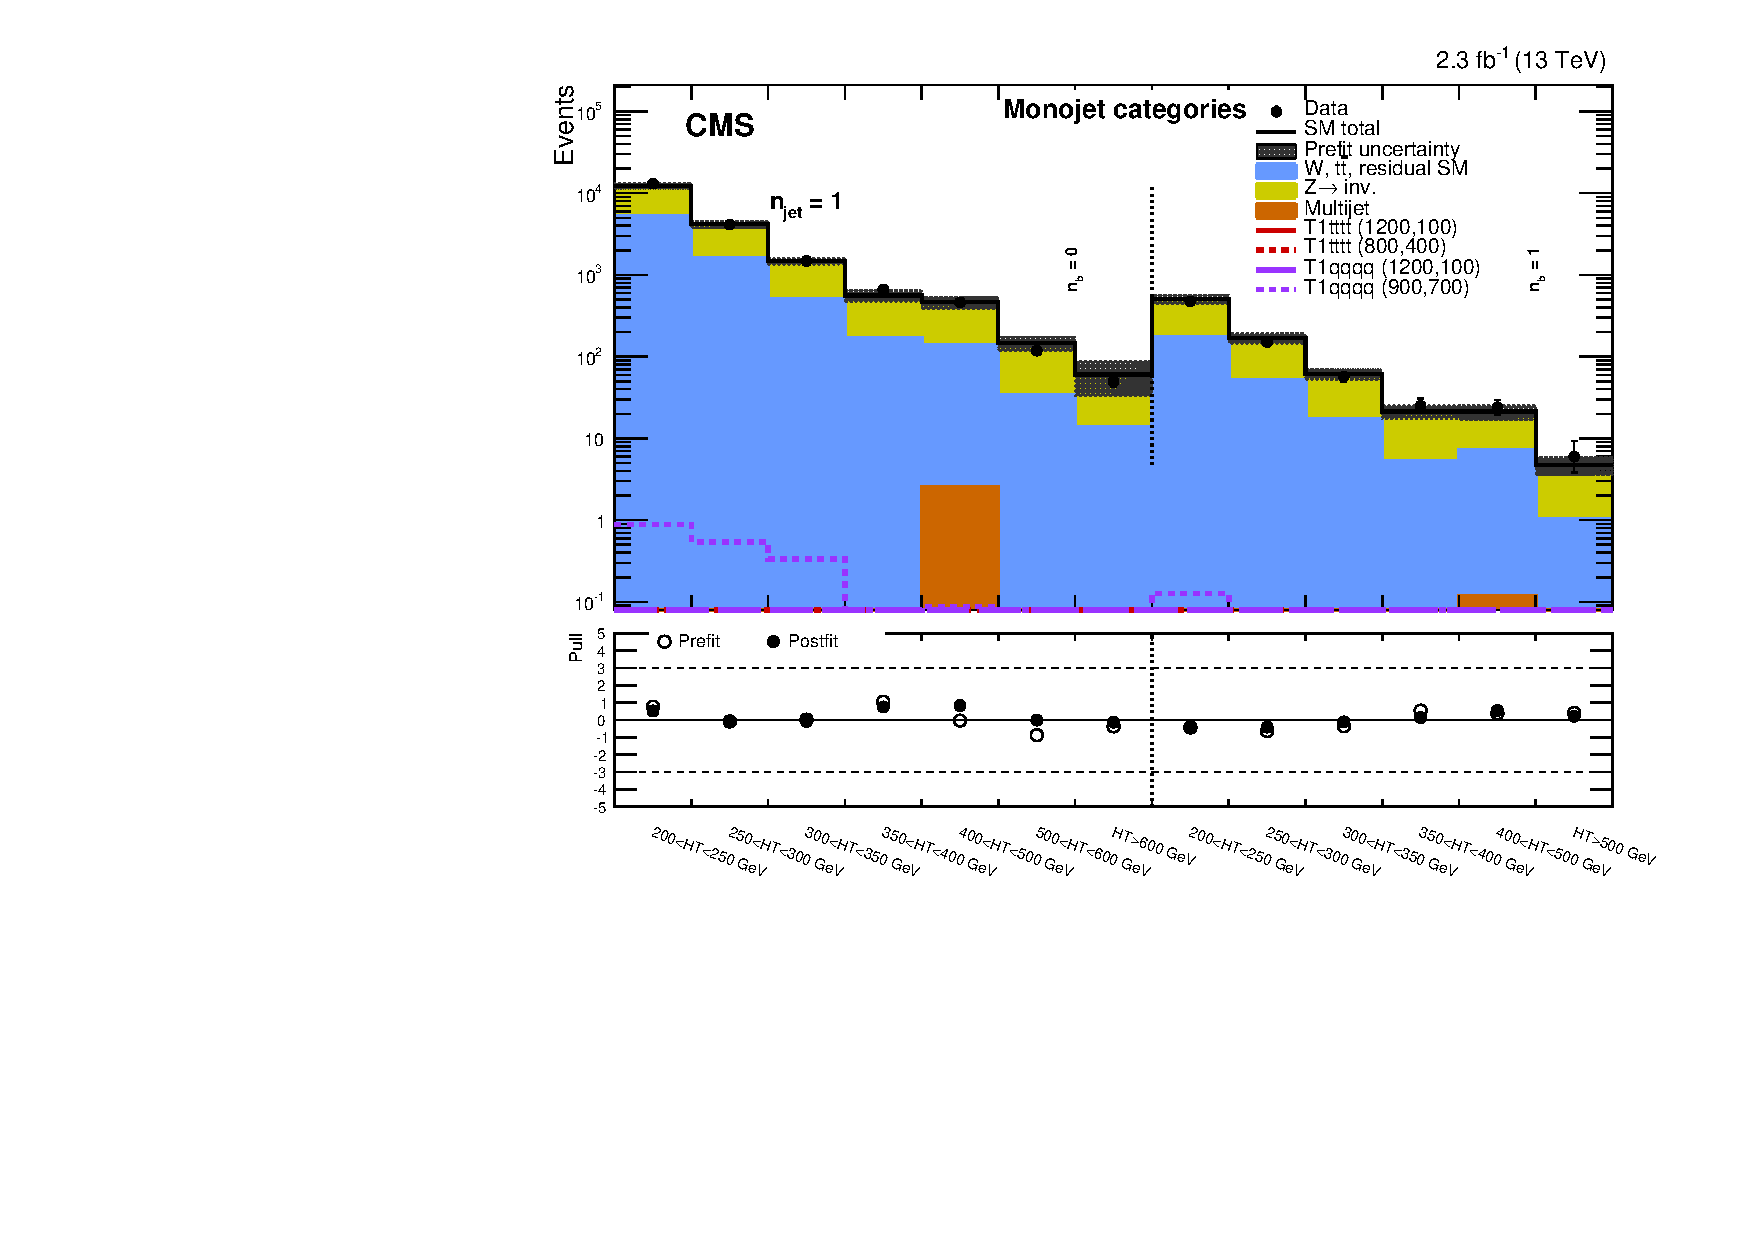
\includegraphics[width=0.8\linewidth]{figures/postFitResults/summaryPlots/summaryPlot_Monojet_prefit_overlay_fit_b}
    \end{figure}
  \end{center}
\end{landscape}

\clearpage
\begin{landscape}
  \begin{center}
    \begin{figure}[h!]
      \caption{Background yield predictions and data observation for the (\njet,\nb,\scalht) analysis bins (integrated over \MHT) in the asymmetric topologies. \label{fig:summaryPlot_Asymmetric}}.
      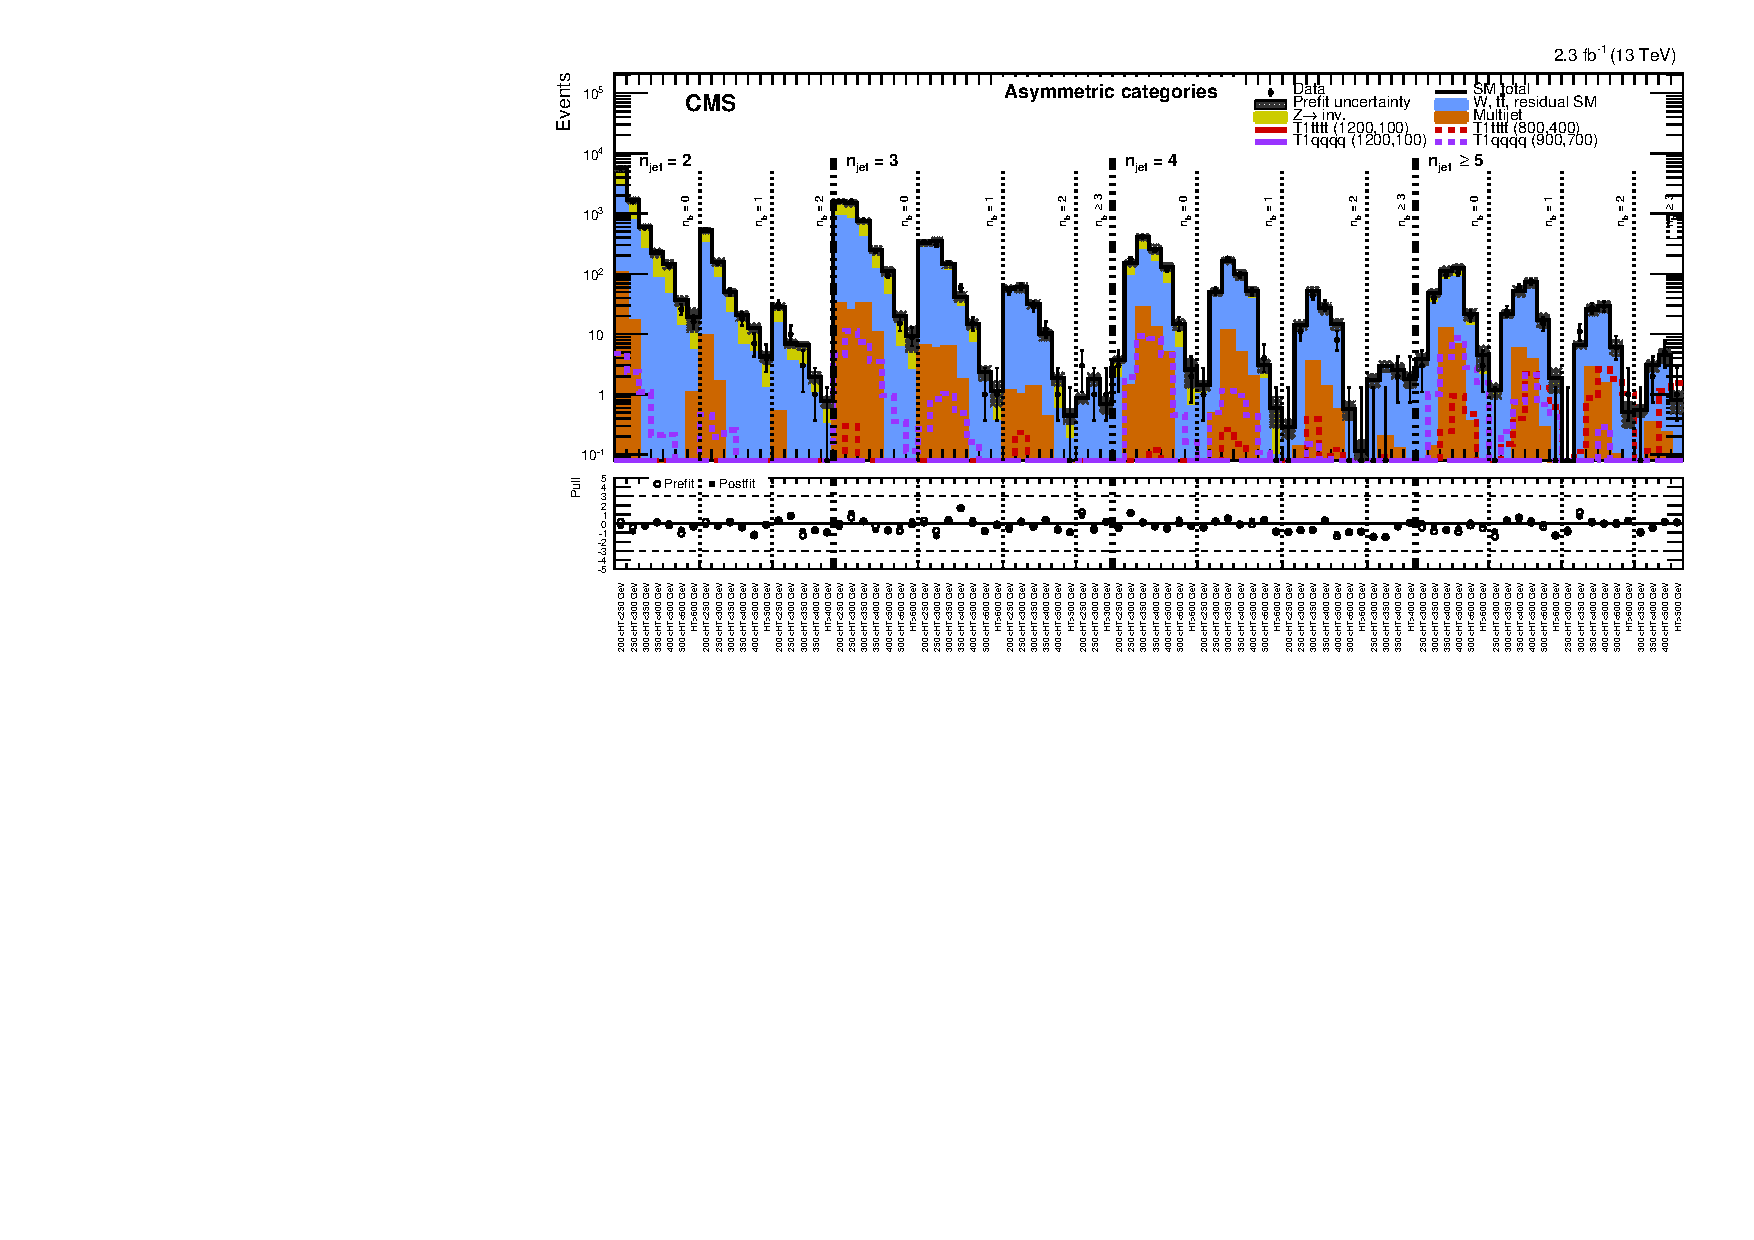
\includegraphics[width=0.9\linewidth]{figures/postFitResults/summaryPlots/summaryPlot_Asymmetric_prefit_overlay_fit_b}
    \end{figure}
  \end{center}
\end{landscape}

\clearpage
\begin{landscape}
  \begin{center}
    \begin{figure}[h!]
      \caption{Background yield predictions and data observation for the (\njet,\nb,\scalht) analysis bins (integrated over \MHT) in the symmetric topologies. \label{fig:summaryPlot_Symmetric}}.
      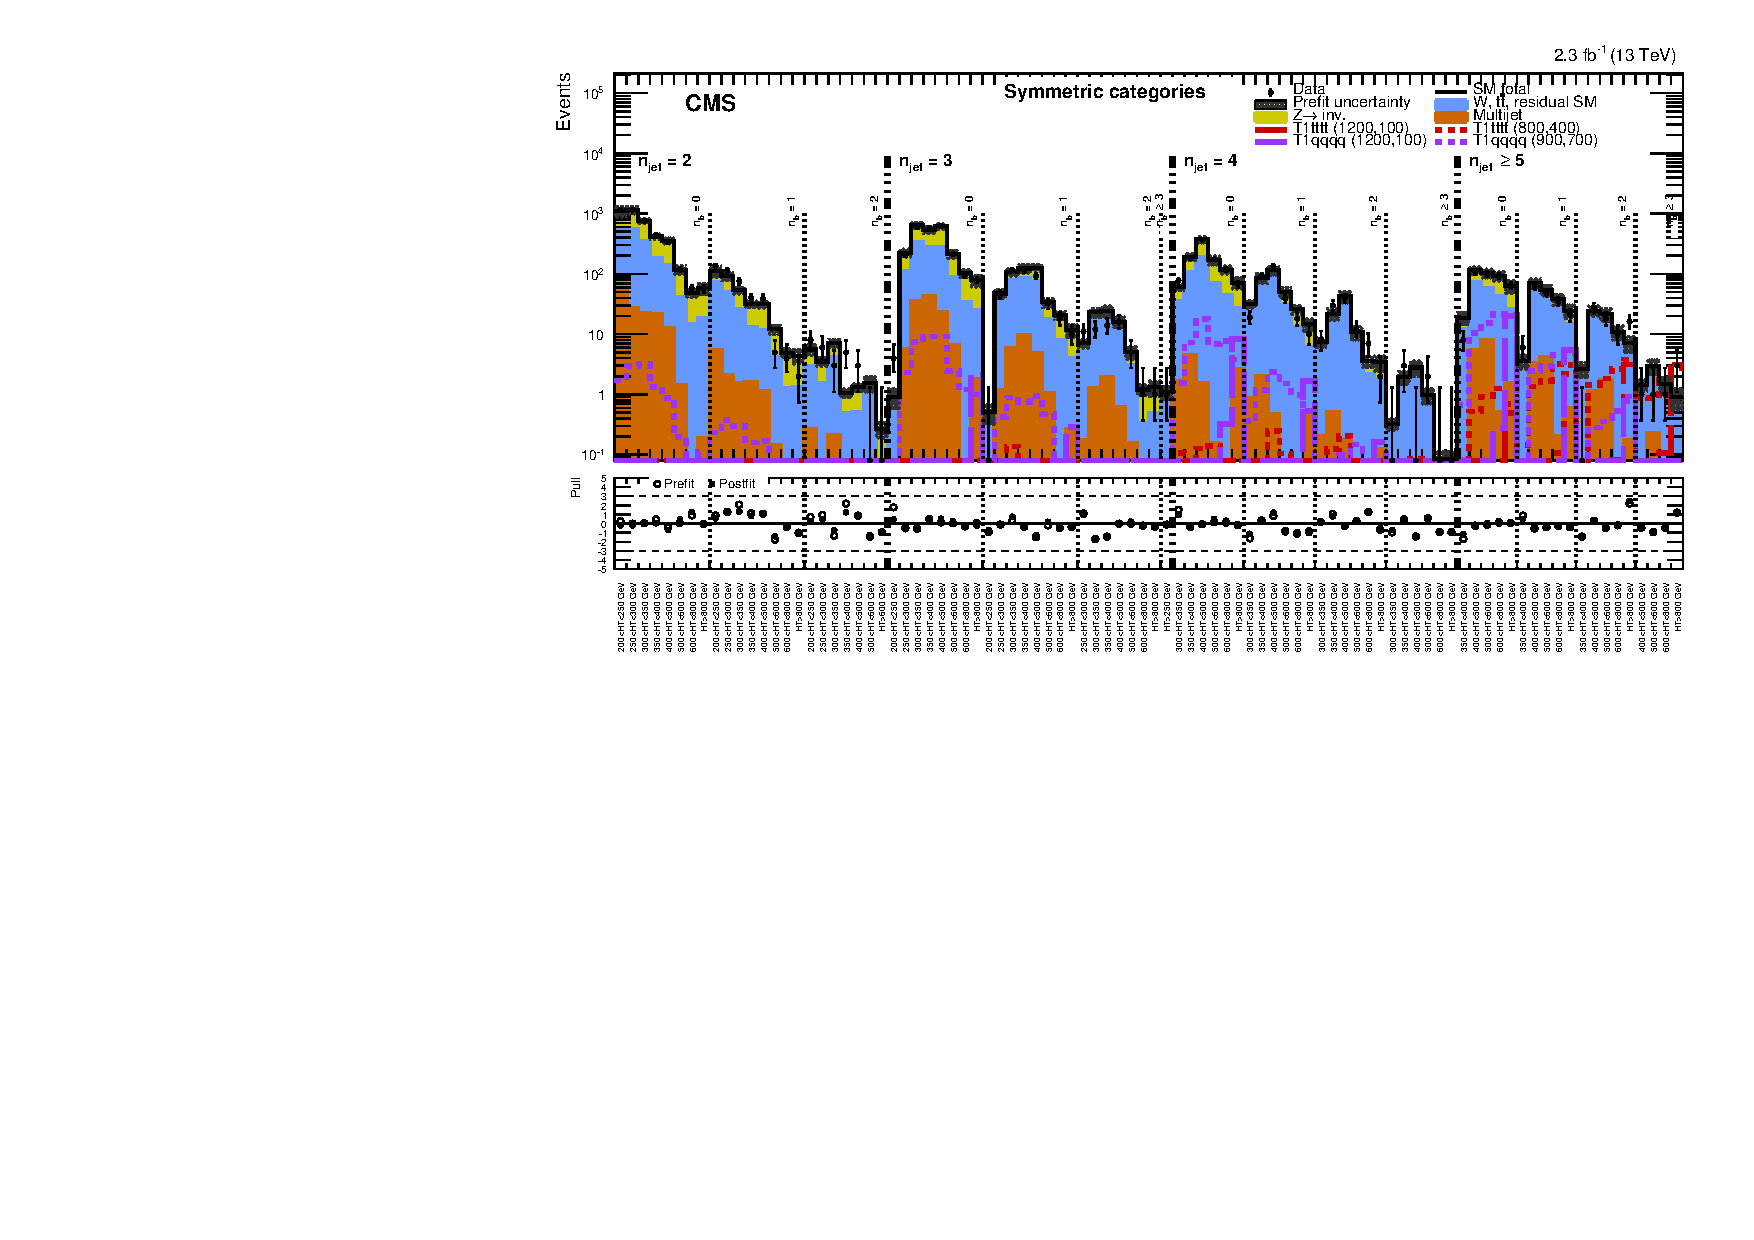
\includegraphics[width=0.9\linewidth]{figures/postFitResults/summaryPlots/summaryPlot_Symmetric_prefit_overlay_fit_b}
    \end{figure}
  \end{center}
\end{landscape}


\clearpage
  \begin{center}
    \begin{figure}[h!]
      \caption{Pulls of the observation compared to the prediction from the CR-only fit in the monojet categories (top-left), 
        asymmetric categories (top-right), symmetric categories (bottom-left) and all the categories combined (bottom-right). 
        The pulls are normalised to the total prediction uncertainty, including both the systematic and statistical component. \label{fig:pulls1D}}.
      \subfigure[Monojet categories]{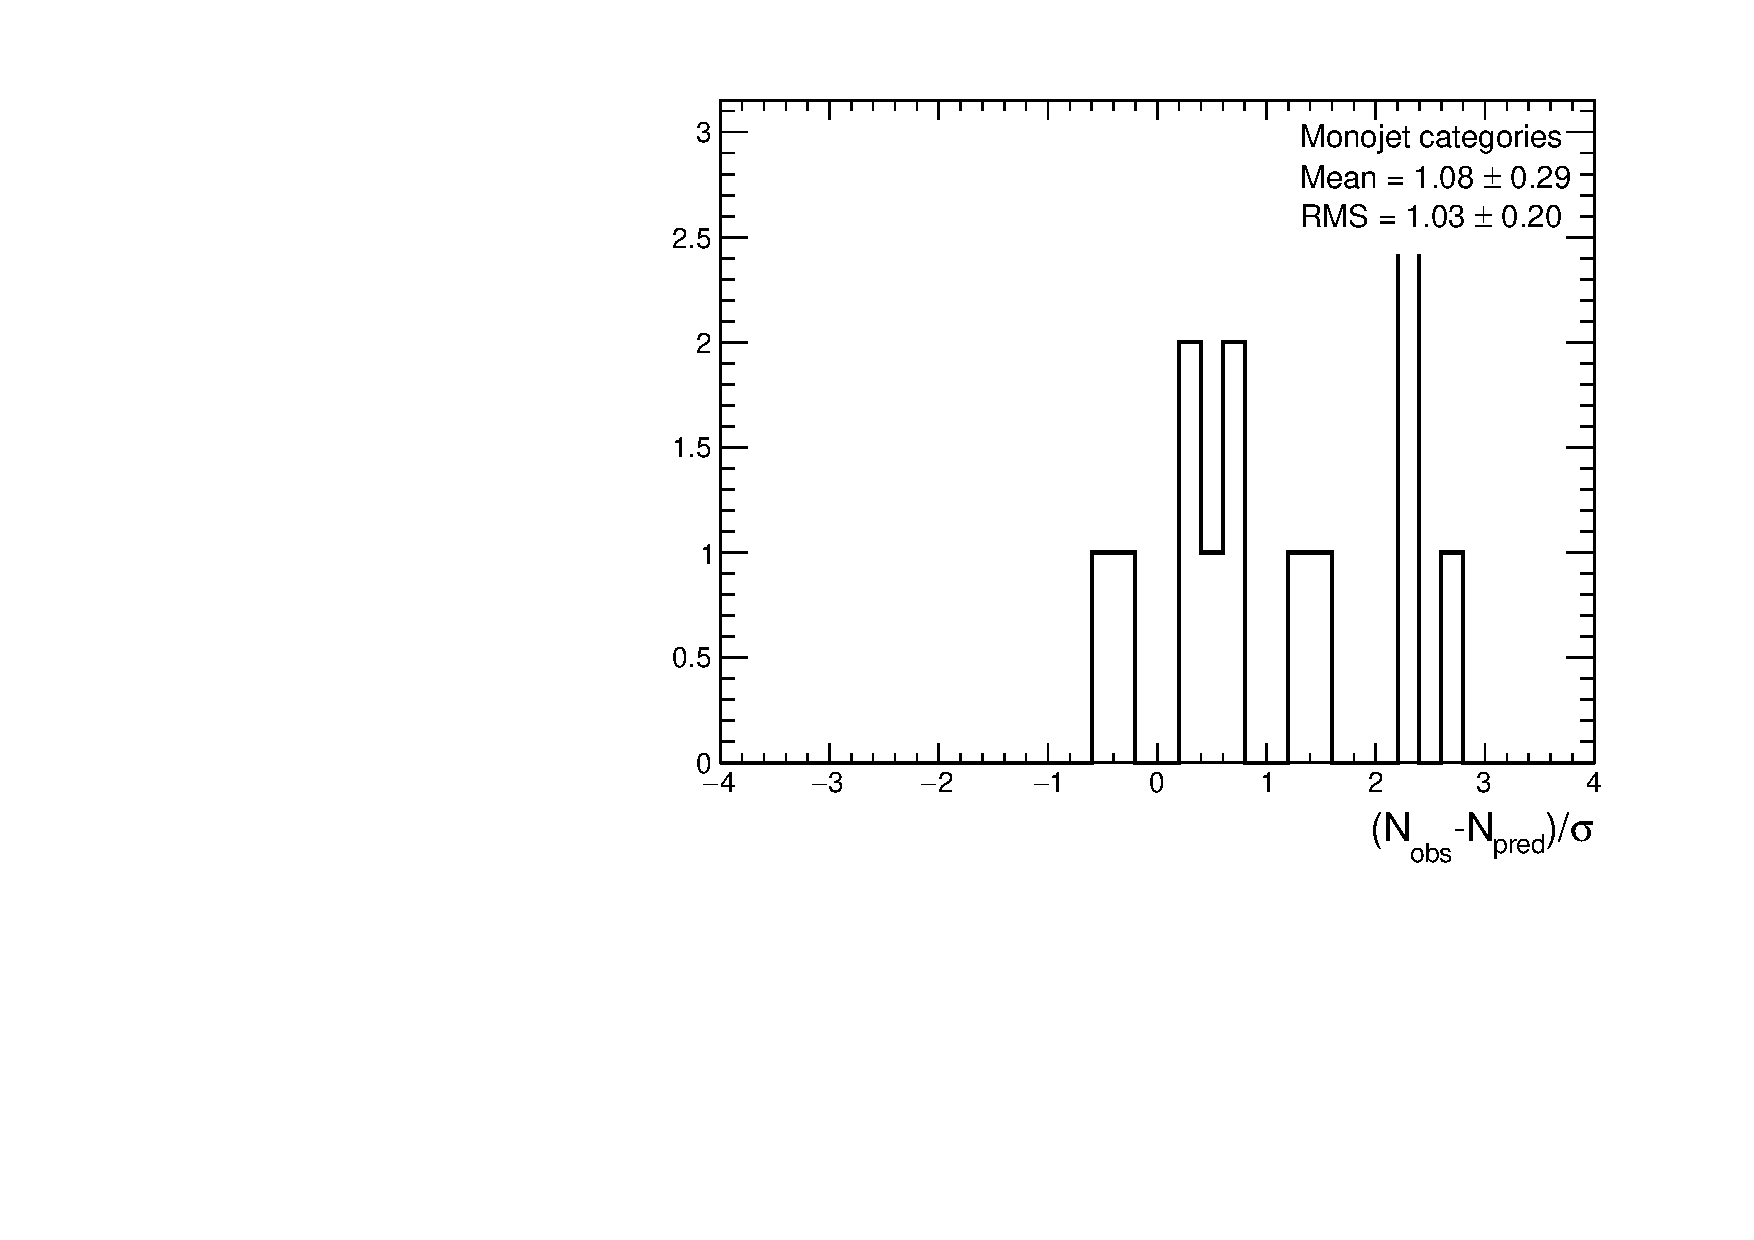
\includegraphics[width=0.45\linewidth]{figures/postFitResults/summaryPlots/pulls_Monojet_prefit}} 
      \subfigure[Asymmetric categories]{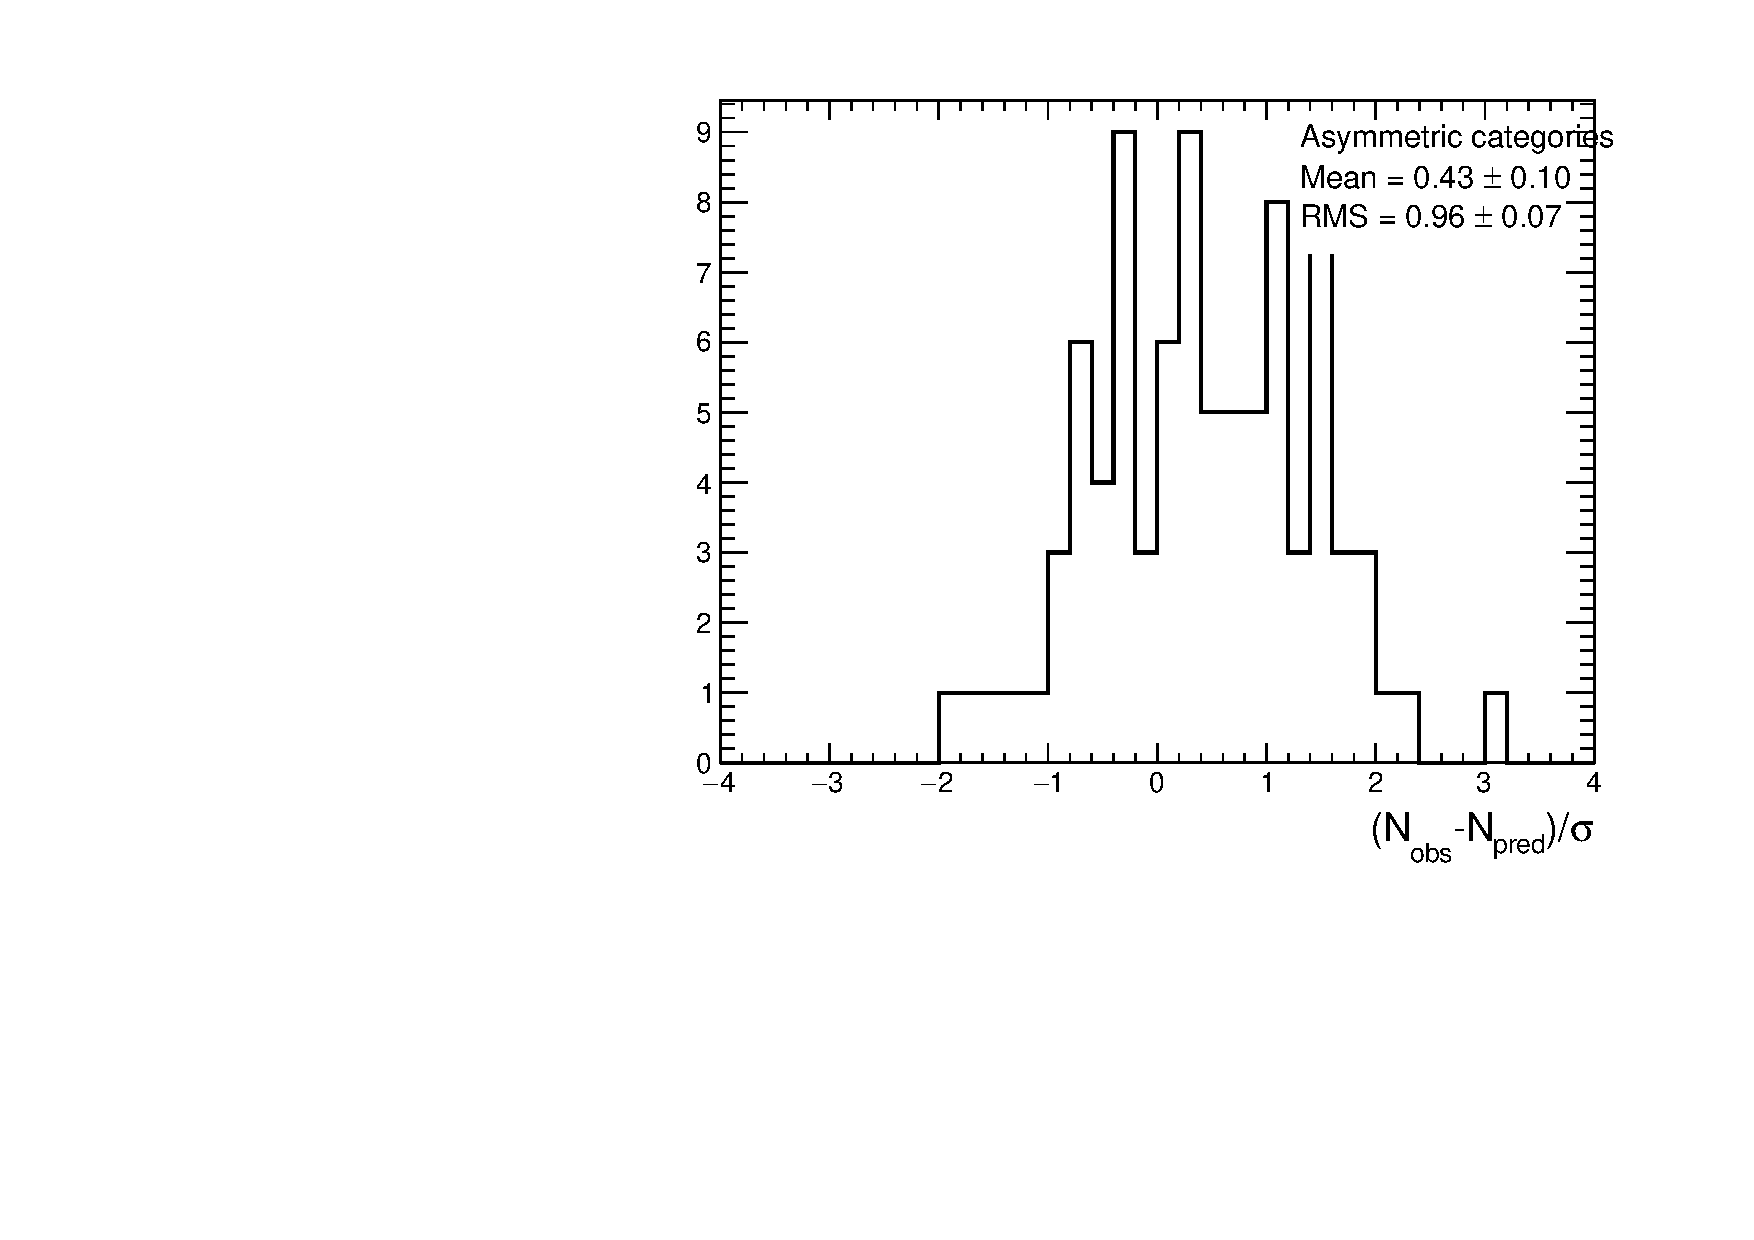
\includegraphics[width=0.45\linewidth]{figures/postFitResults/summaryPlots/pulls_Asymmetric_prefit}} \\
      \subfigure[Symmetric categories]{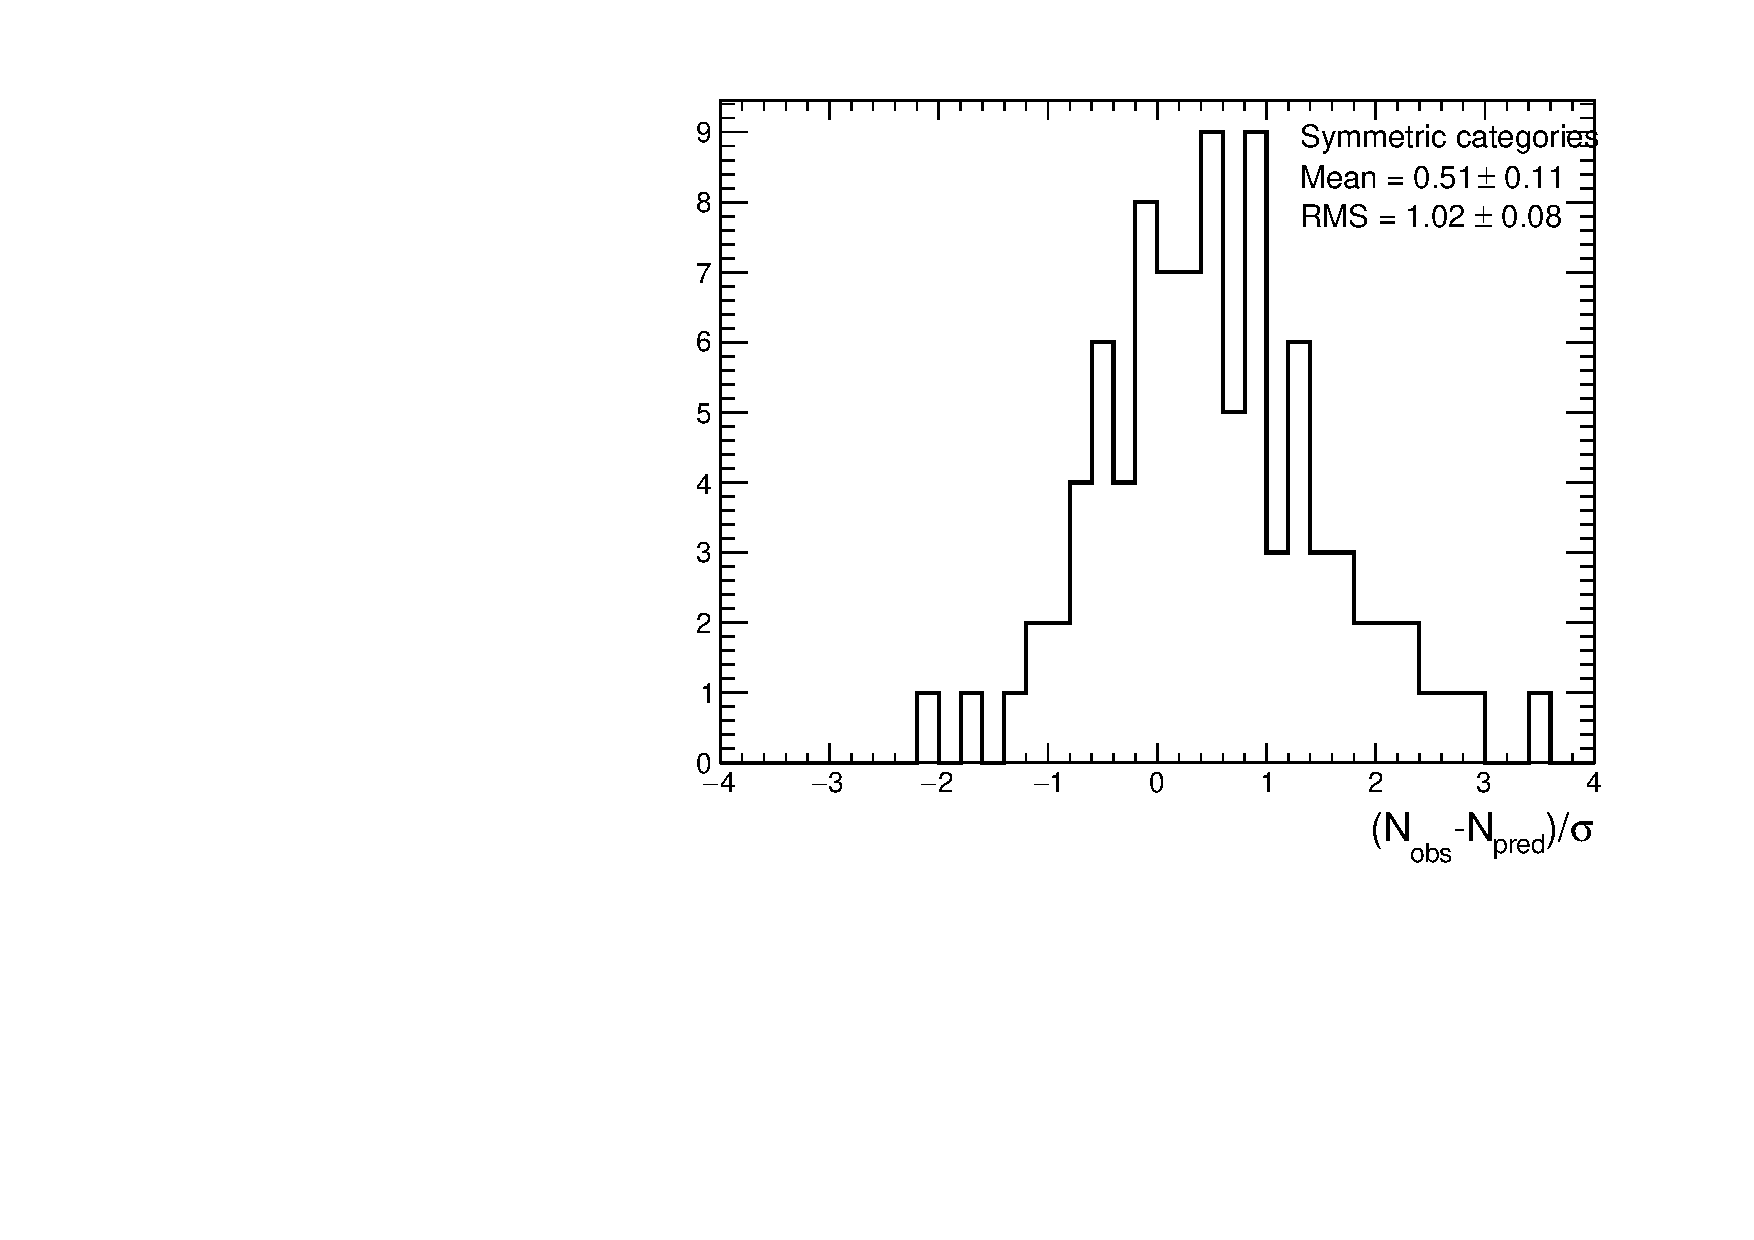
\includegraphics[width=0.45\linewidth]{figures/postFitResults/summaryPlots/pulls_Symmetric_prefit}} 
      \subfigure[All categories]{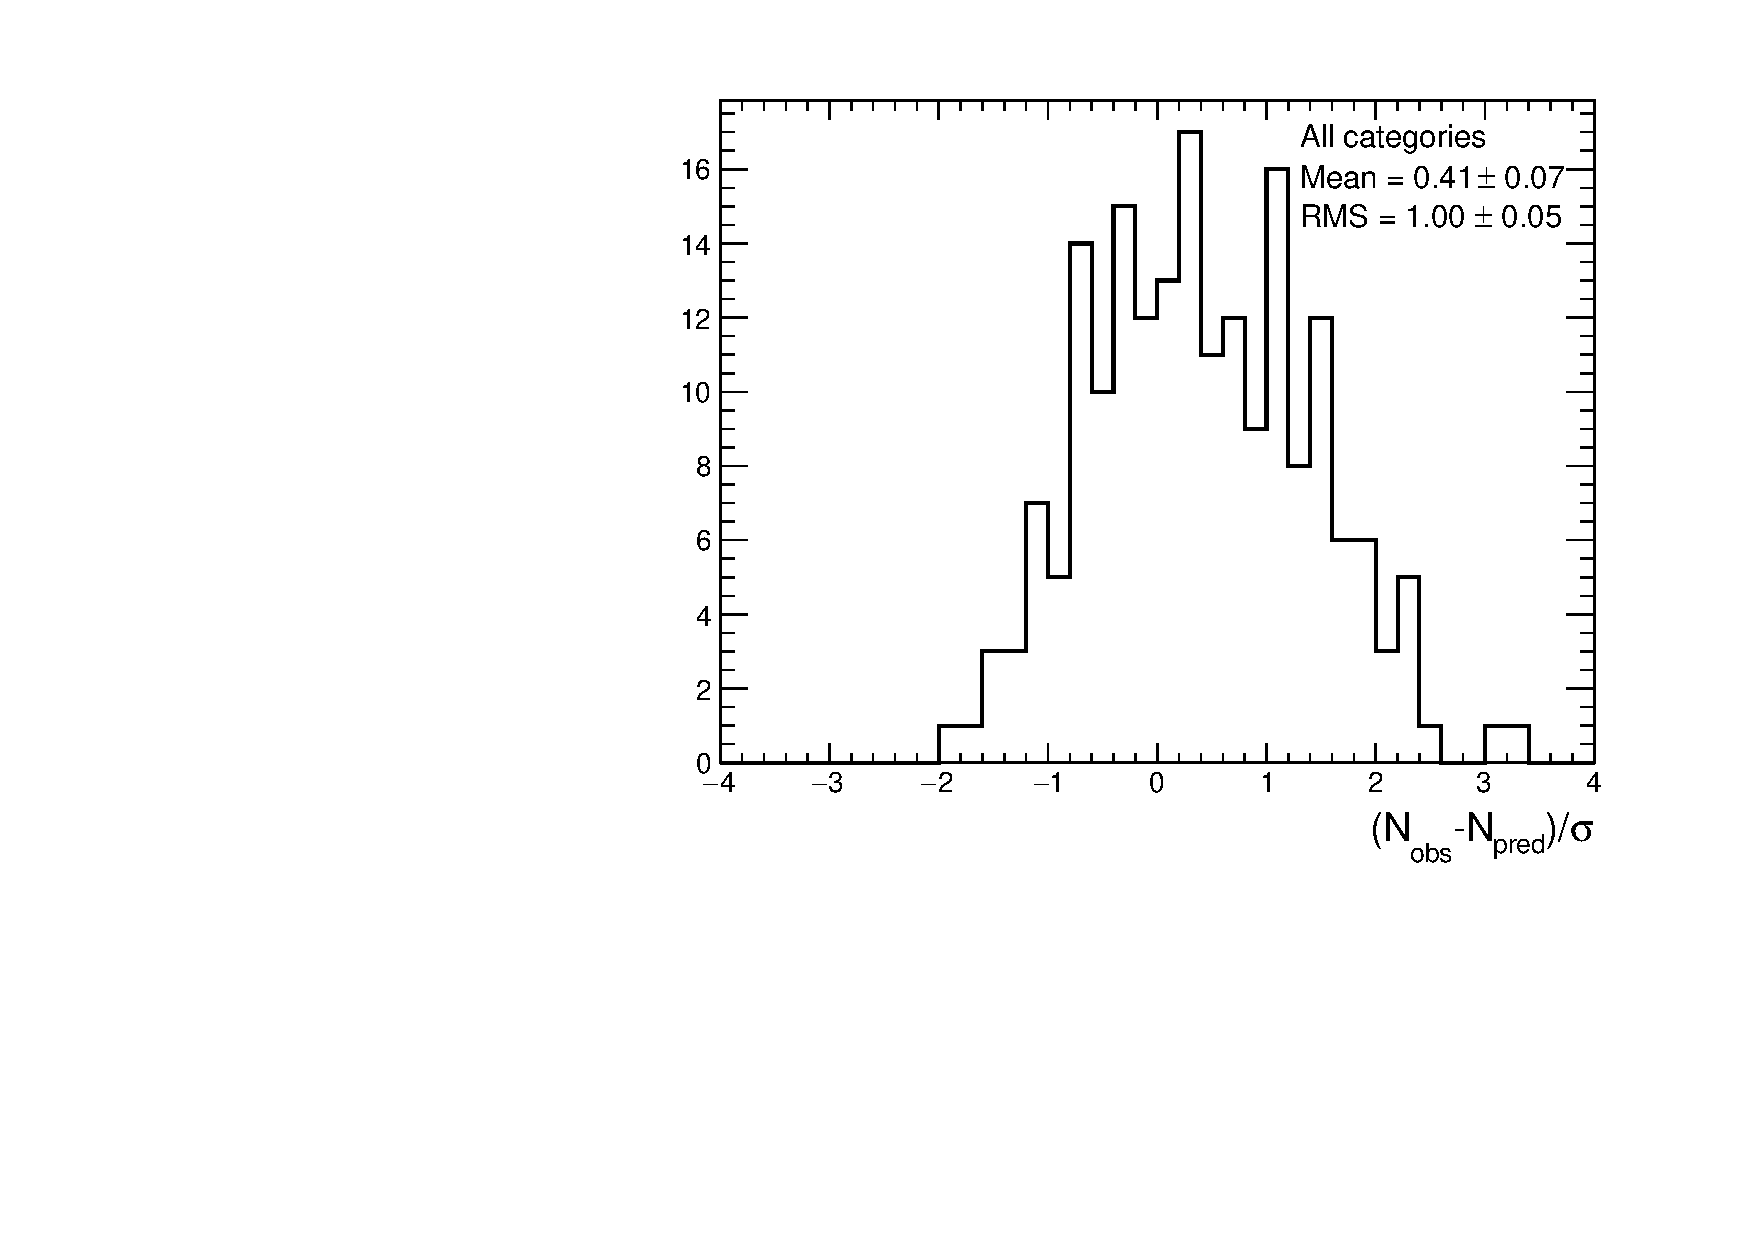
\includegraphics[width=0.45\linewidth]{figures/postFitResults/summaryPlots/pulls_all_prefit}} \\
    \end{figure}
  \end{center}


\clearpage
\begin{figure}[tbhp]
    \caption{\mht templates for some (\njet,\nb,\scalht) analysis bins, for the asymmetric topologies. \label{fig:mht-templates-asym} }
  \begin{center}
    \subfigure[$\njet = 4a$, $\nb = 0$, $350 < \scalht < 400$ GeV]{ 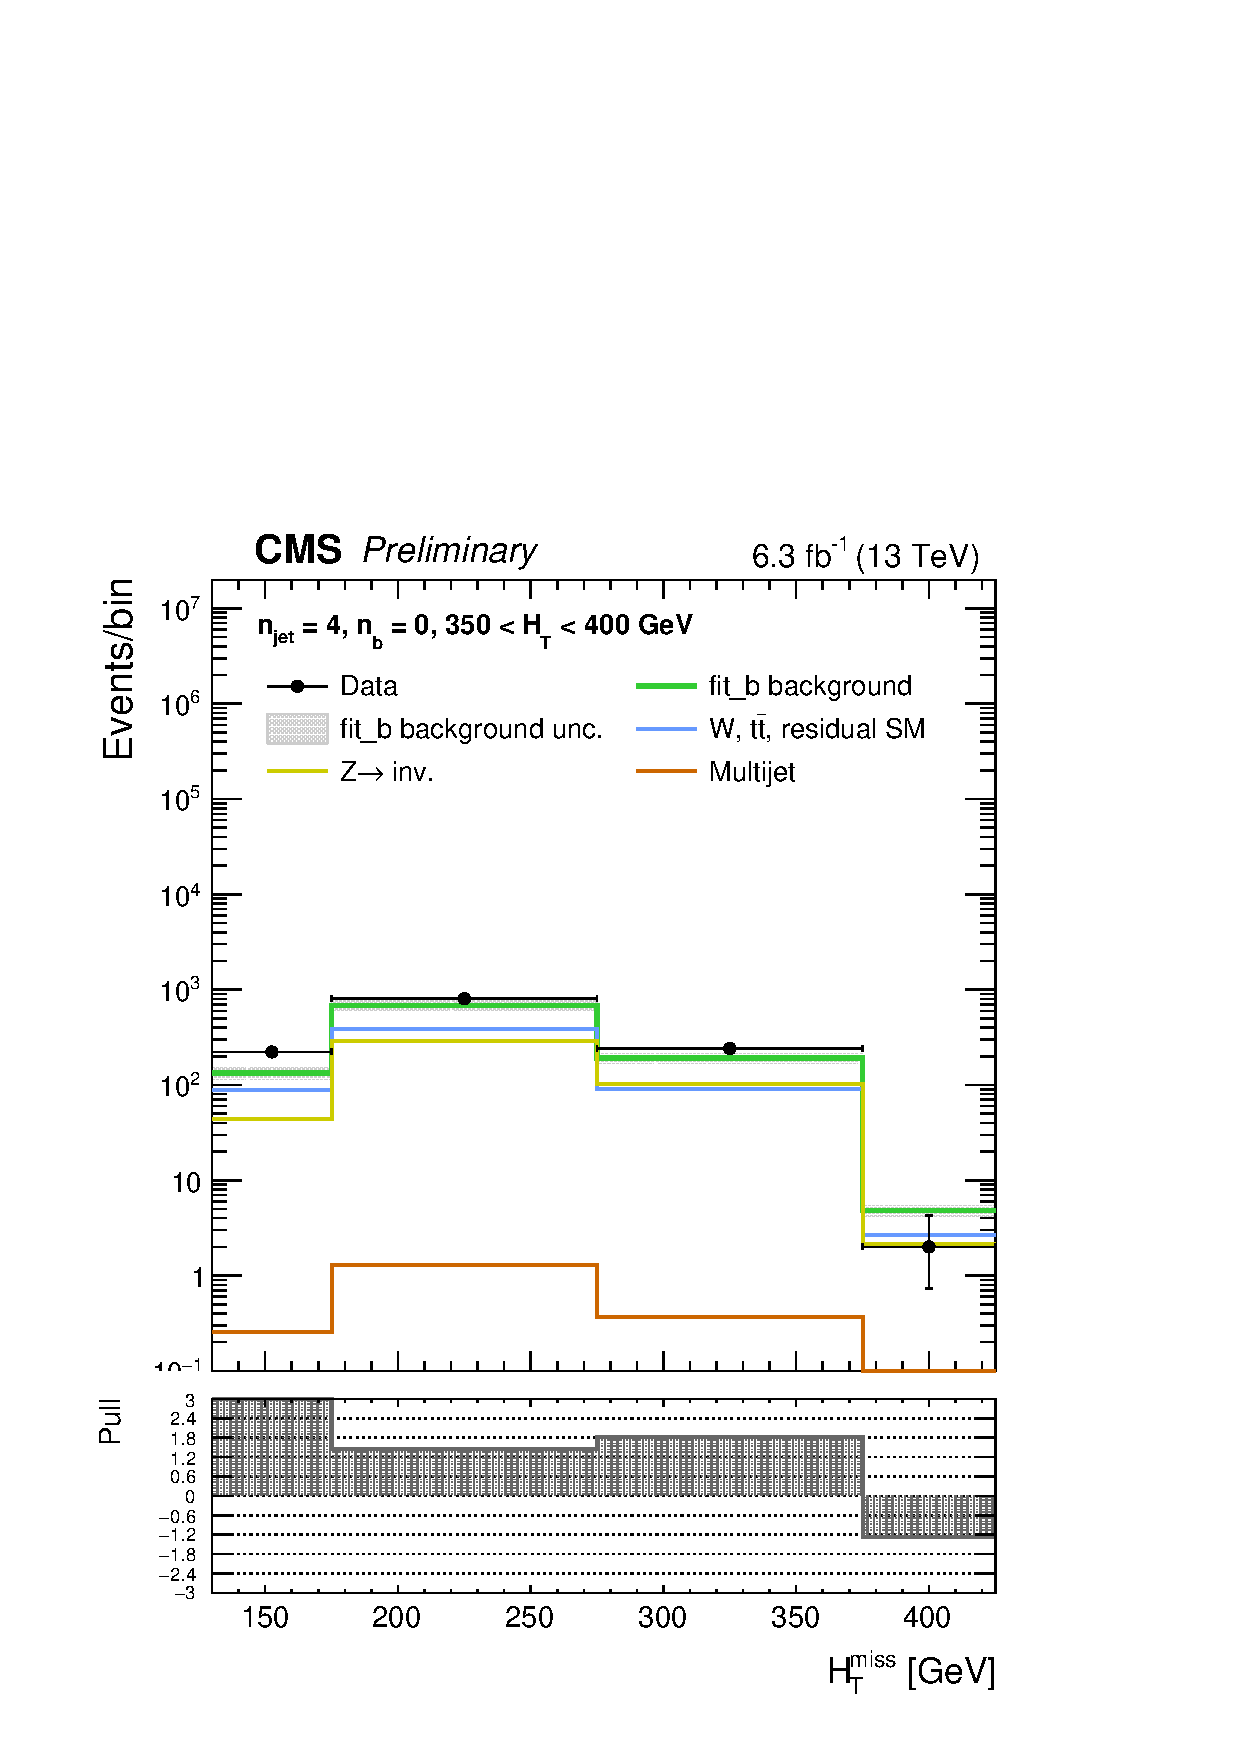
\includegraphics[width=0.45\textwidth]{figures/postFitResults/shapePlots/mhtShape_eq0b_eq4a_350_400_fit_b} } ~~
    \subfigure[$\njet = 3a$, $\nb = 0$, $400 < \scalht < 500$ GeV]{ 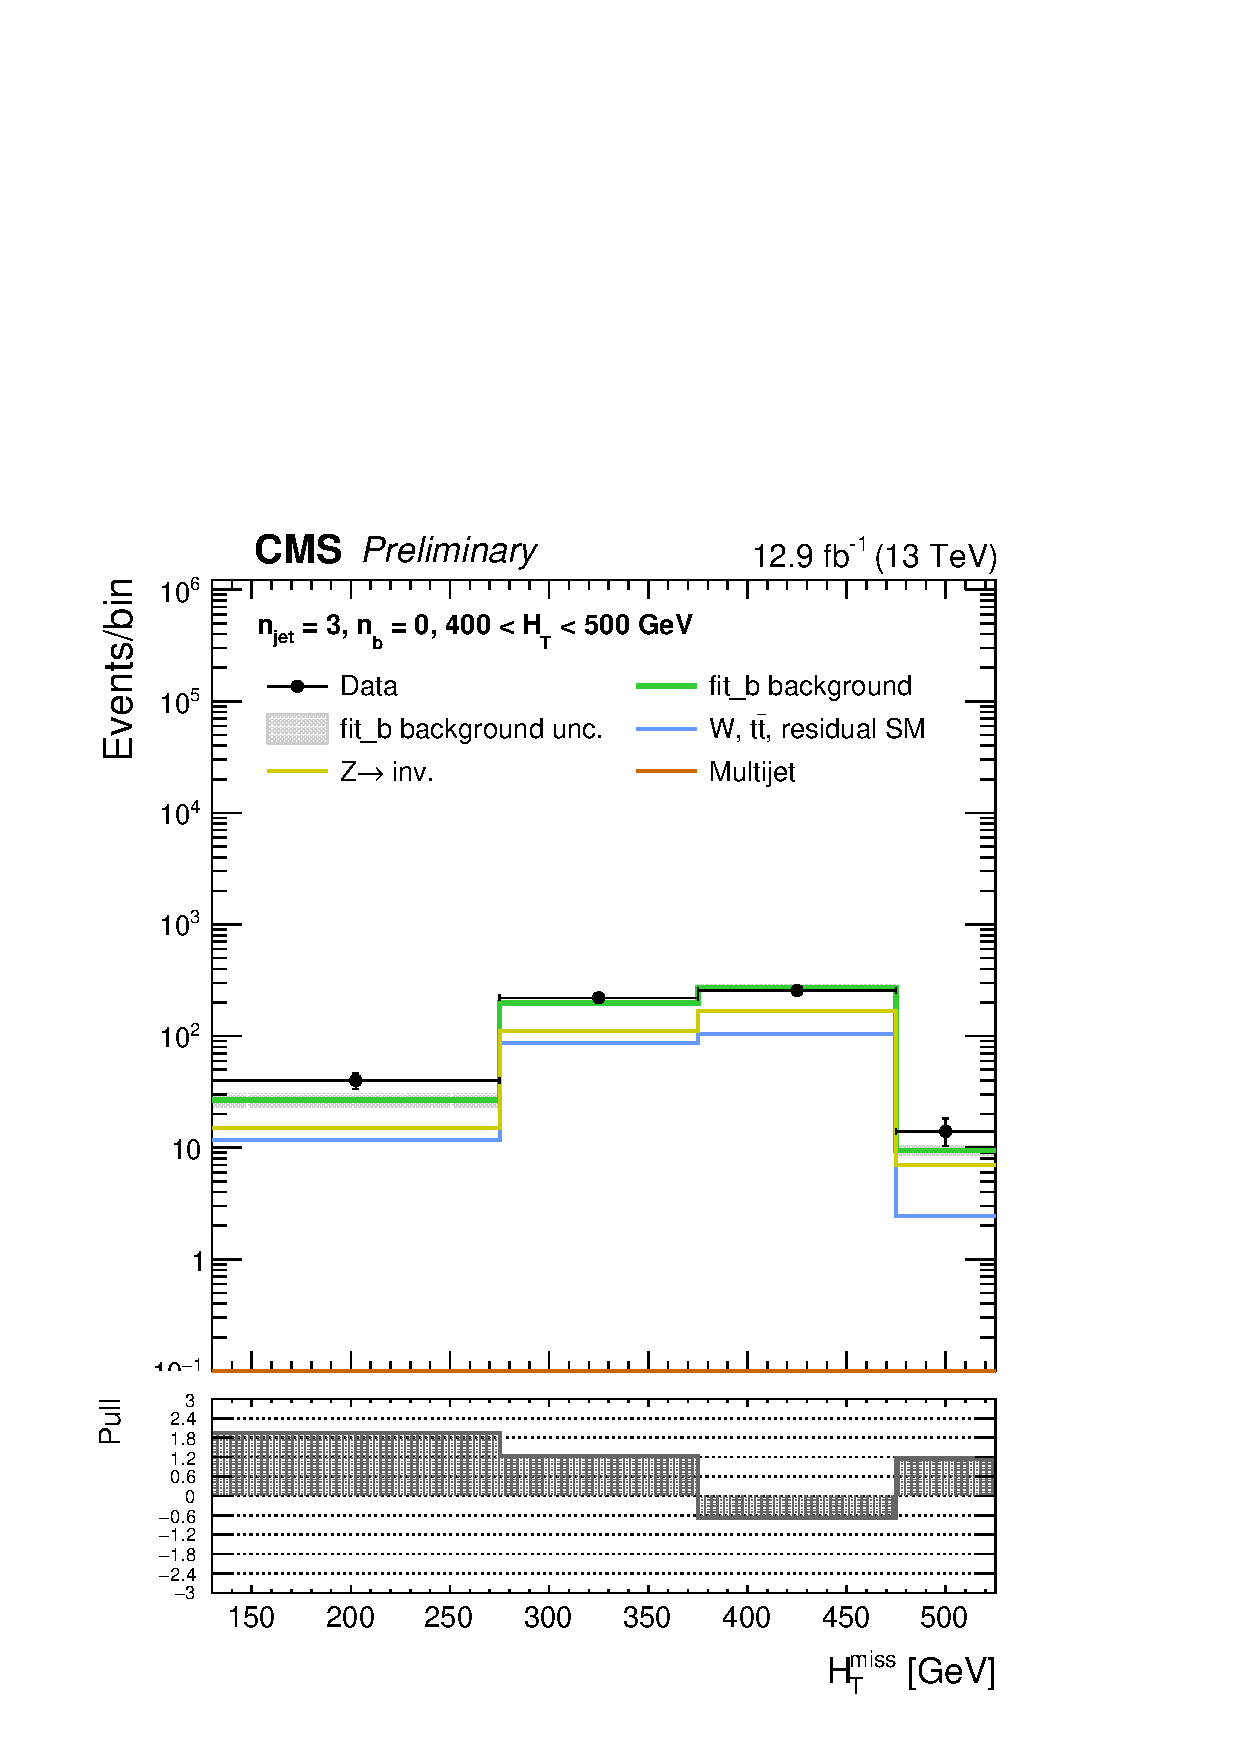
\includegraphics[width=0.45\textwidth]{figures/postFitResults/shapePlots/mhtShape_eq0b_eq3a_400_500_fit_b} } \\
    \subfigure[$\njet = 3a$, $\nb = 1$, $300 < \scalht < 350$ GeV]   { 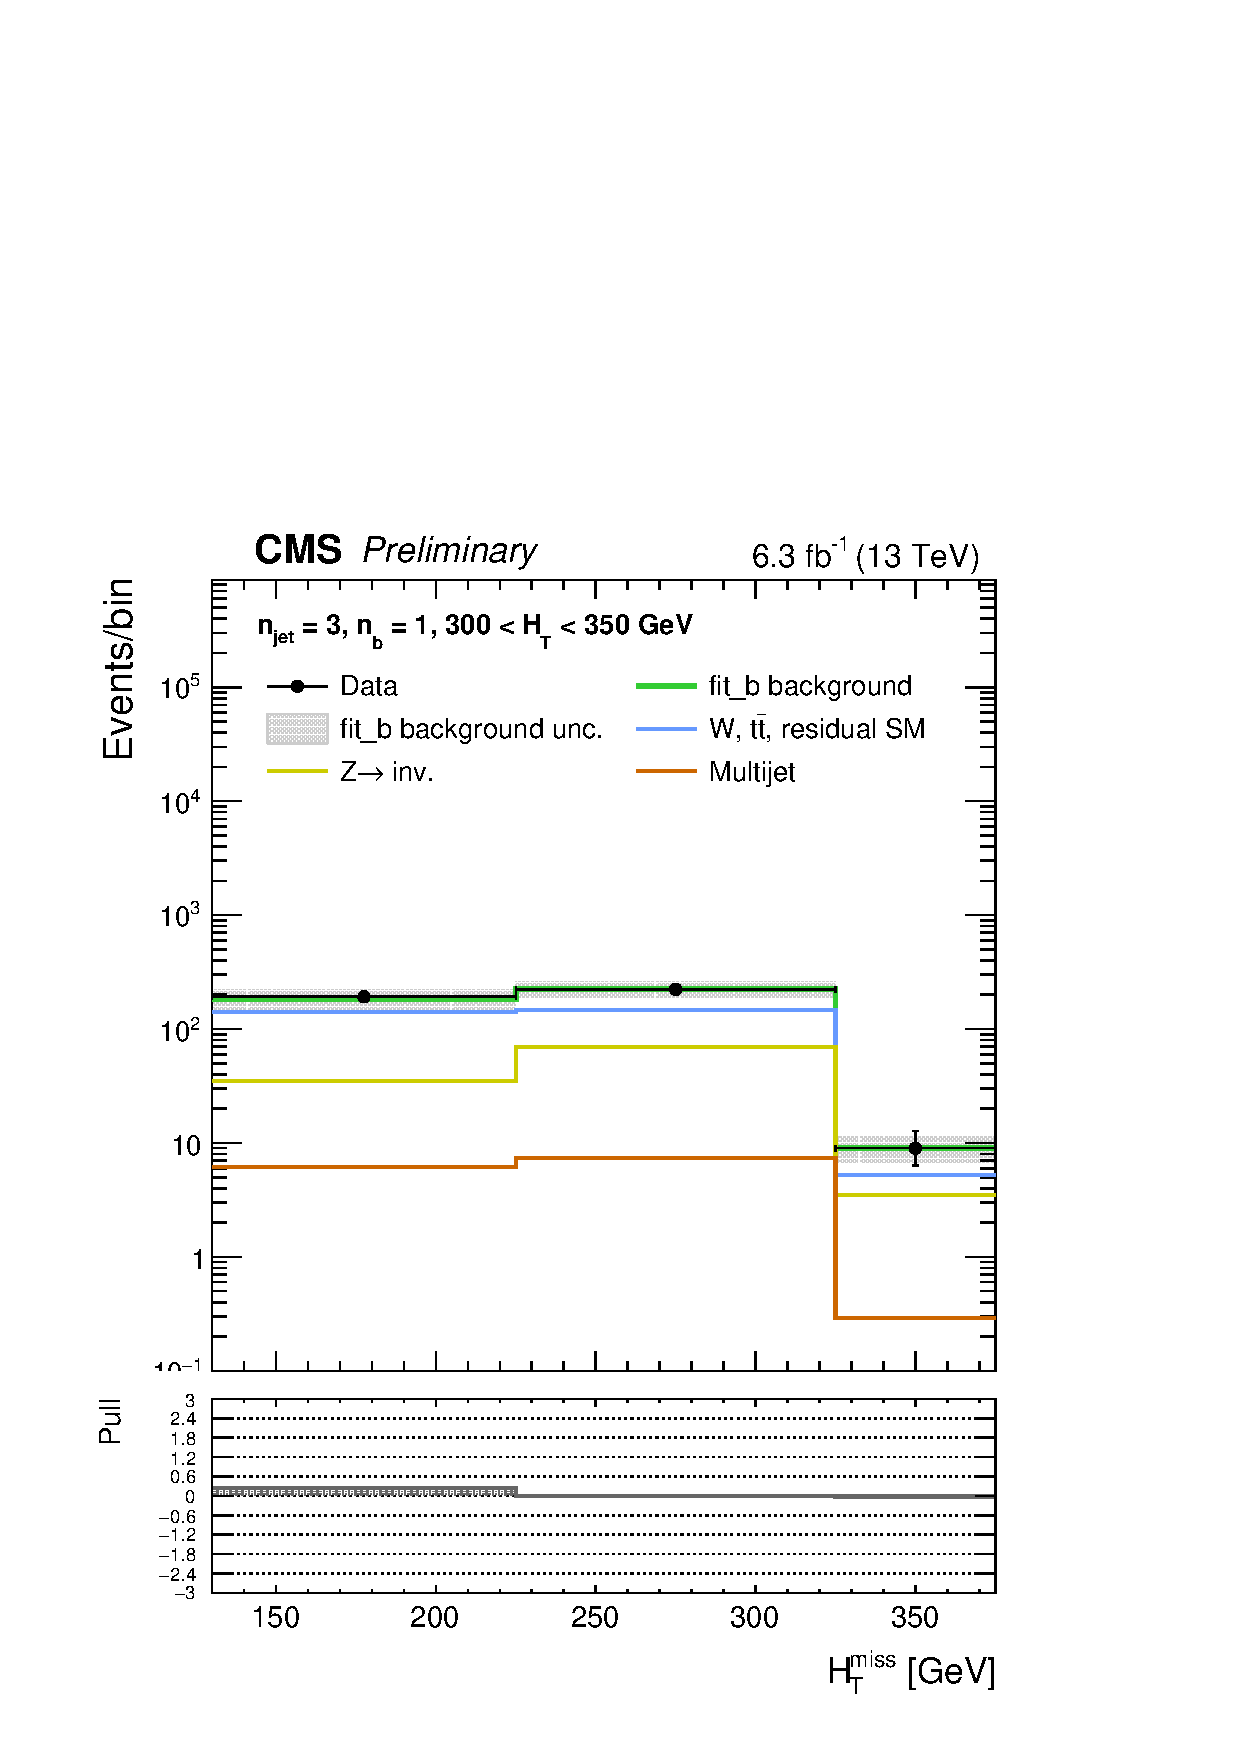
\includegraphics[width=0.45\textwidth]{figures/postFitResults/shapePlots/mhtShape_eq1b_eq3a_300_350_fit_b} } ~~
    \subfigure[$\njet \geq 5a$, $\nb = 2$, $400 < \scalht < 500$ GeV]{ 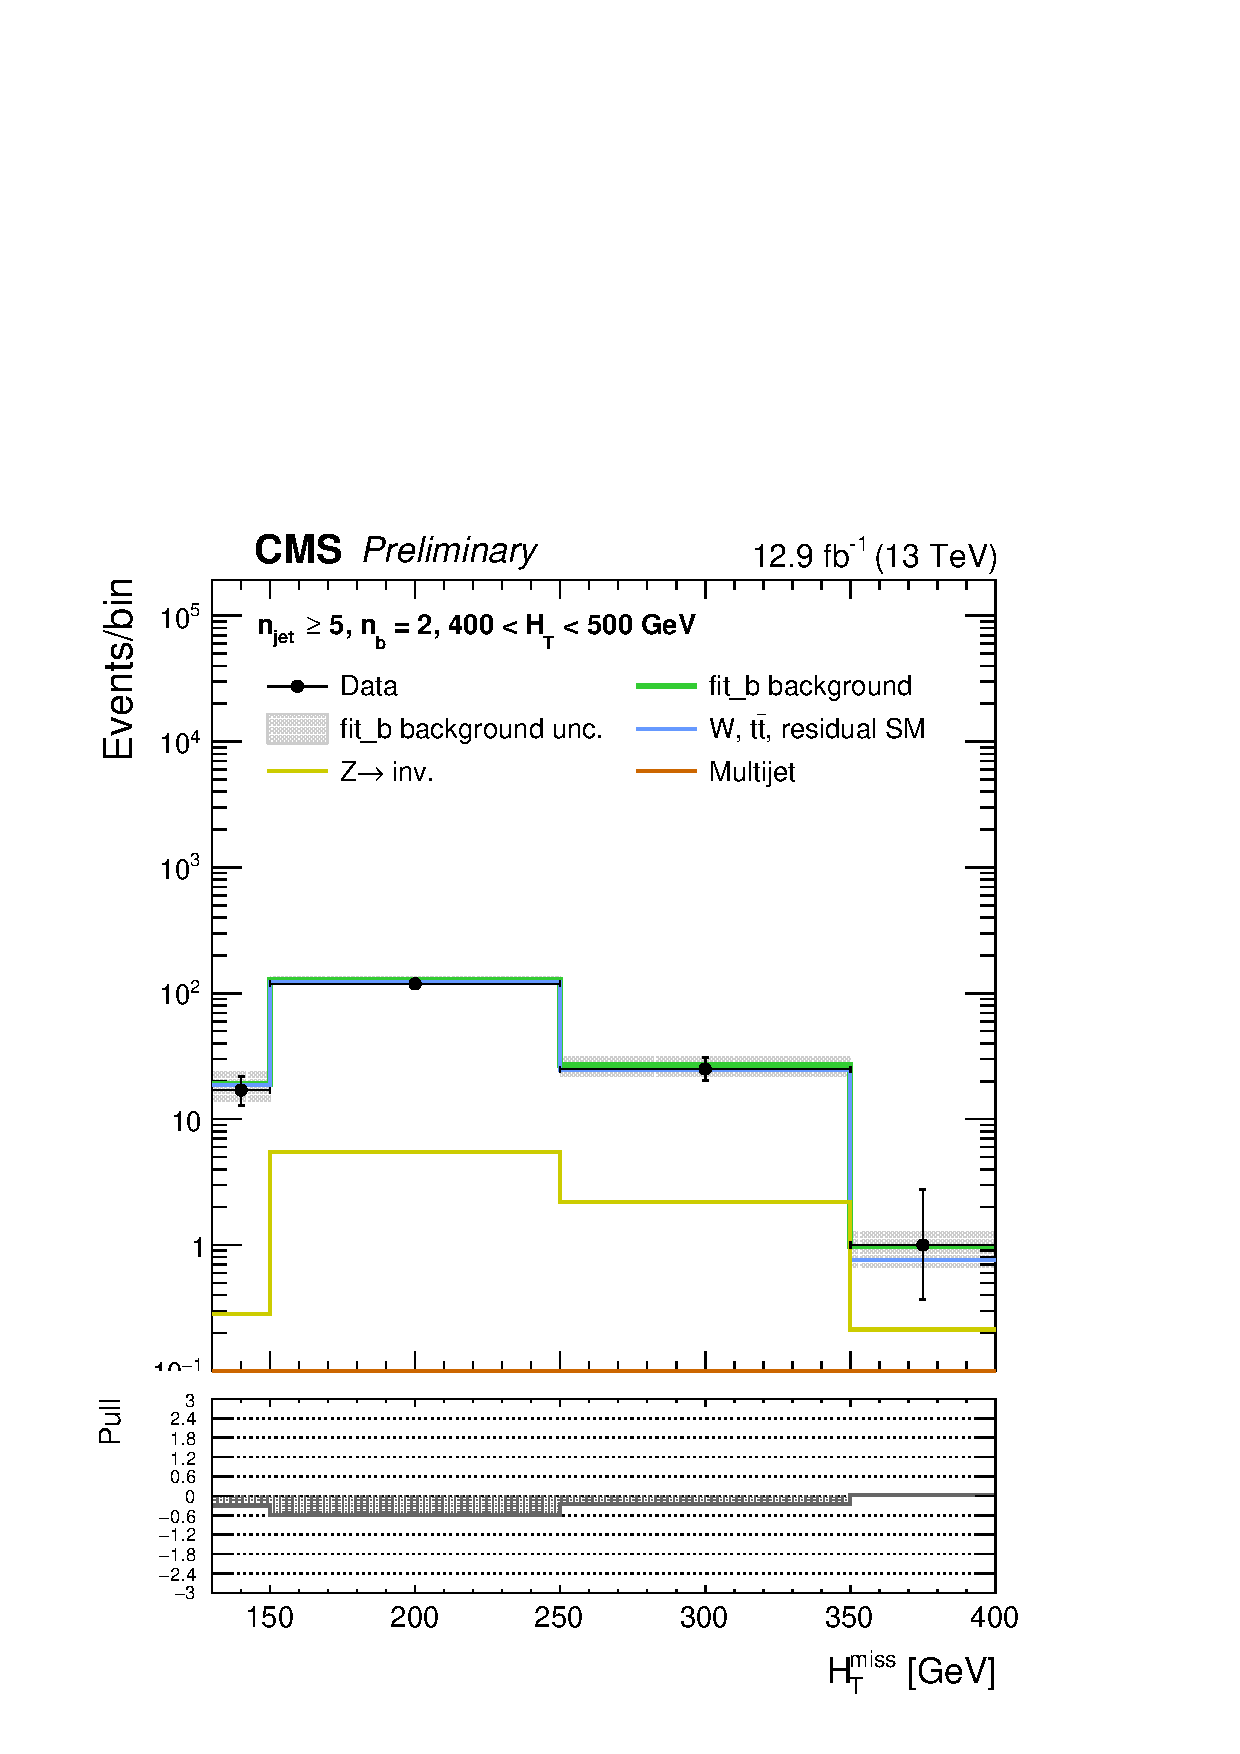
\includegraphics[width=0.45\textwidth]{figures/postFitResults/shapePlots/mhtShape_eq2b_ge5a_400_500_fit_b} } \\
  \end{center}
\end{figure}

\clearpage
\begin{figure}[tbhp]
    \caption{ \mht templates for some (\njet,\nb,\scalht) analysis bins, for the symmetric topologies. \label{fig:mht-templates-sym} }
  \begin{center}
    \subfigure[$\njet = \geq 5$, $\nb = 0$, $500 < \scalht < 600$ GeV]{ 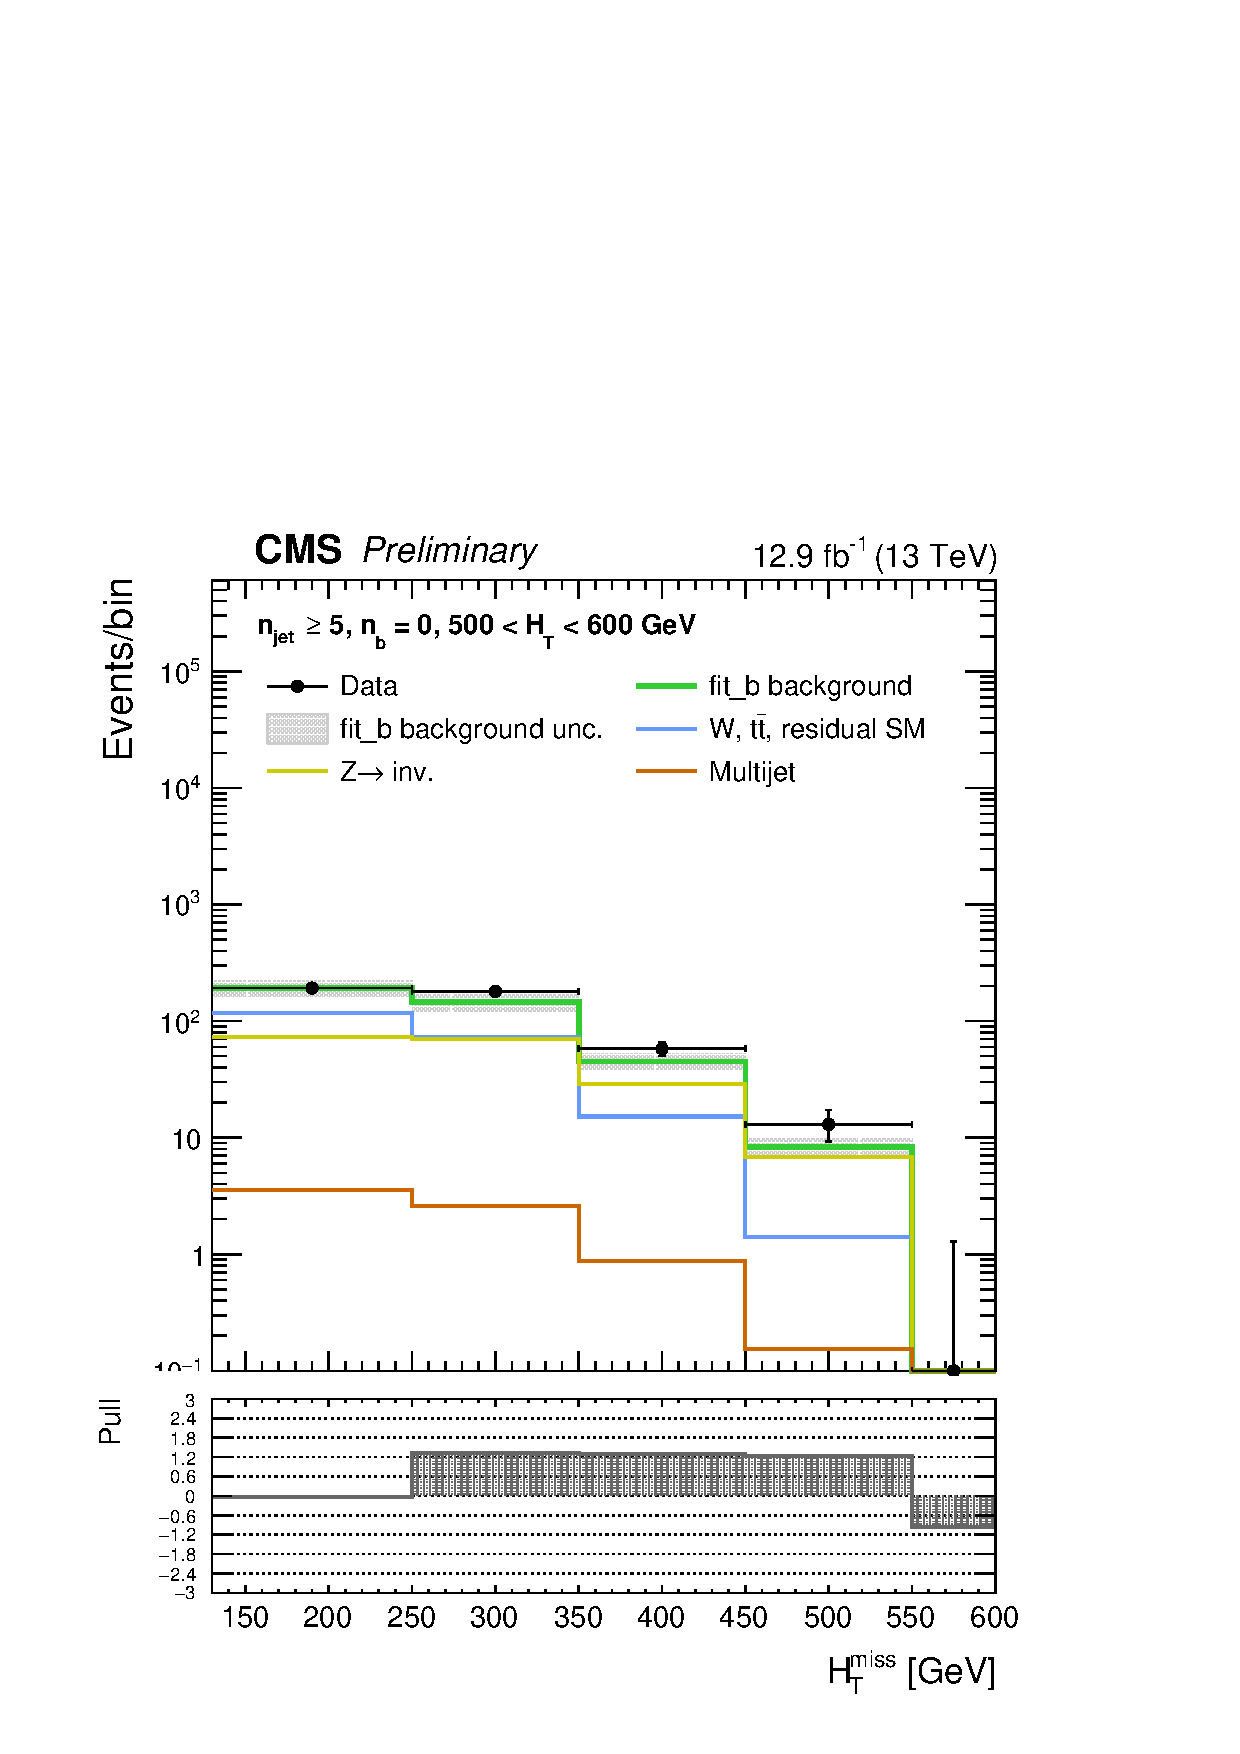
\includegraphics[width=0.45\textwidth]{figures/postFitResults/shapePlots/mhtShape_eq0b_ge5j_500_600_fit_b} } ~~
    \subfigure[$\njet = \geq 5$, $\nb = 2$, $500 < \scalht < 600$ GeV]{ 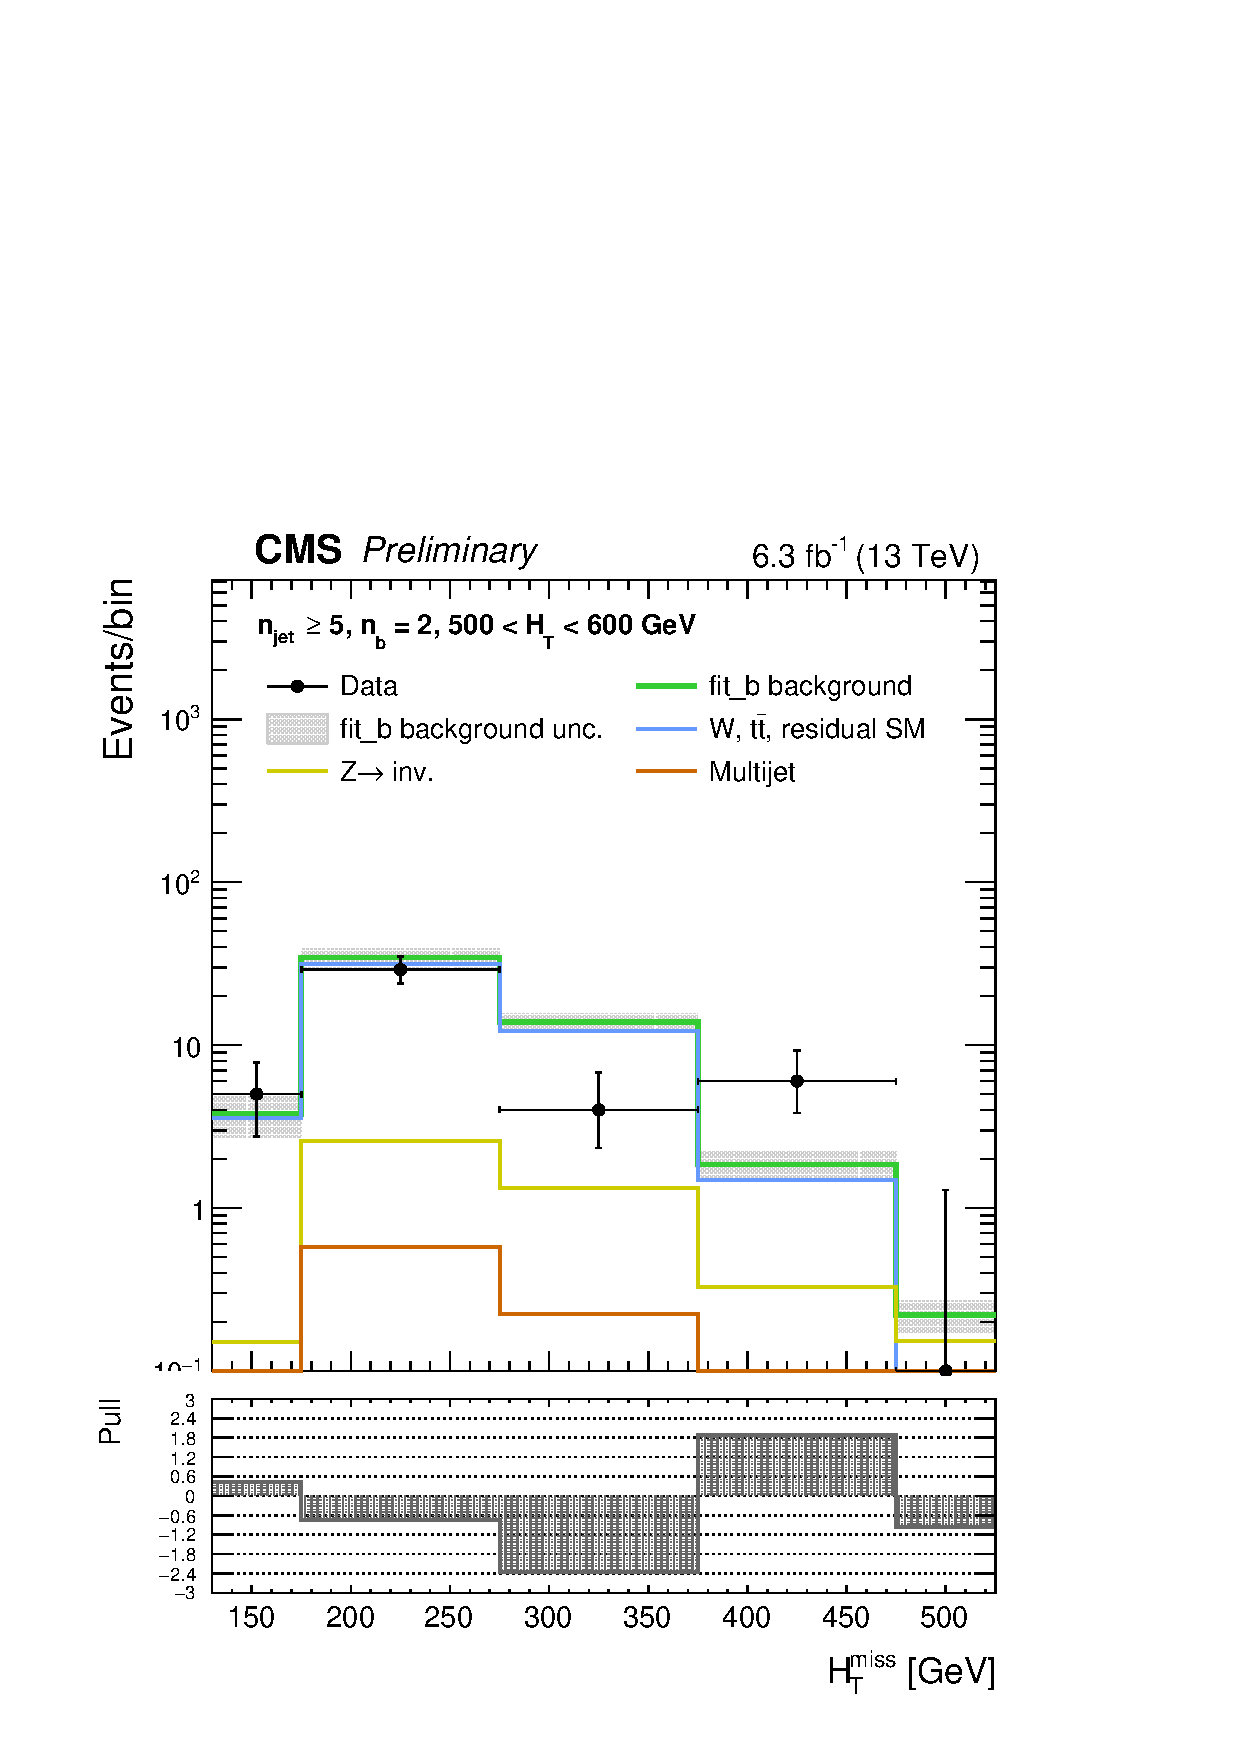
\includegraphics[width=0.45\textwidth]{figures/postFitResults/shapePlots/mhtShape_eq2b_ge5j_500_600_fit_b} } \\
    \subfigure[$\njet = \geq 5$, $\nb = 0$, $\scalht > 800$ GeV]   { 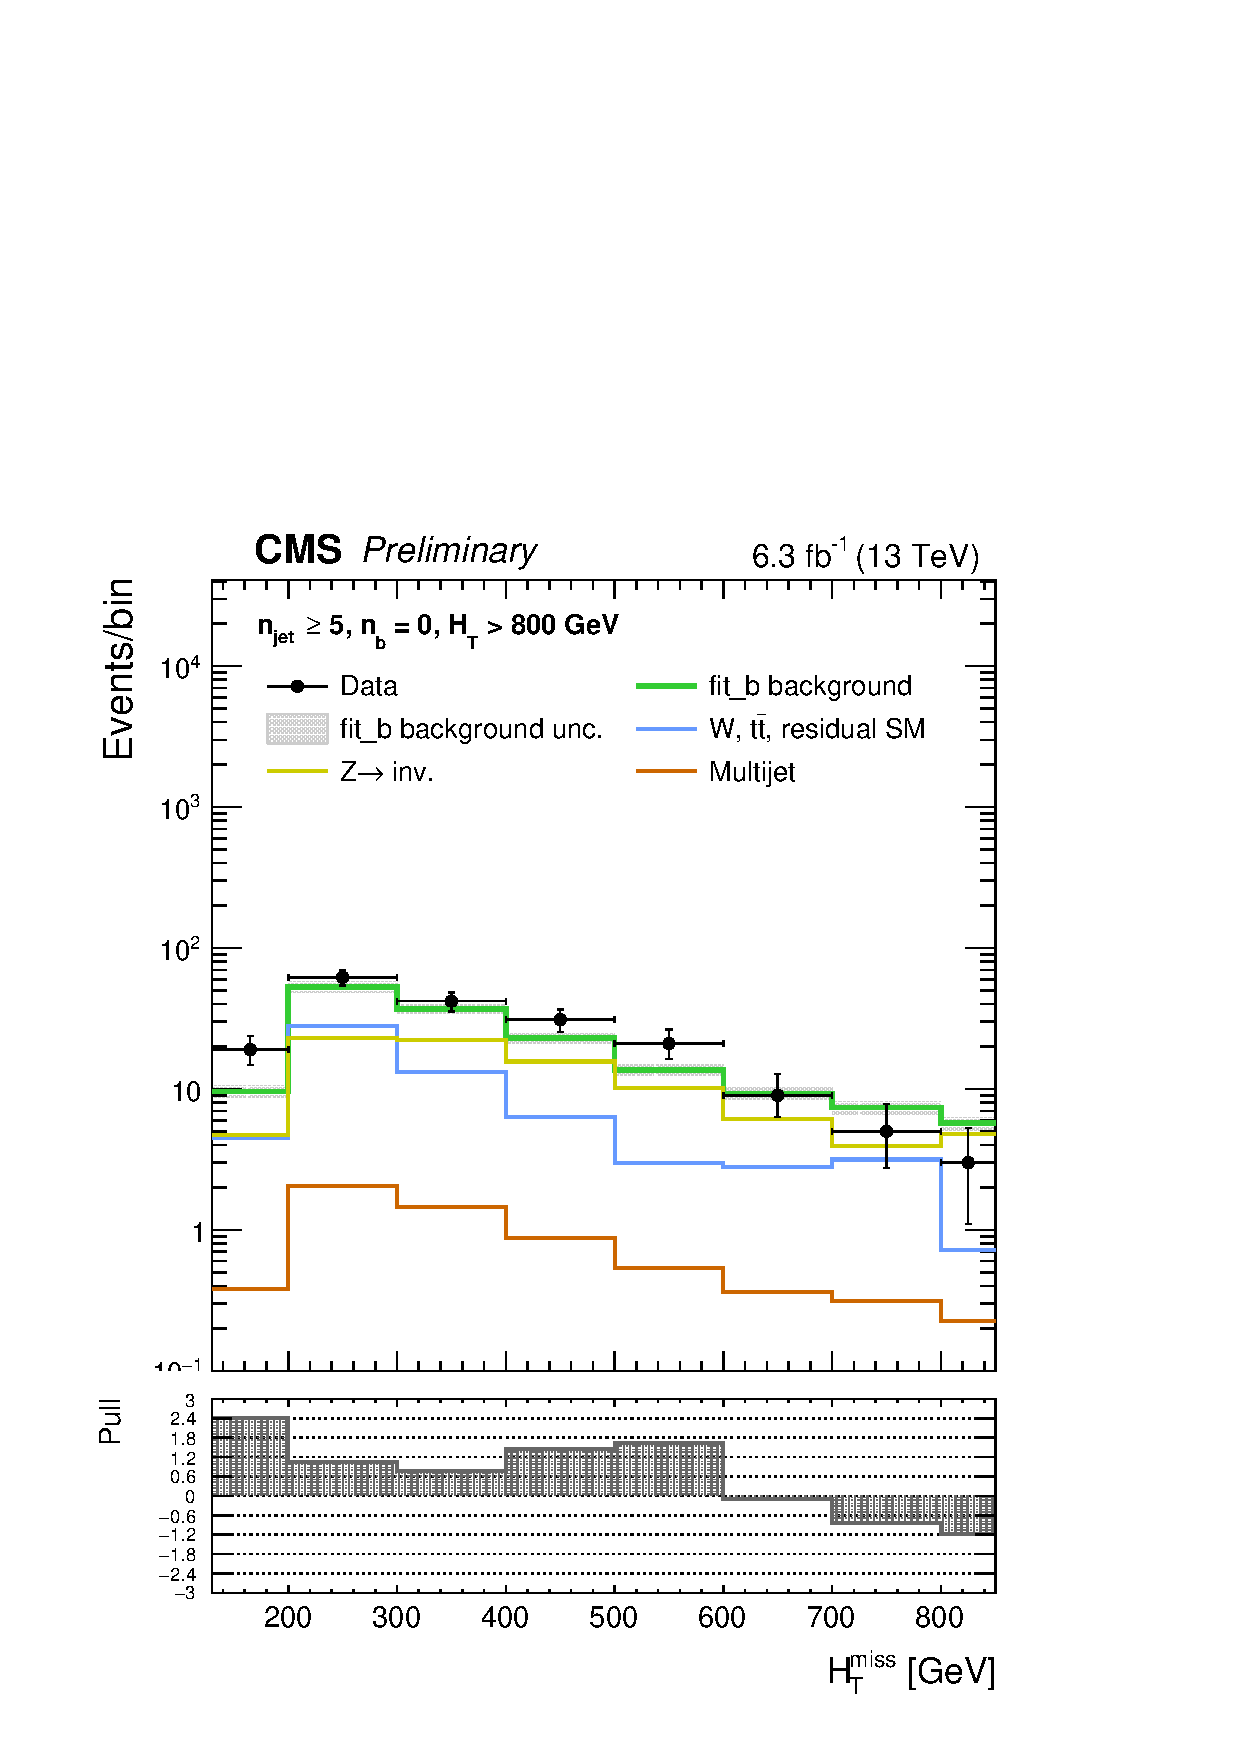
\includegraphics[width=0.45\textwidth]{figures/postFitResults/shapePlots/mhtShape_eq0b_ge5j_800_Inf_fit_b} } ~~
    \subfigure[$\njet = 2$, $\nb = 0$, $300 < \scalht < 350$ GeV]{ 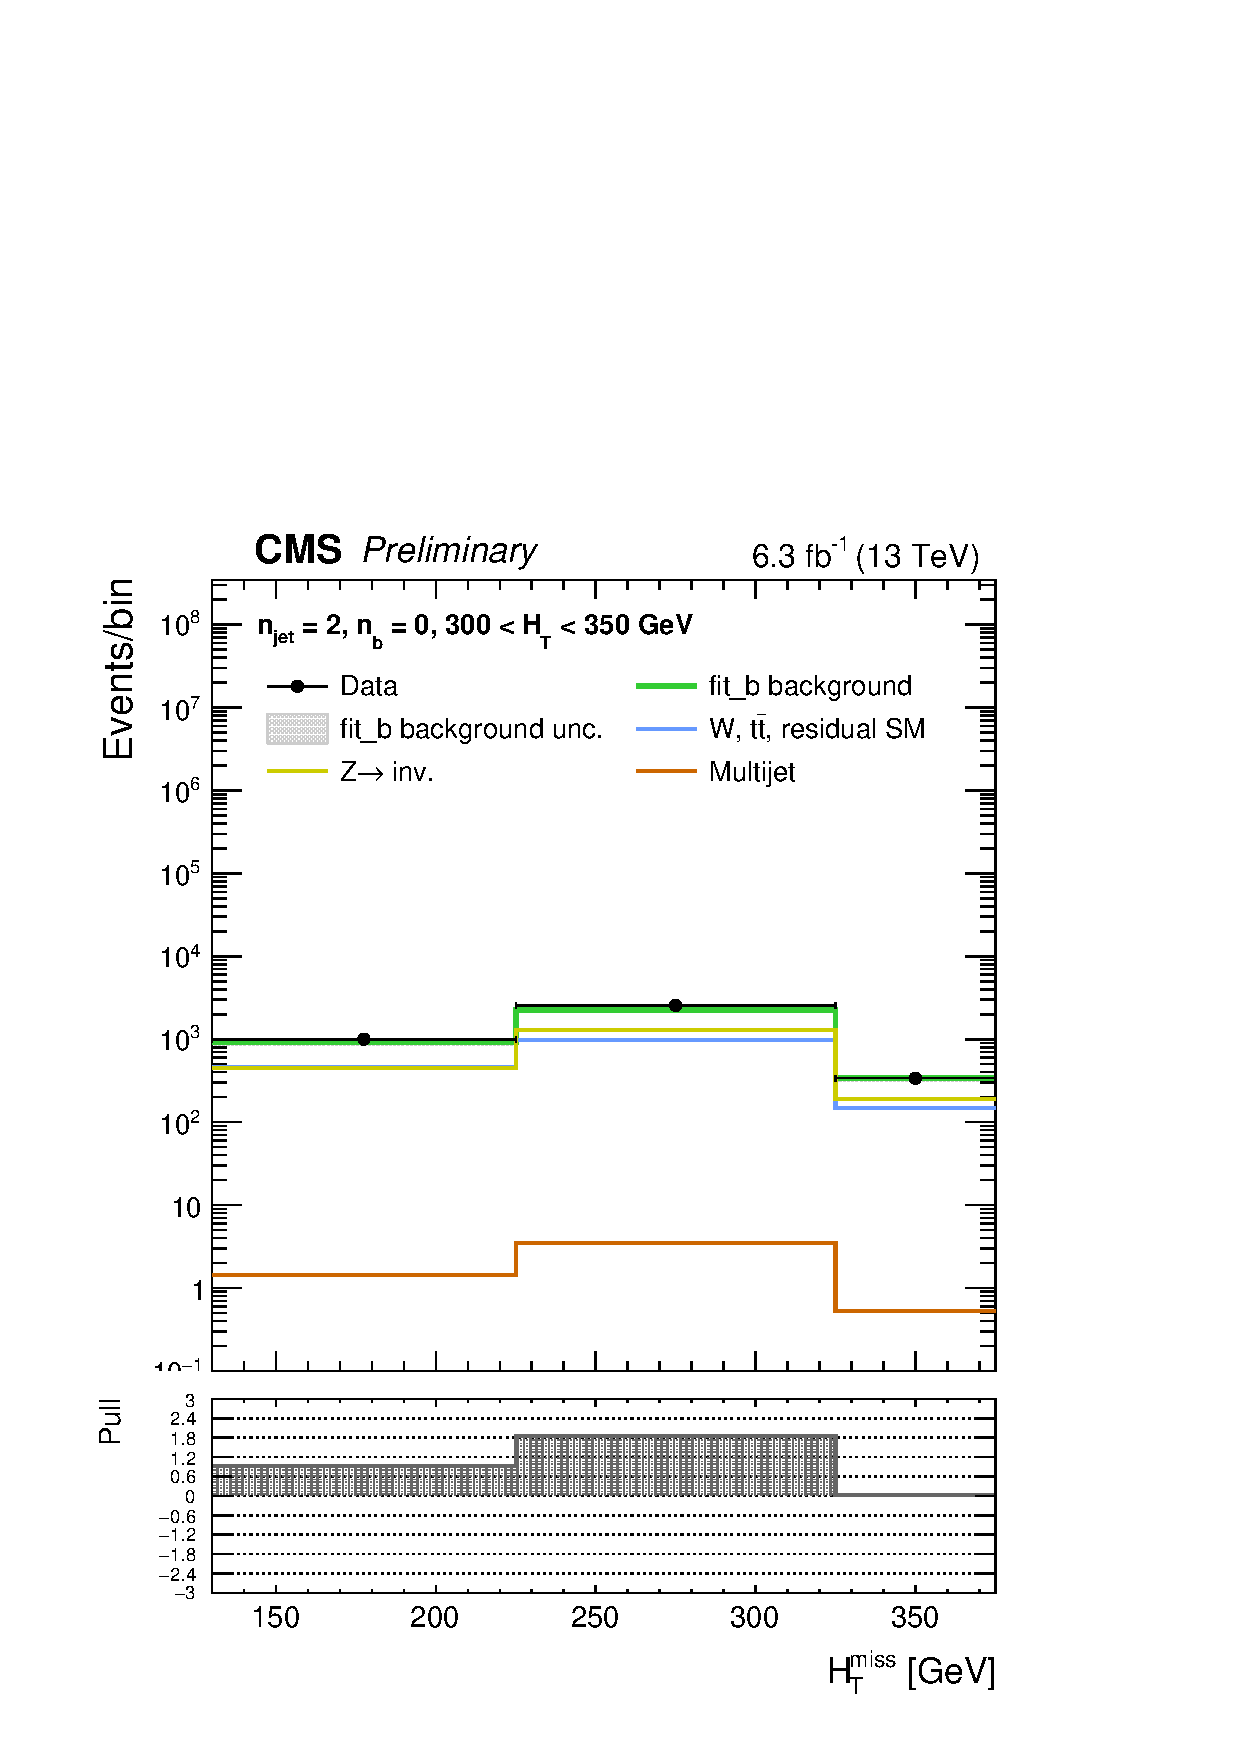
\includegraphics[width=0.45\textwidth]{figures/postFitResults/shapePlots/mhtShape_eq0b_eq2j_300_350_fit_b} } \\
  \end{center}
\end{figure}






\clearpage
\begin{figure}[tbhp]
    \caption{ Pull of the nuisances parameters associated to the \alt-extrapolation systematic uncertainty, 
      for the asymmetric (symmetric) categories on the left (right).
      \label{fig:nuisPull_AlphaT}}
  \begin{center}
    \subfigure[Asymmetric categories]{ 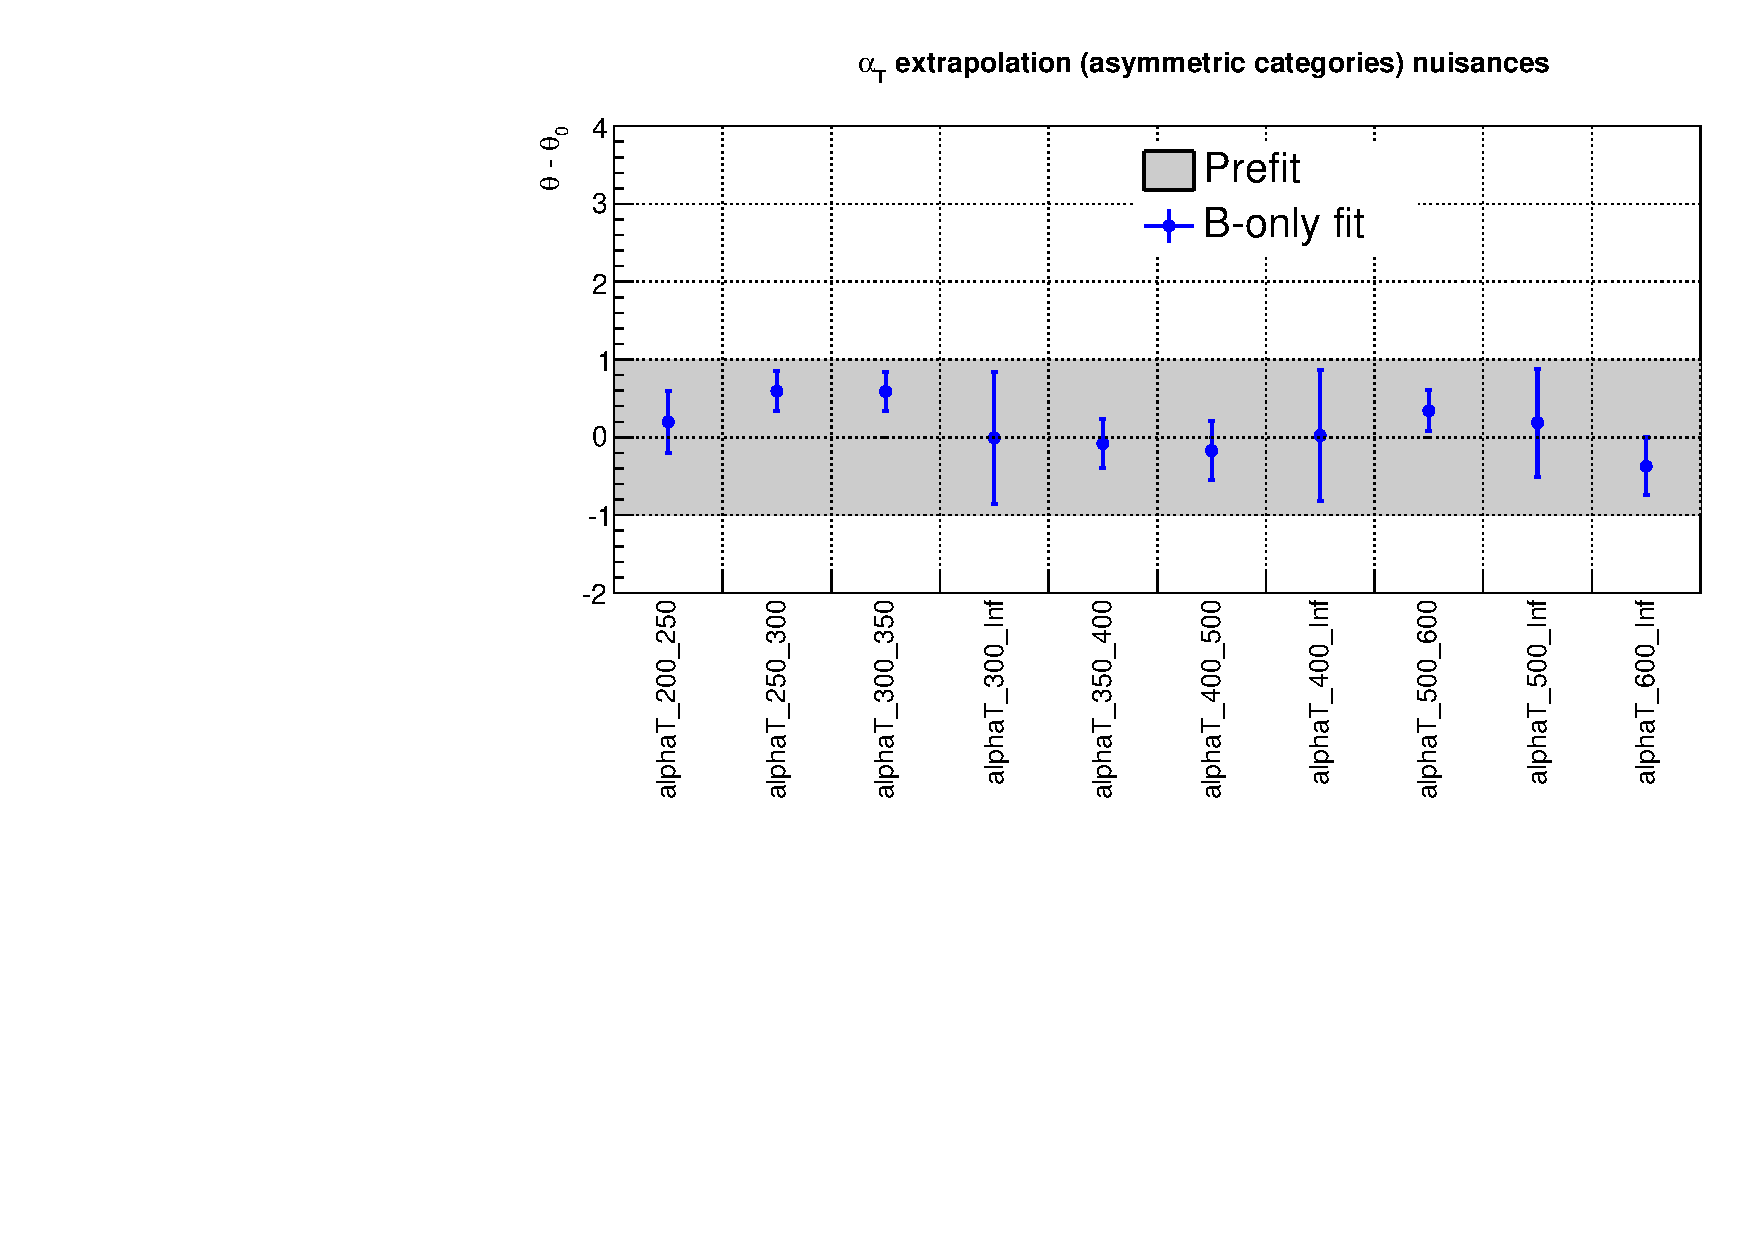
\includegraphics[width=0.45\textwidth]{figures/postFitResults/nuisancePlots/AlphaT_asym_nuisances} } ~~
    \subfigure[Symmetric categories]{ 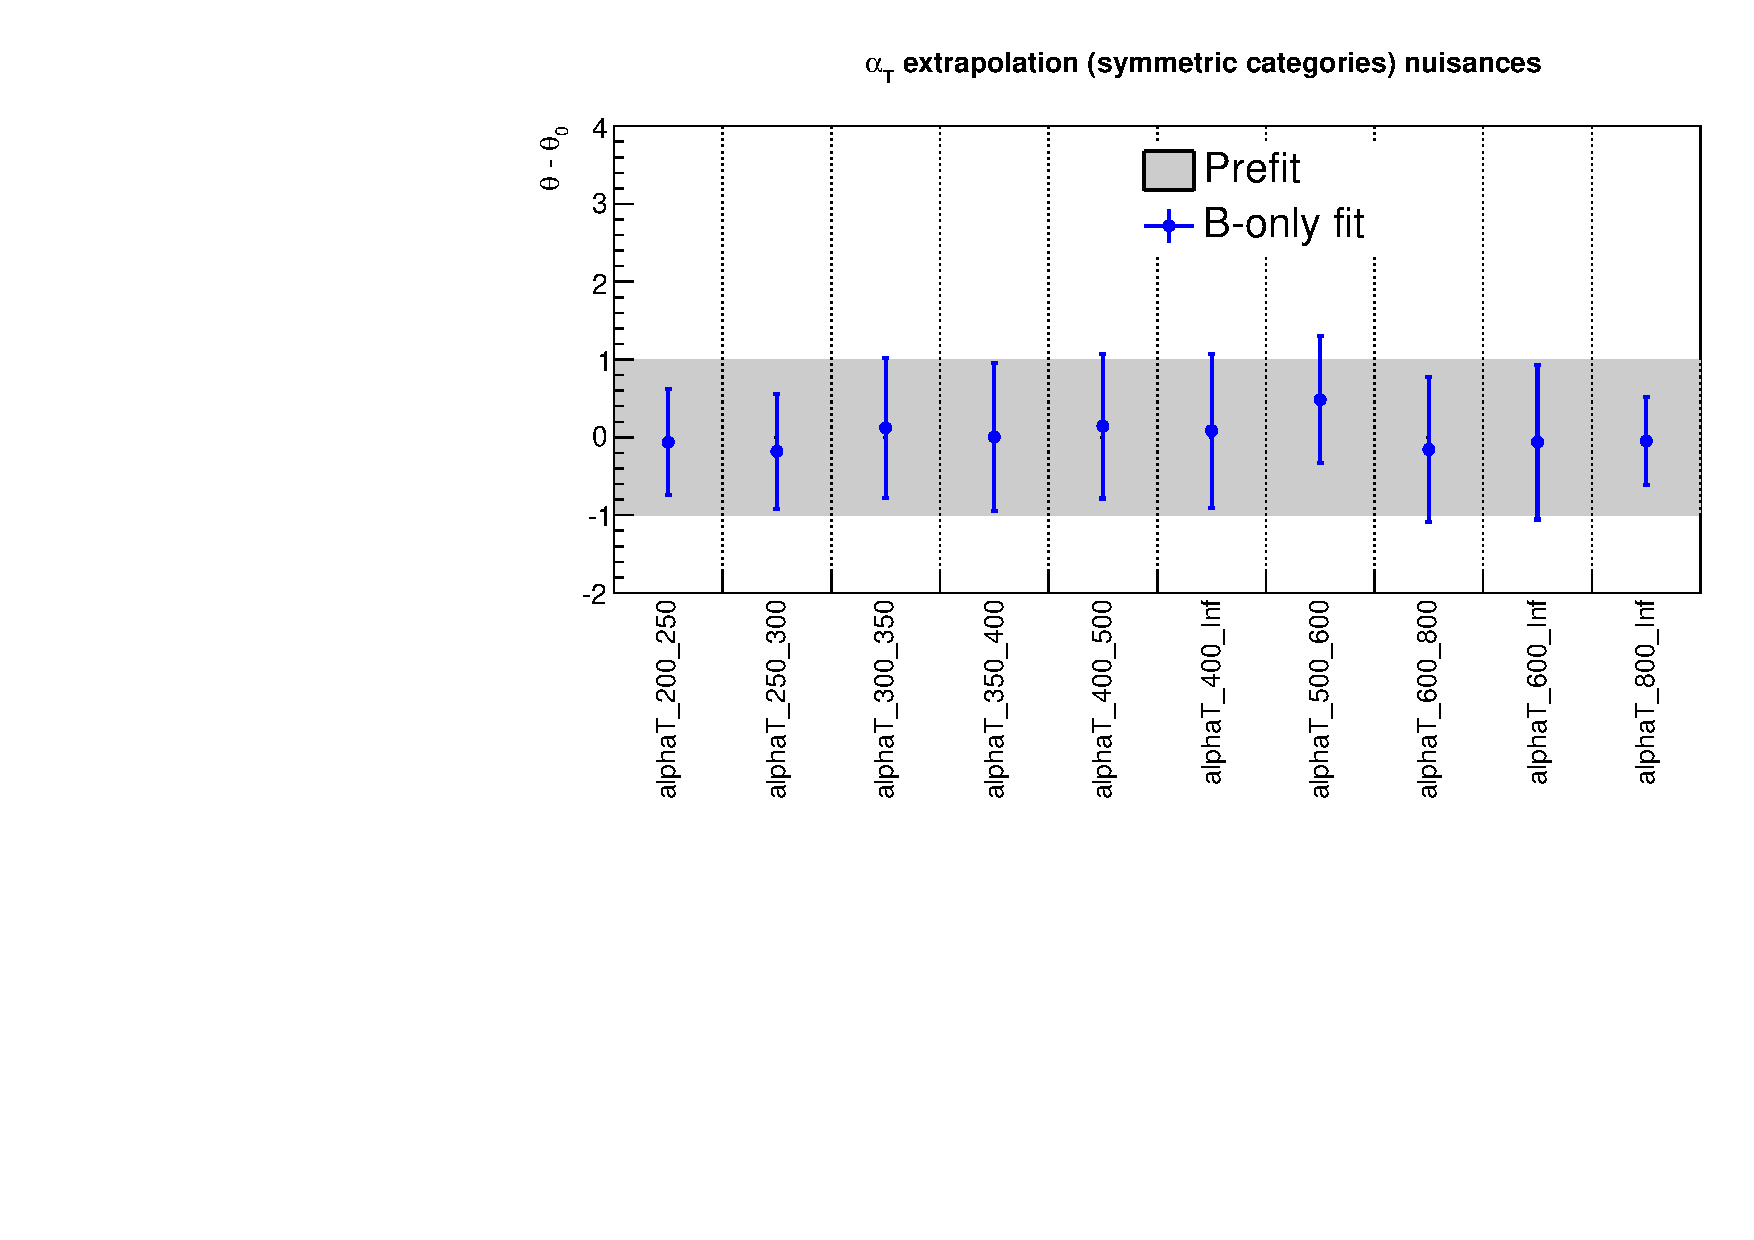
\includegraphics[width=0.45\textwidth]{figures/postFitResults/nuisancePlots/AlphaT_sym_nuisances} }
  \end{center}
\end{figure}

\begin{figure}[tbhp]
    \caption{ Pull of the nuisances parameters associated to the $\gamma/Z$ ratio systematic uncertainty, 
      for the asymmetric (symmetric) categories on the left (right).
      \label{fig:nuisPull_gamma_Z_ratio}}
  \begin{center}
    \subfigure[Asymmetric categories]{ 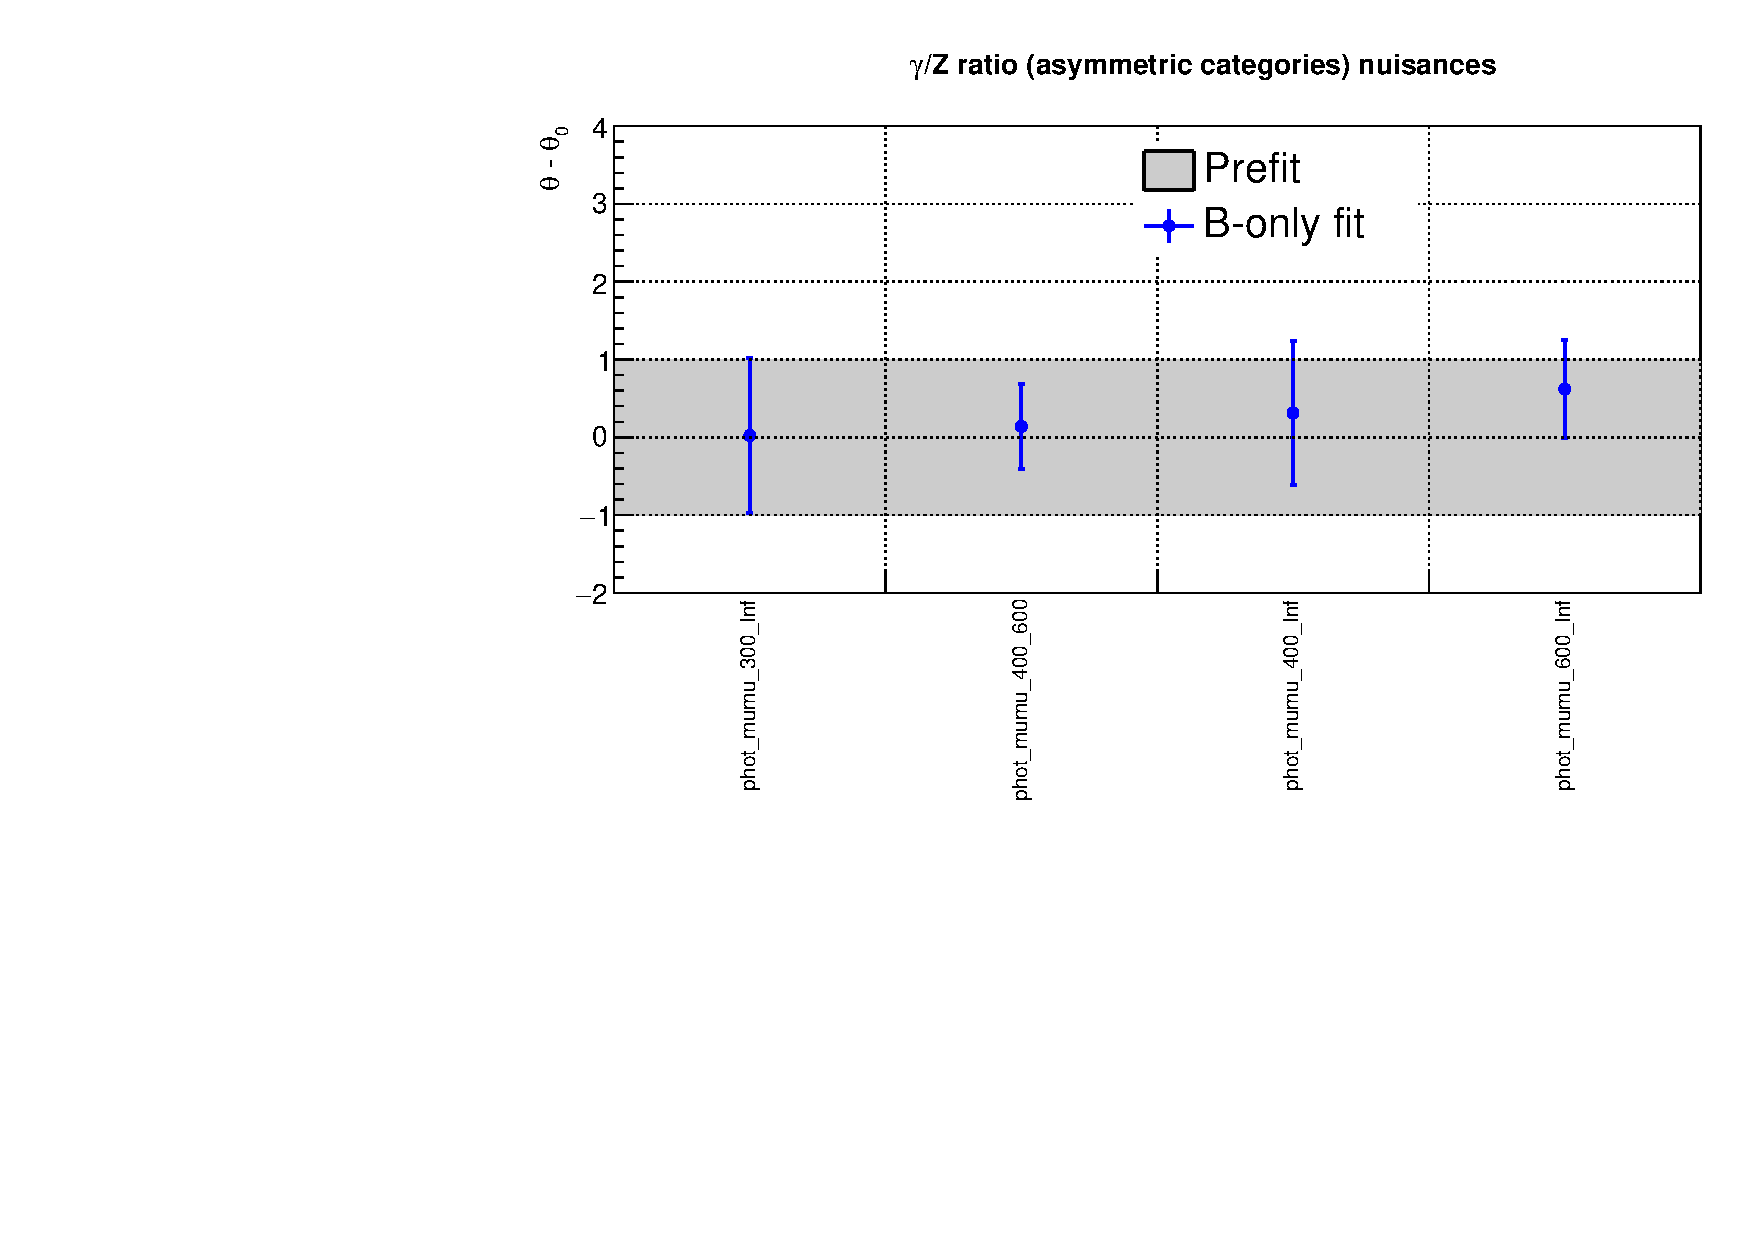
\includegraphics[width=0.45\textwidth]{figures/postFitResults/nuisancePlots/gamma_Z_ratio_asym_nuisances} } ~~
    \subfigure[Symmetric categories]{ 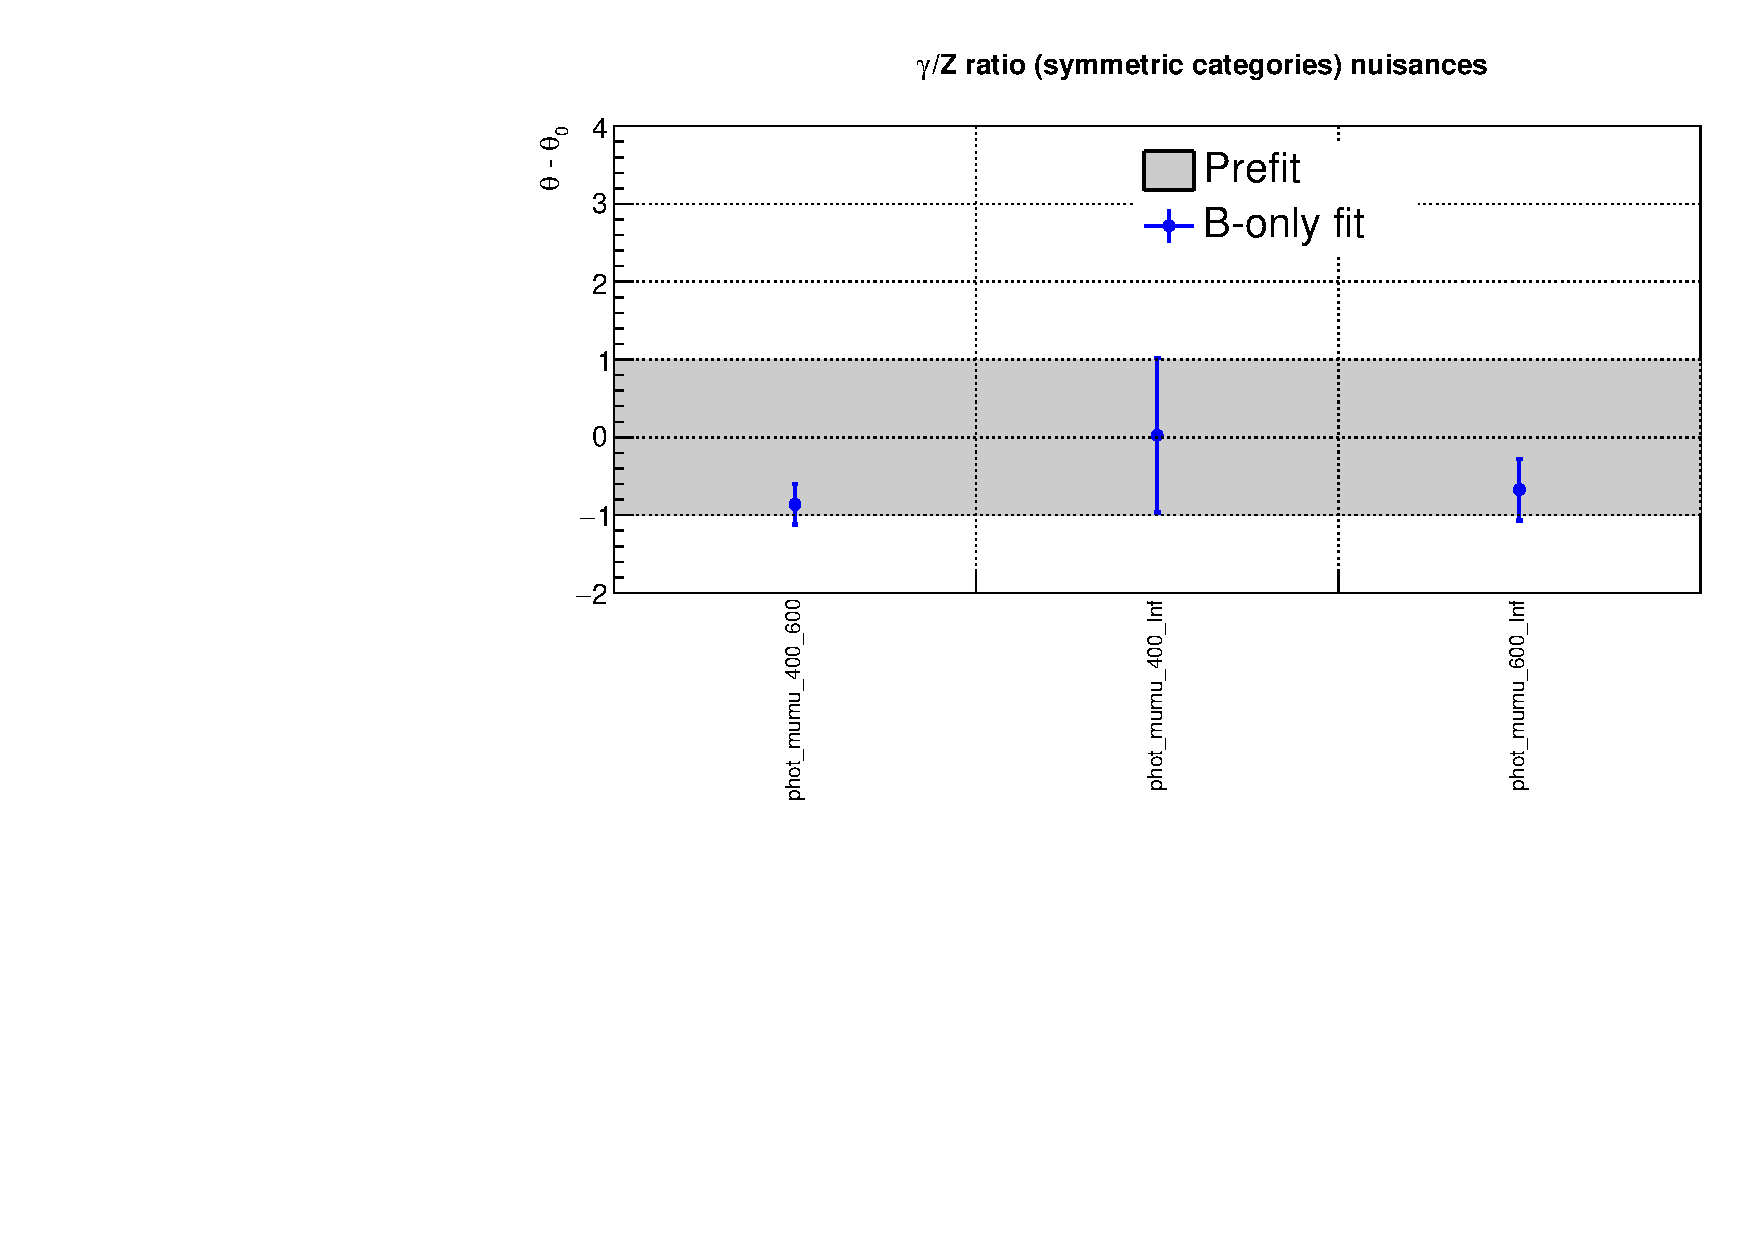
\includegraphics[width=0.45\textwidth]{figures/postFitResults/nuisancePlots/gamma_Z_ratio_sym_nuisances} }
  \end{center}
\end{figure}

\begin{figure}[tbhp]
    \caption{ Pull of the nuisances parameters associated to the $W/Z$ ratio systematic uncertainty, 
      for the asymmetric (symmetric) categories on the left (right).
      \label{fig:nuisPull_W_Z_ratio}}
  \begin{center}
    \subfigure[Asymmetric categories]{ 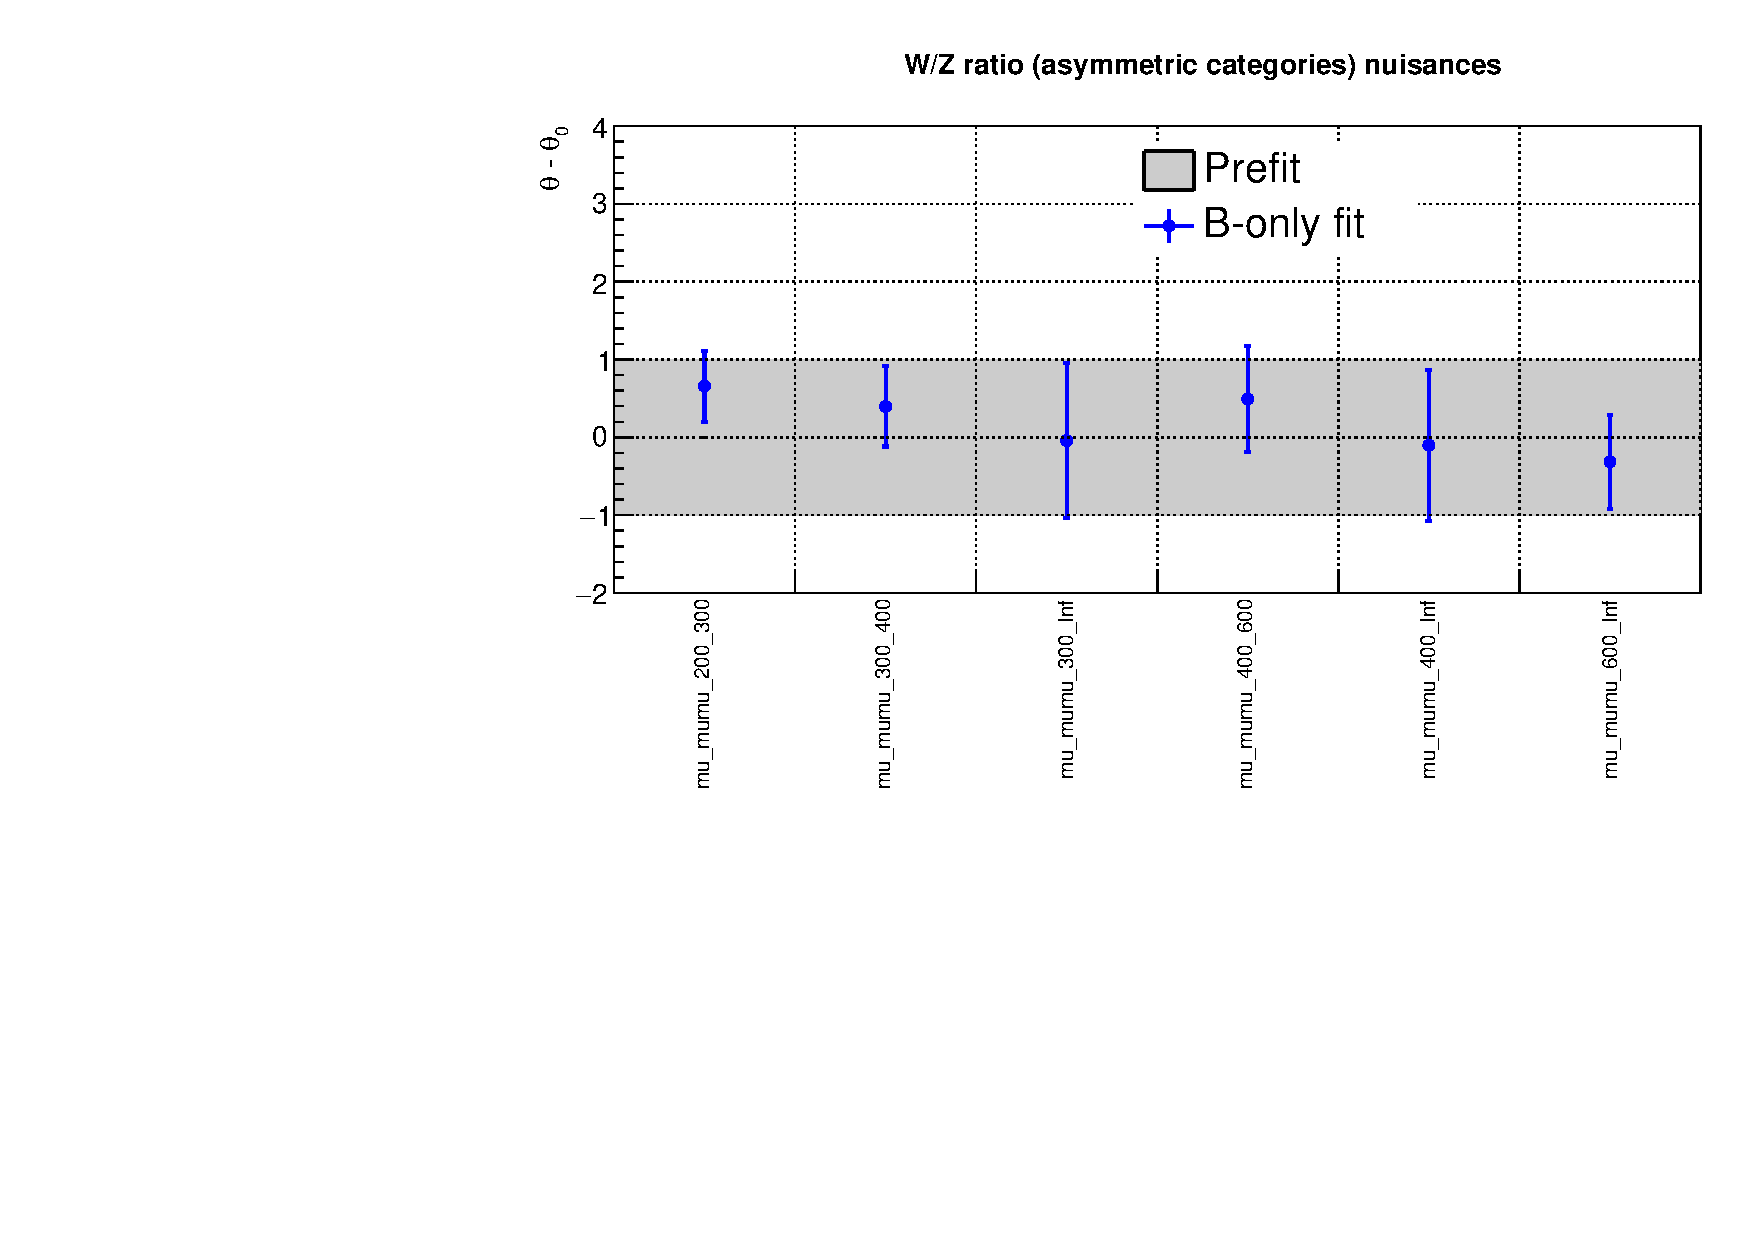
\includegraphics[width=0.45\textwidth]{figures/postFitResults/nuisancePlots/W_Z_ratio_asym_nuisances} } ~~
    \subfigure[Symmetric categories]{ 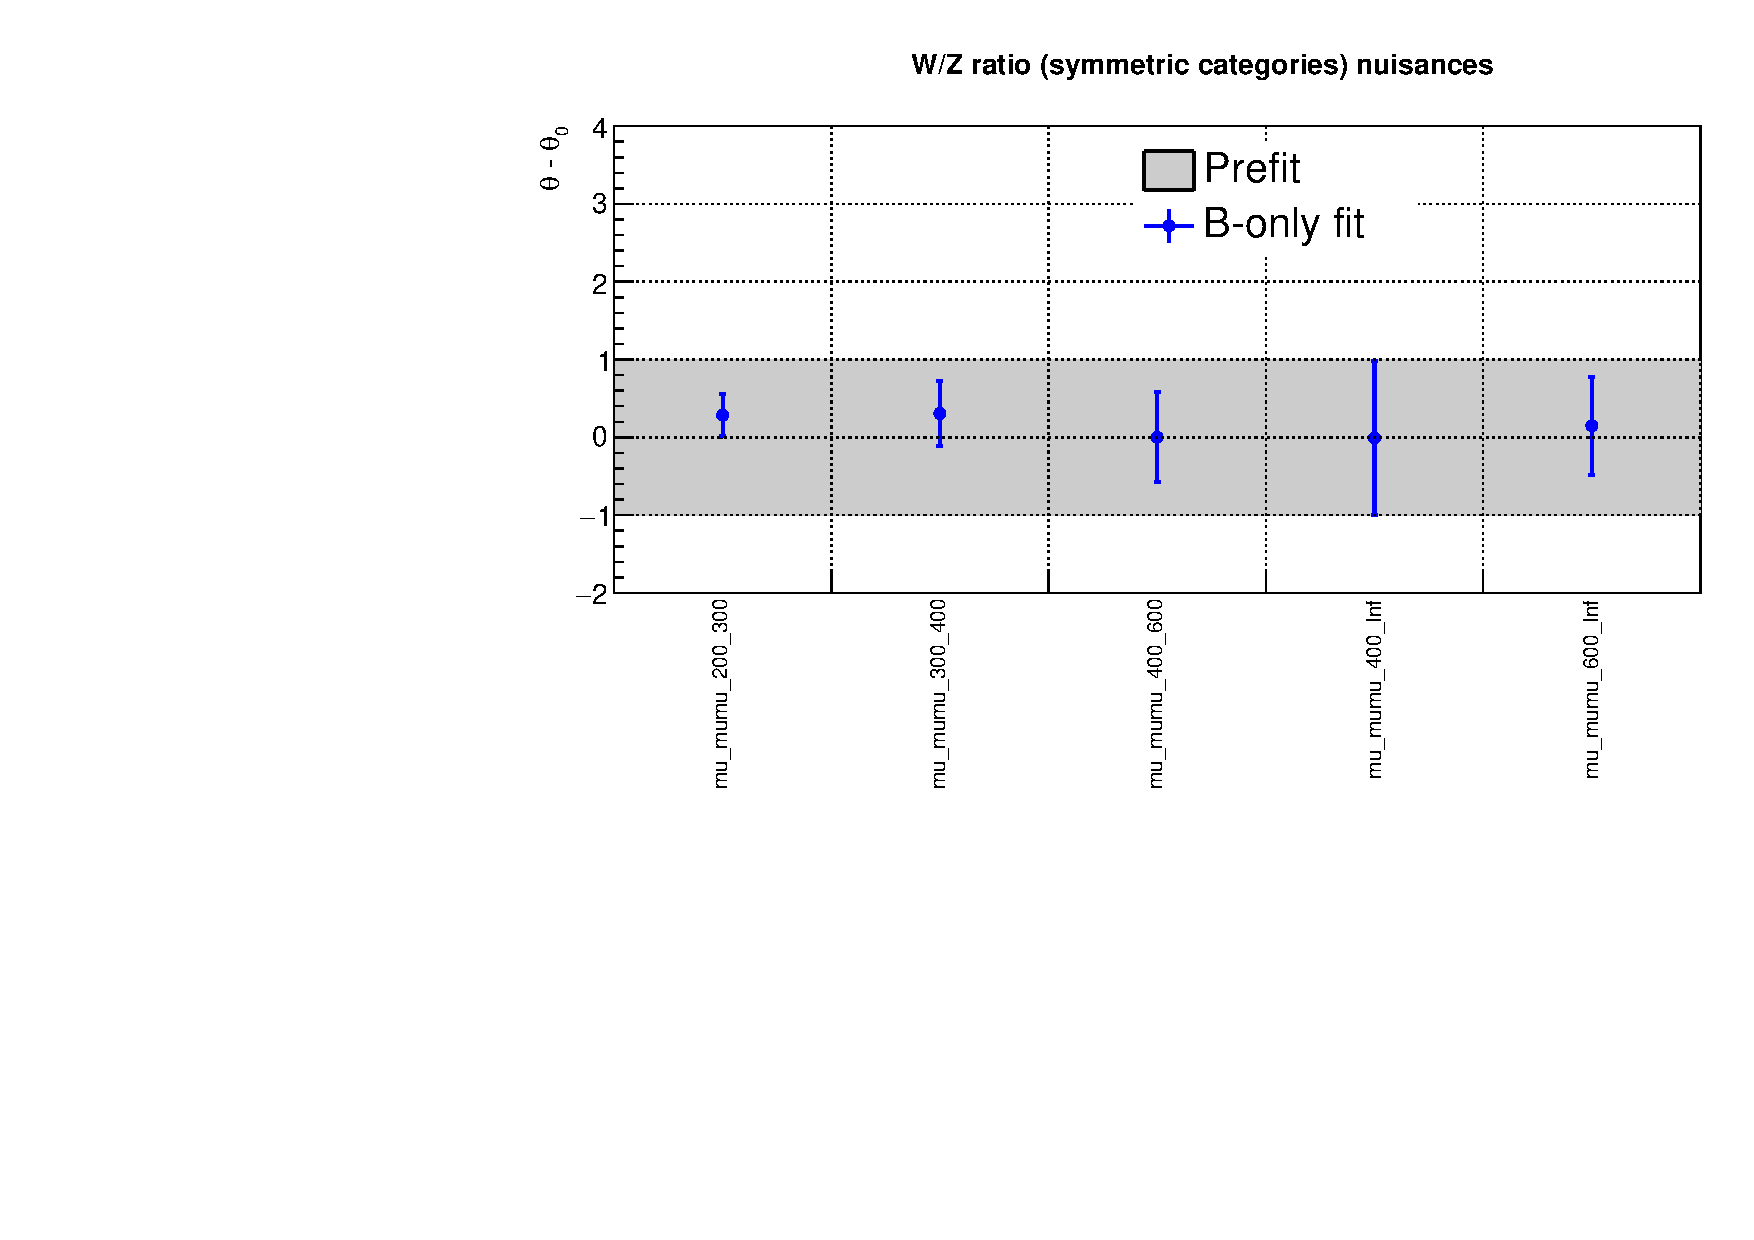
\includegraphics[width=0.45\textwidth]{figures/postFitResults/nuisancePlots/W_Z_ratio_sym_nuisances} }
  \end{center}
\end{figure}


\begin{figure}[tbhp]
    \caption{ Pull of the nuisances parameters associated to the $\ttbar/W$ admixture systematic uncertainty, 
      for the asymmetric (symmetric) categories on the left (right).
      \label{fig:nuisPull_tt_W_admixture}}
  \begin{center}
    \subfigure[Asymmetric categories]{ 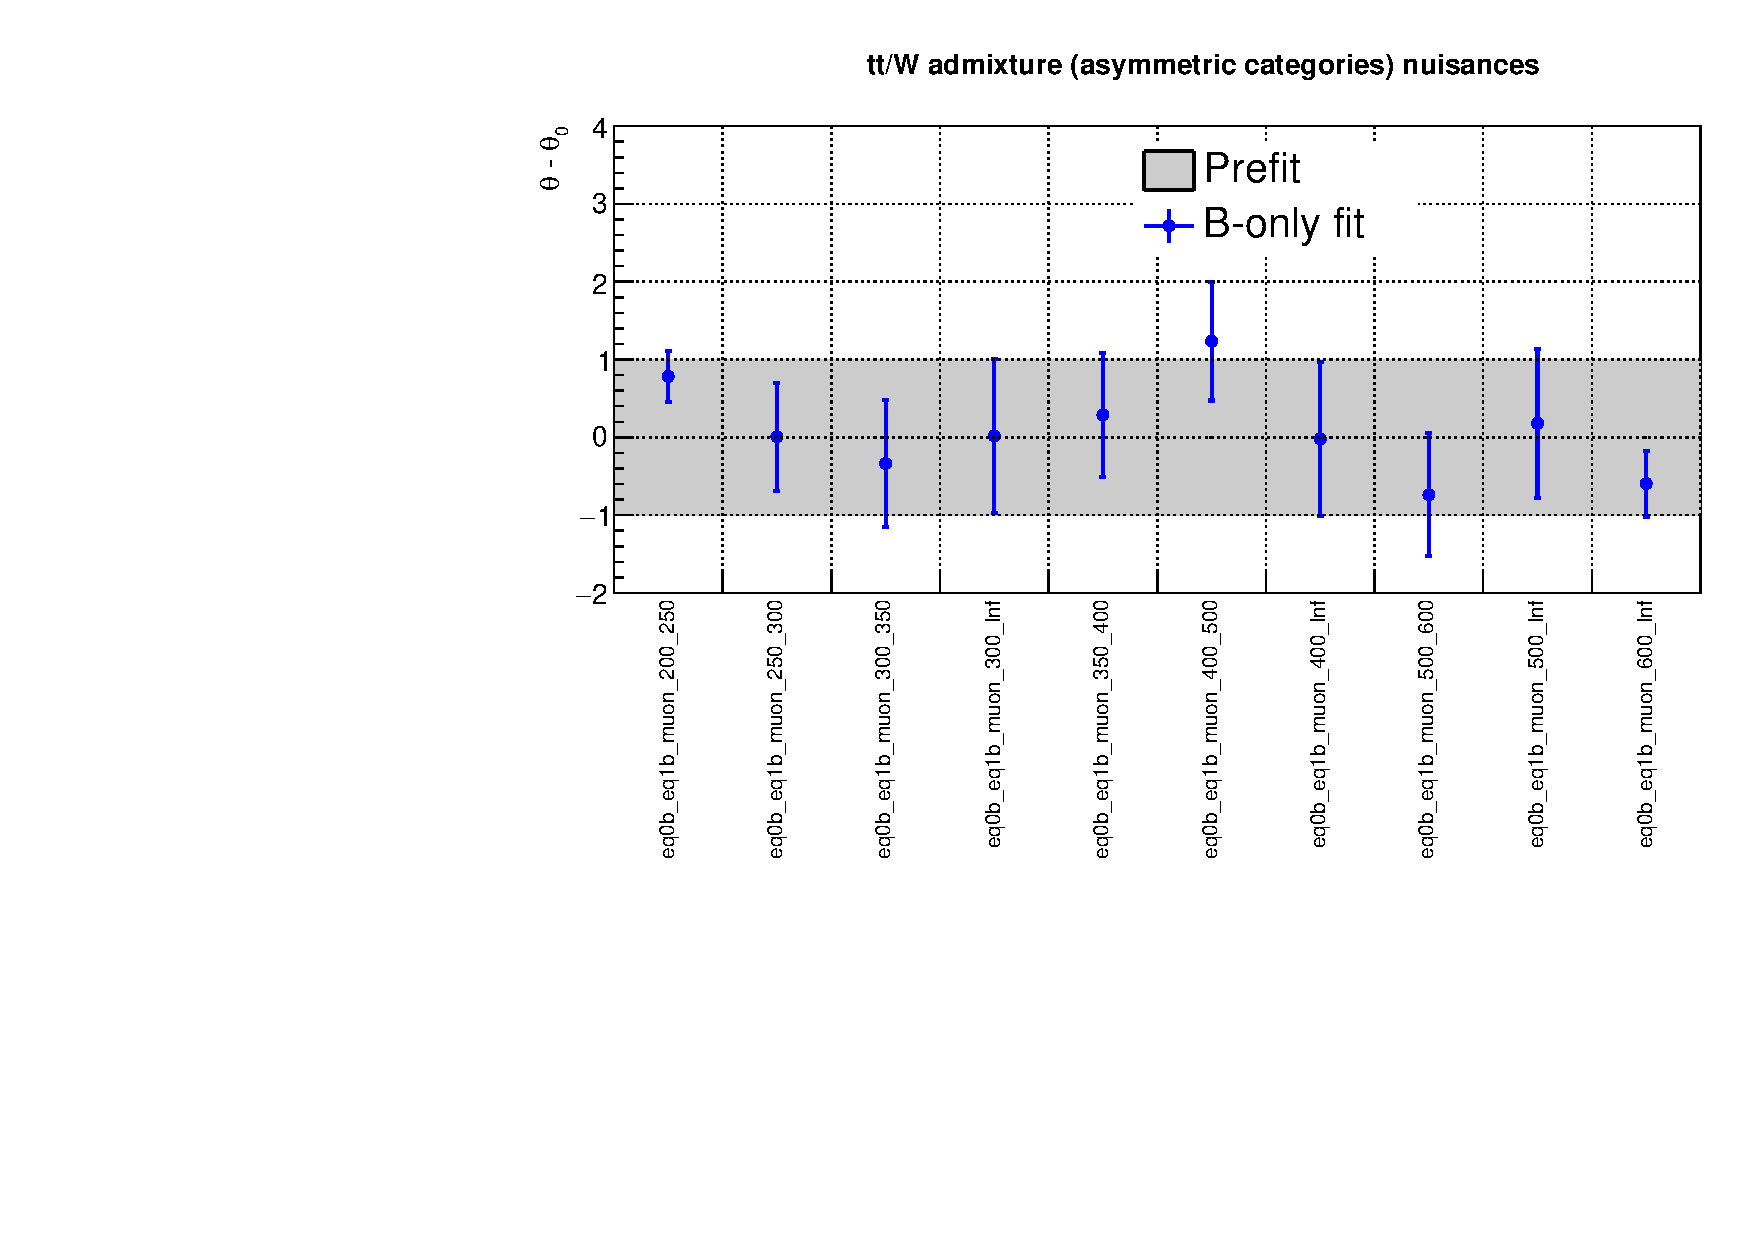
\includegraphics[width=0.45\textwidth]{figures/postFitResults/nuisancePlots/tt_W_admixture_asym_nuisances} } ~~
    \subfigure[Symmetric categories]{ 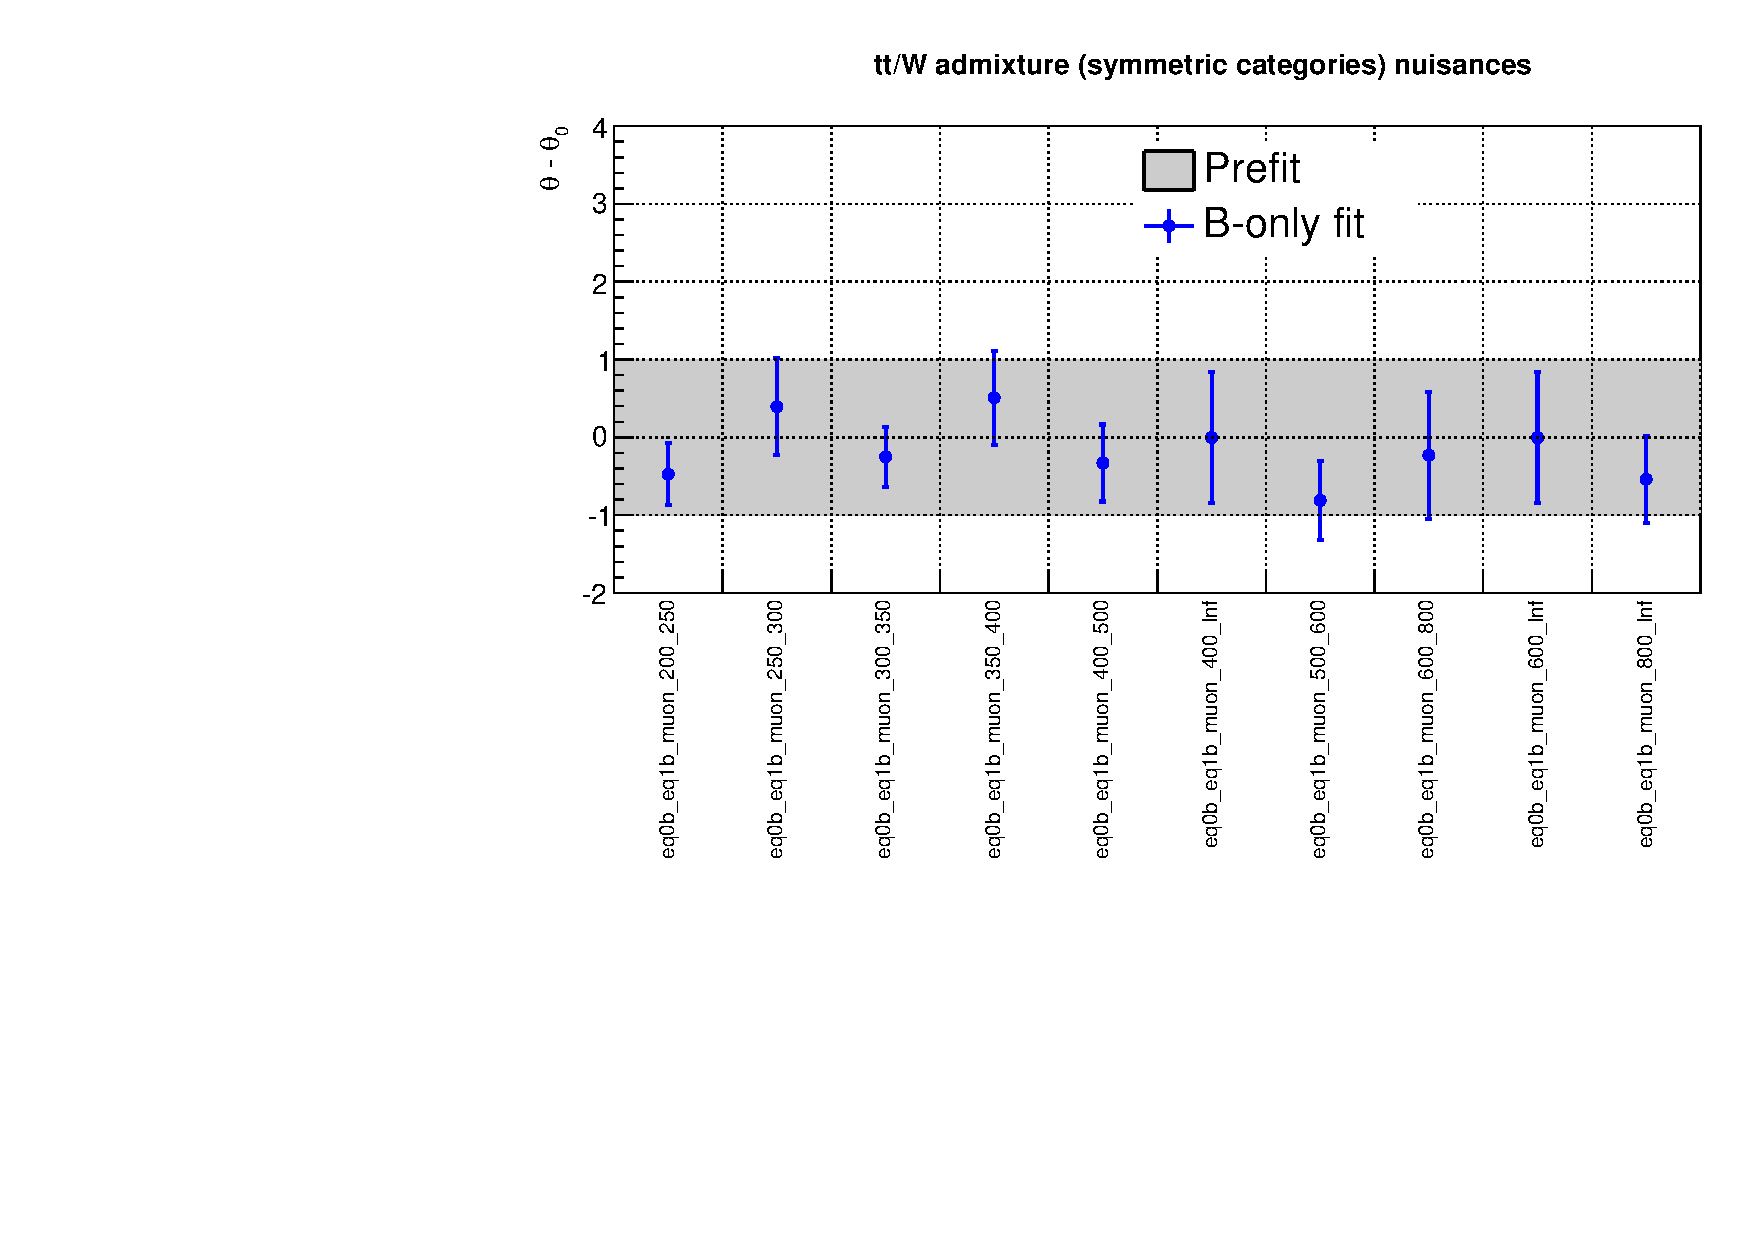
\includegraphics[width=0.45\textwidth]{figures/postFitResults/nuisancePlots/tt_W_admixture_sym_nuisances} }
  \end{center}
\end{figure}


\begin{figure}[tbhp]
    \caption{ Pull of the nuisances parameters associated to the W polarisation systematic uncertainty, 
      for the asymmetric (symmetric) categories on the left (right).
      \label{fig:nuisPull_WPol}}
  \begin{center}
    \subfigure[Asymmetric categories]{ 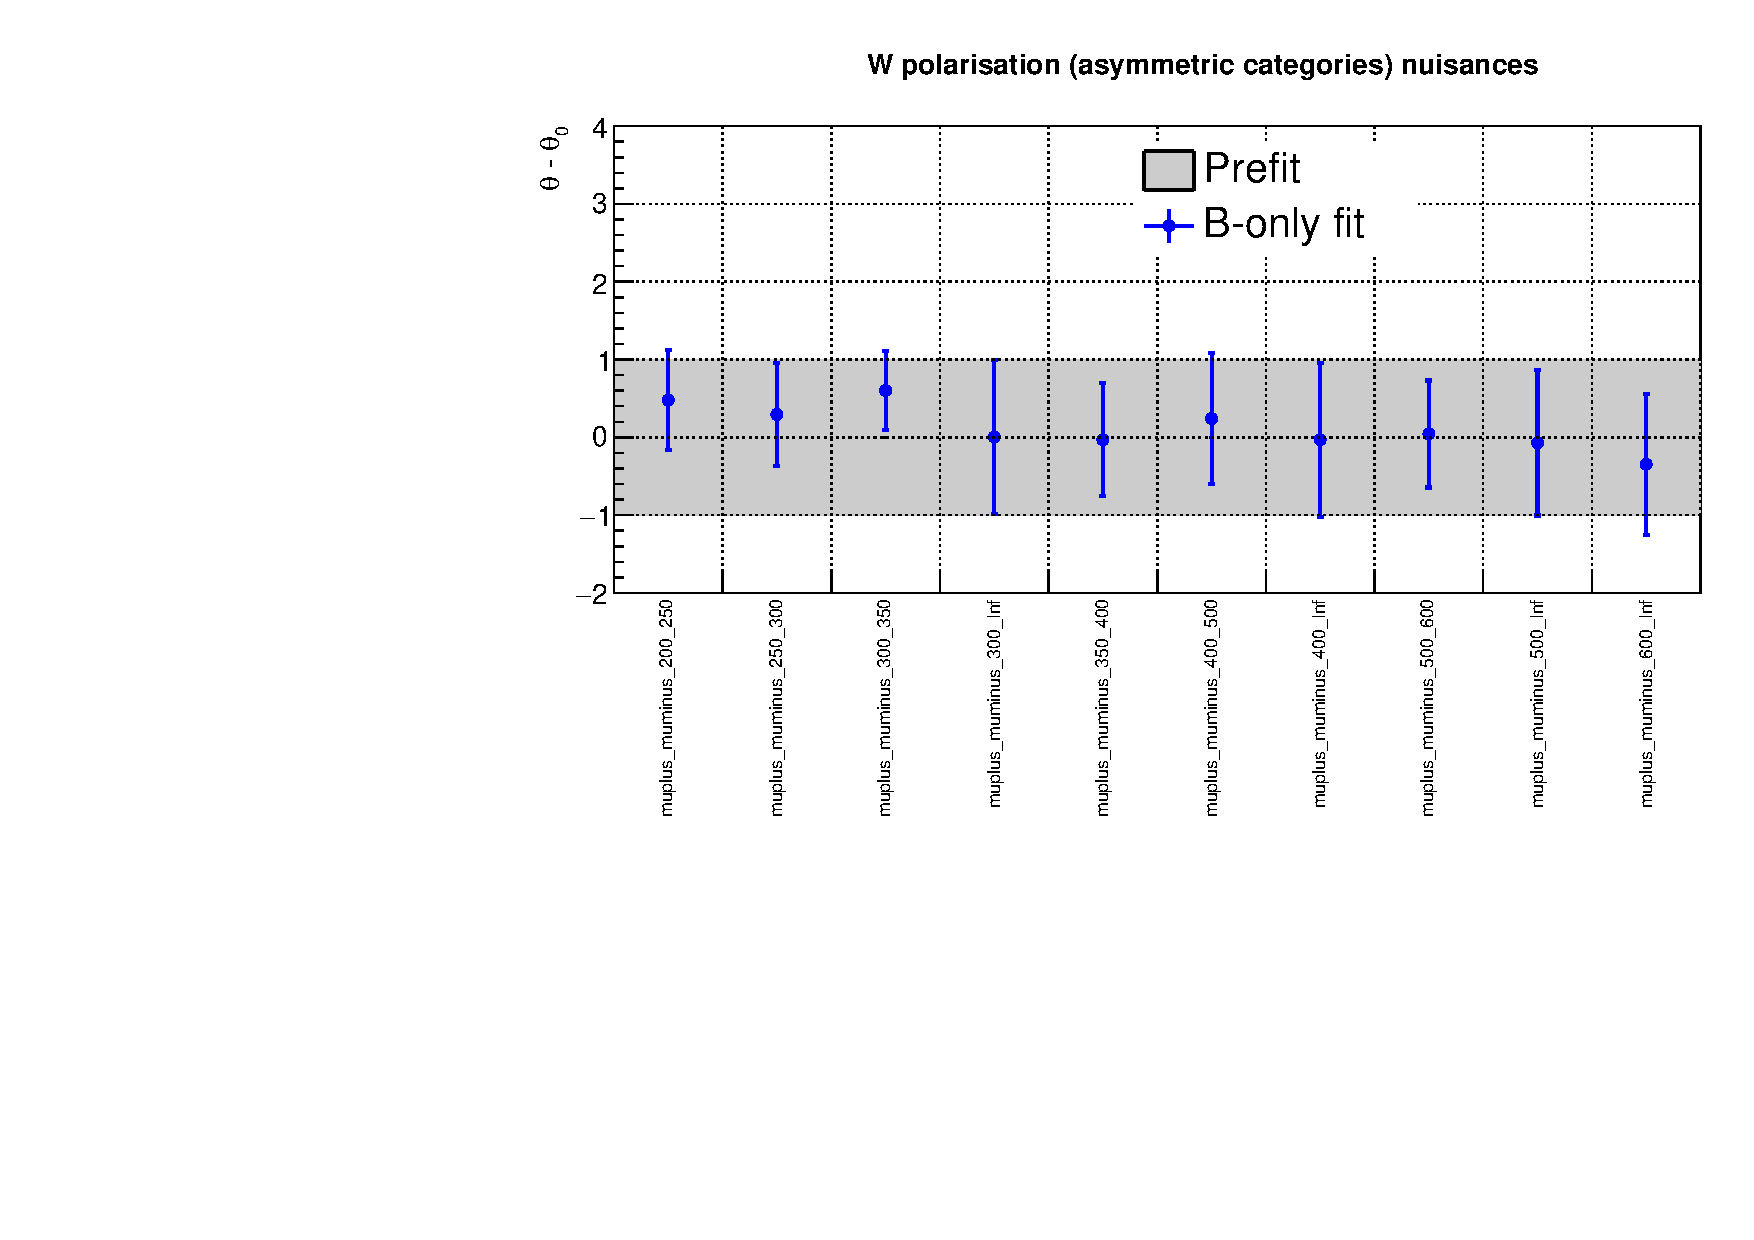
\includegraphics[width=0.45\textwidth]{figures/postFitResults/nuisancePlots/WPol_asym_nuisances} } ~~
    \subfigure[Symmetric categories]{ 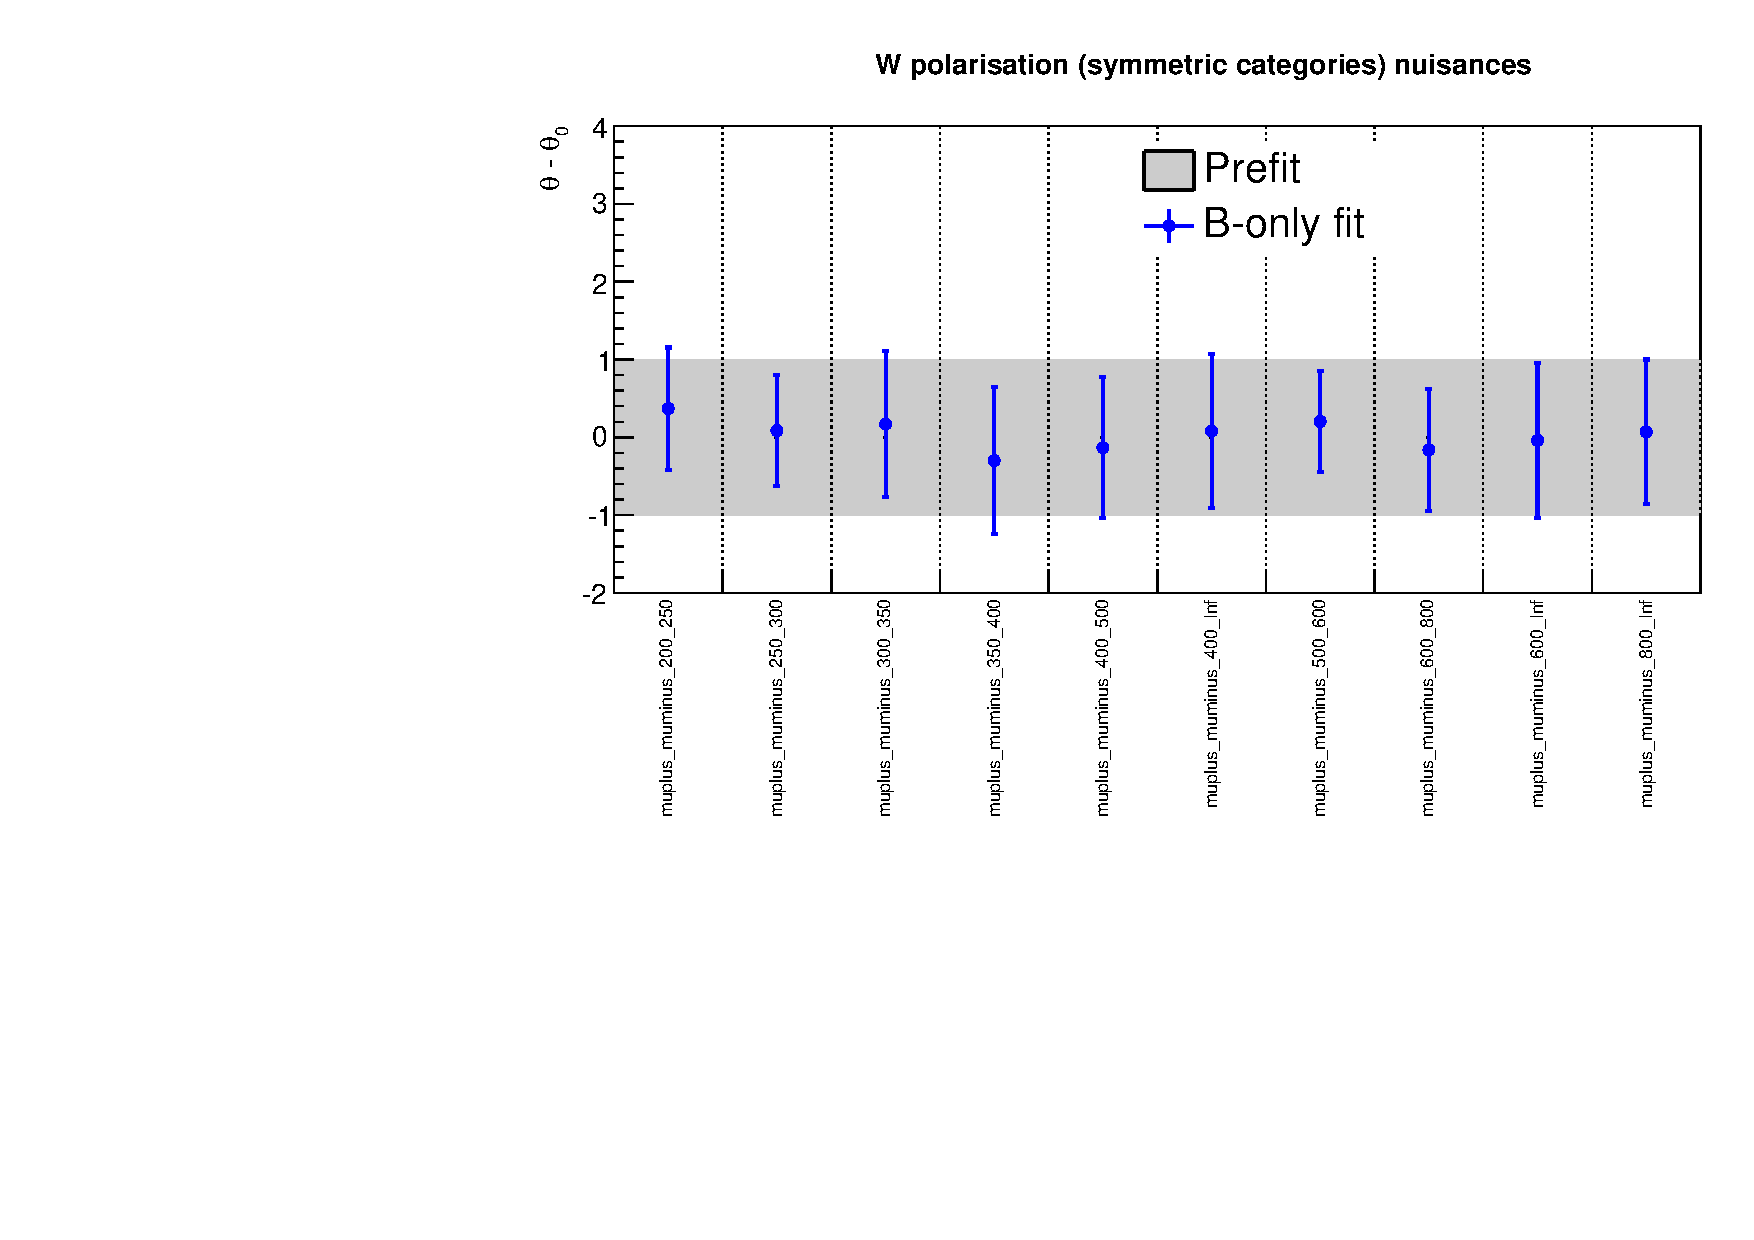
\includegraphics[width=0.45\textwidth]{figures/postFitResults/nuisancePlots/WPol_sym_nuisances} }
  \end{center}
\end{figure}


\begin{figure}[tbhp]
    \caption{ Pull of the nuisances parameters associated to the $\ttbar+W$ template systematic uncertainty, 
      for the asymmetric (symmetric) categories on the left (right).
      \label{fig:nuisPull_TemplateTtw}}
  \begin{center}
    \subfigure[Asymmetric categories]{ 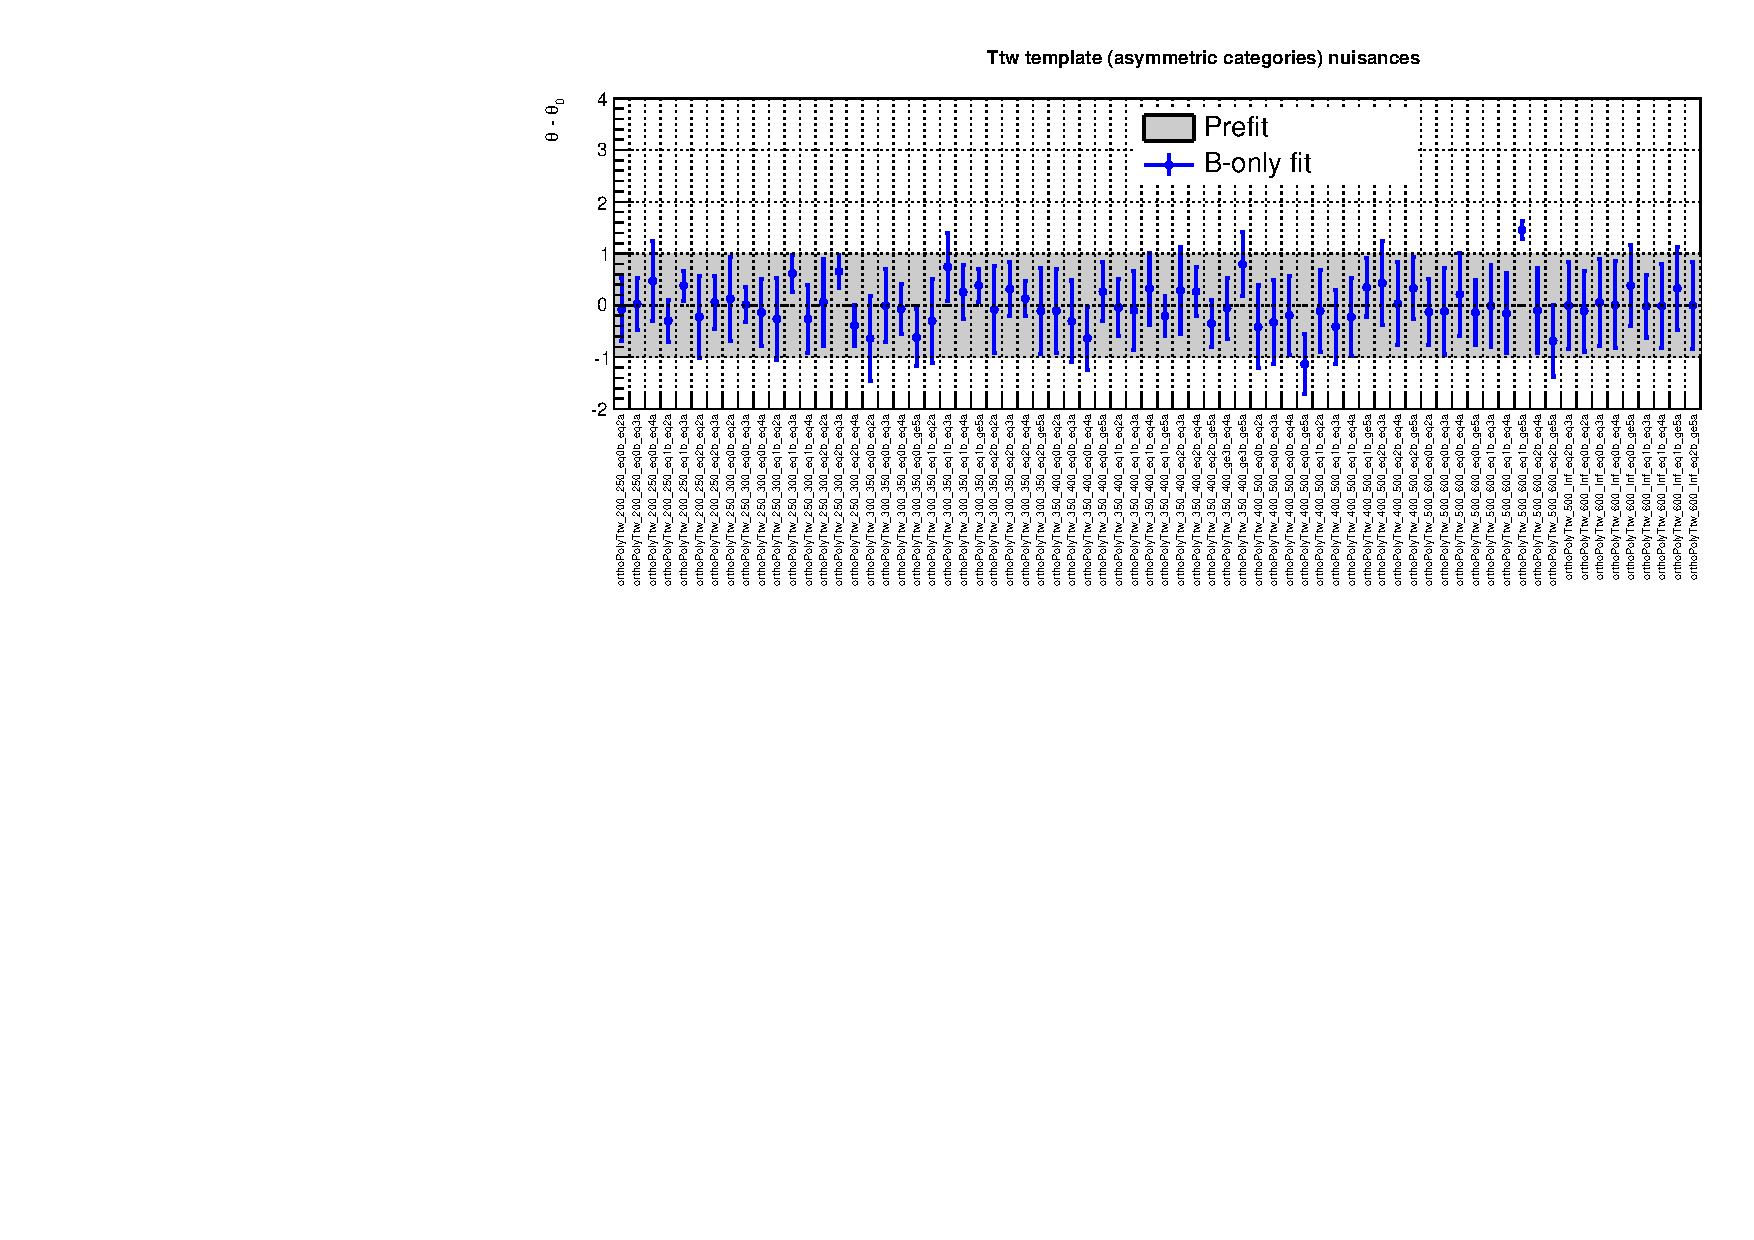
\includegraphics[width=0.8\textwidth]{figures/postFitResults/nuisancePlots/TemplateTtw_asym_nuisances} } \\
    \subfigure[Symmetric categories]{ 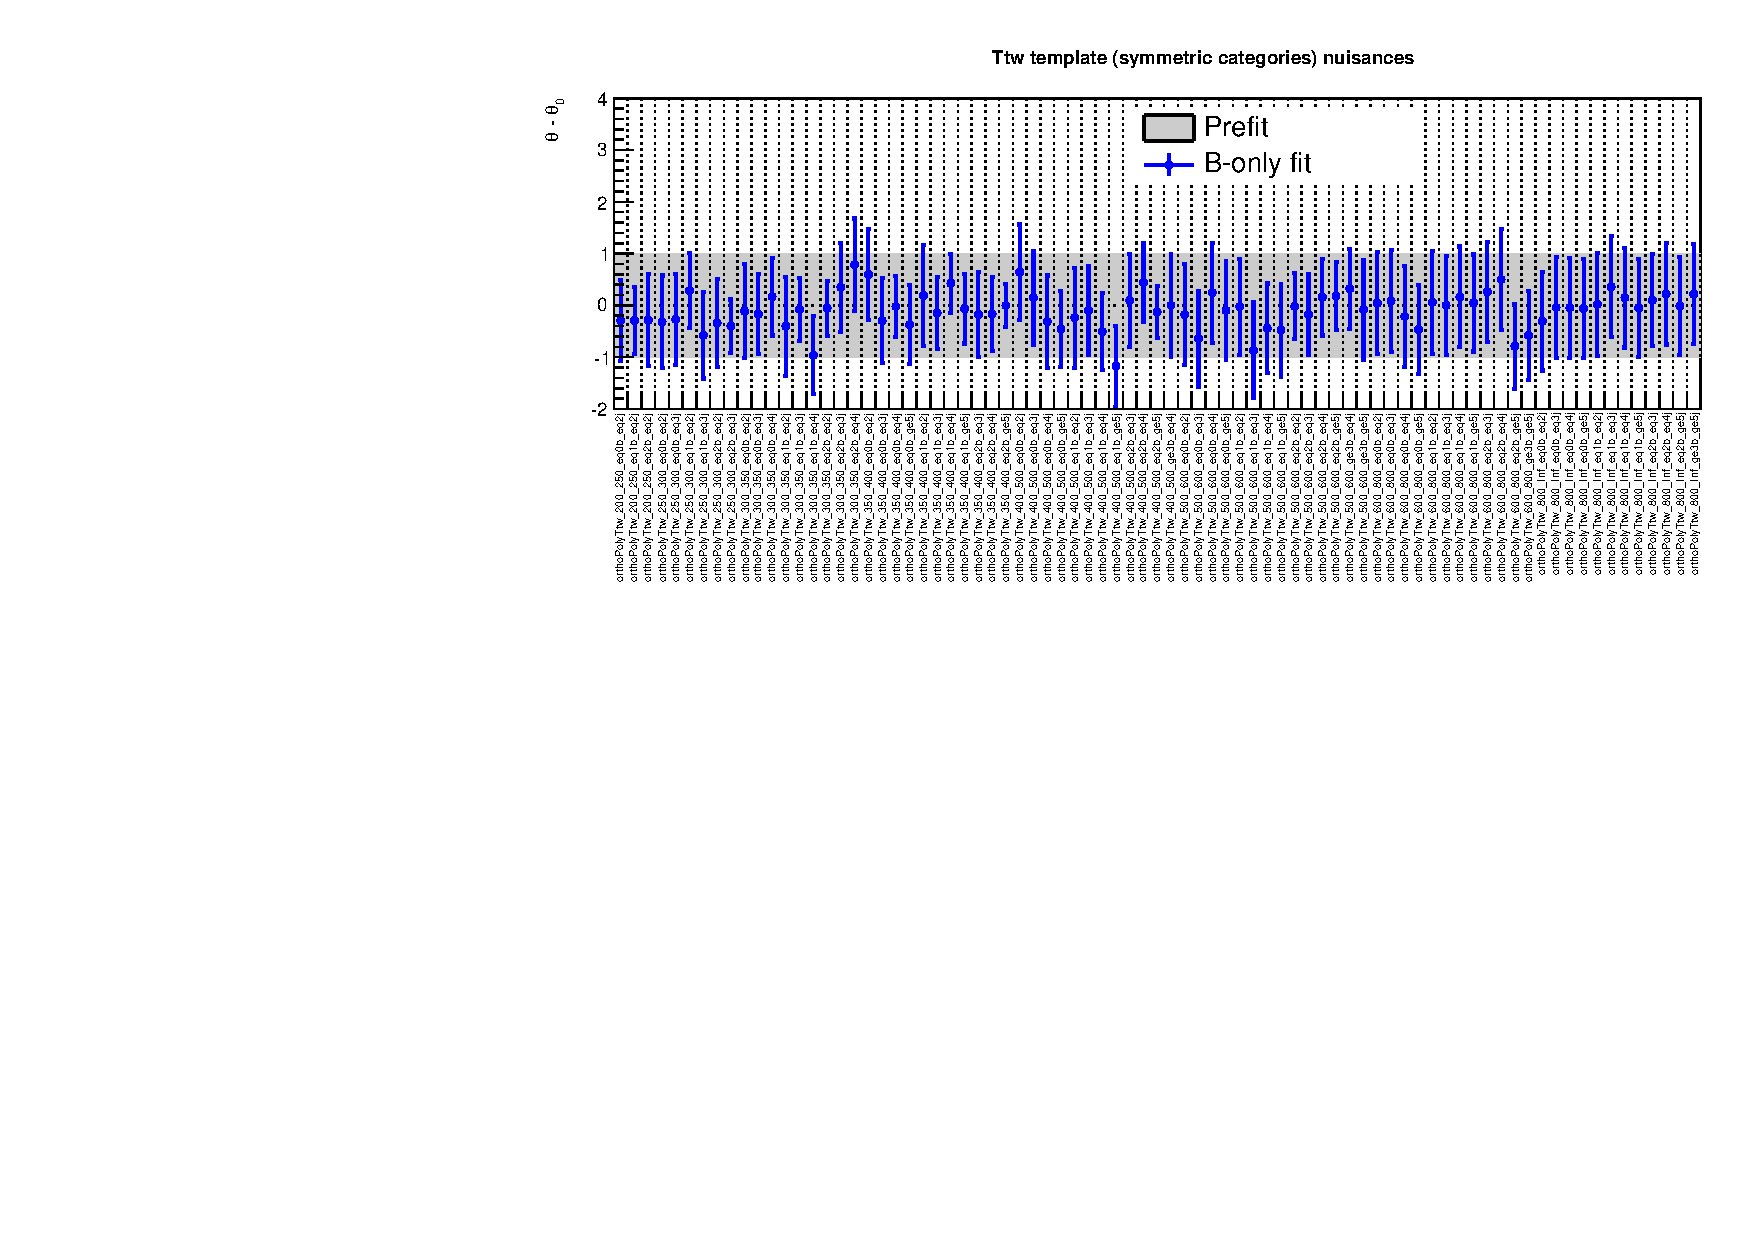
\includegraphics[width=0.8\textwidth]{figures/postFitResults/nuisancePlots/TemplateTtw_sym_nuisances} }
  \end{center}
\end{figure}


\begin{figure}[tbhp]
    \caption{Pull of the nuisances parameters associated to the $Z\rightarrow\nu\nu$ template systematic uncertainty, 
      for the asymmetric (symmetric) categories on the left (right).
      \label{fig:nuisPull_TemplateZinv}}
  \begin{center}
    \subfigure[Asymmetric categories]{ 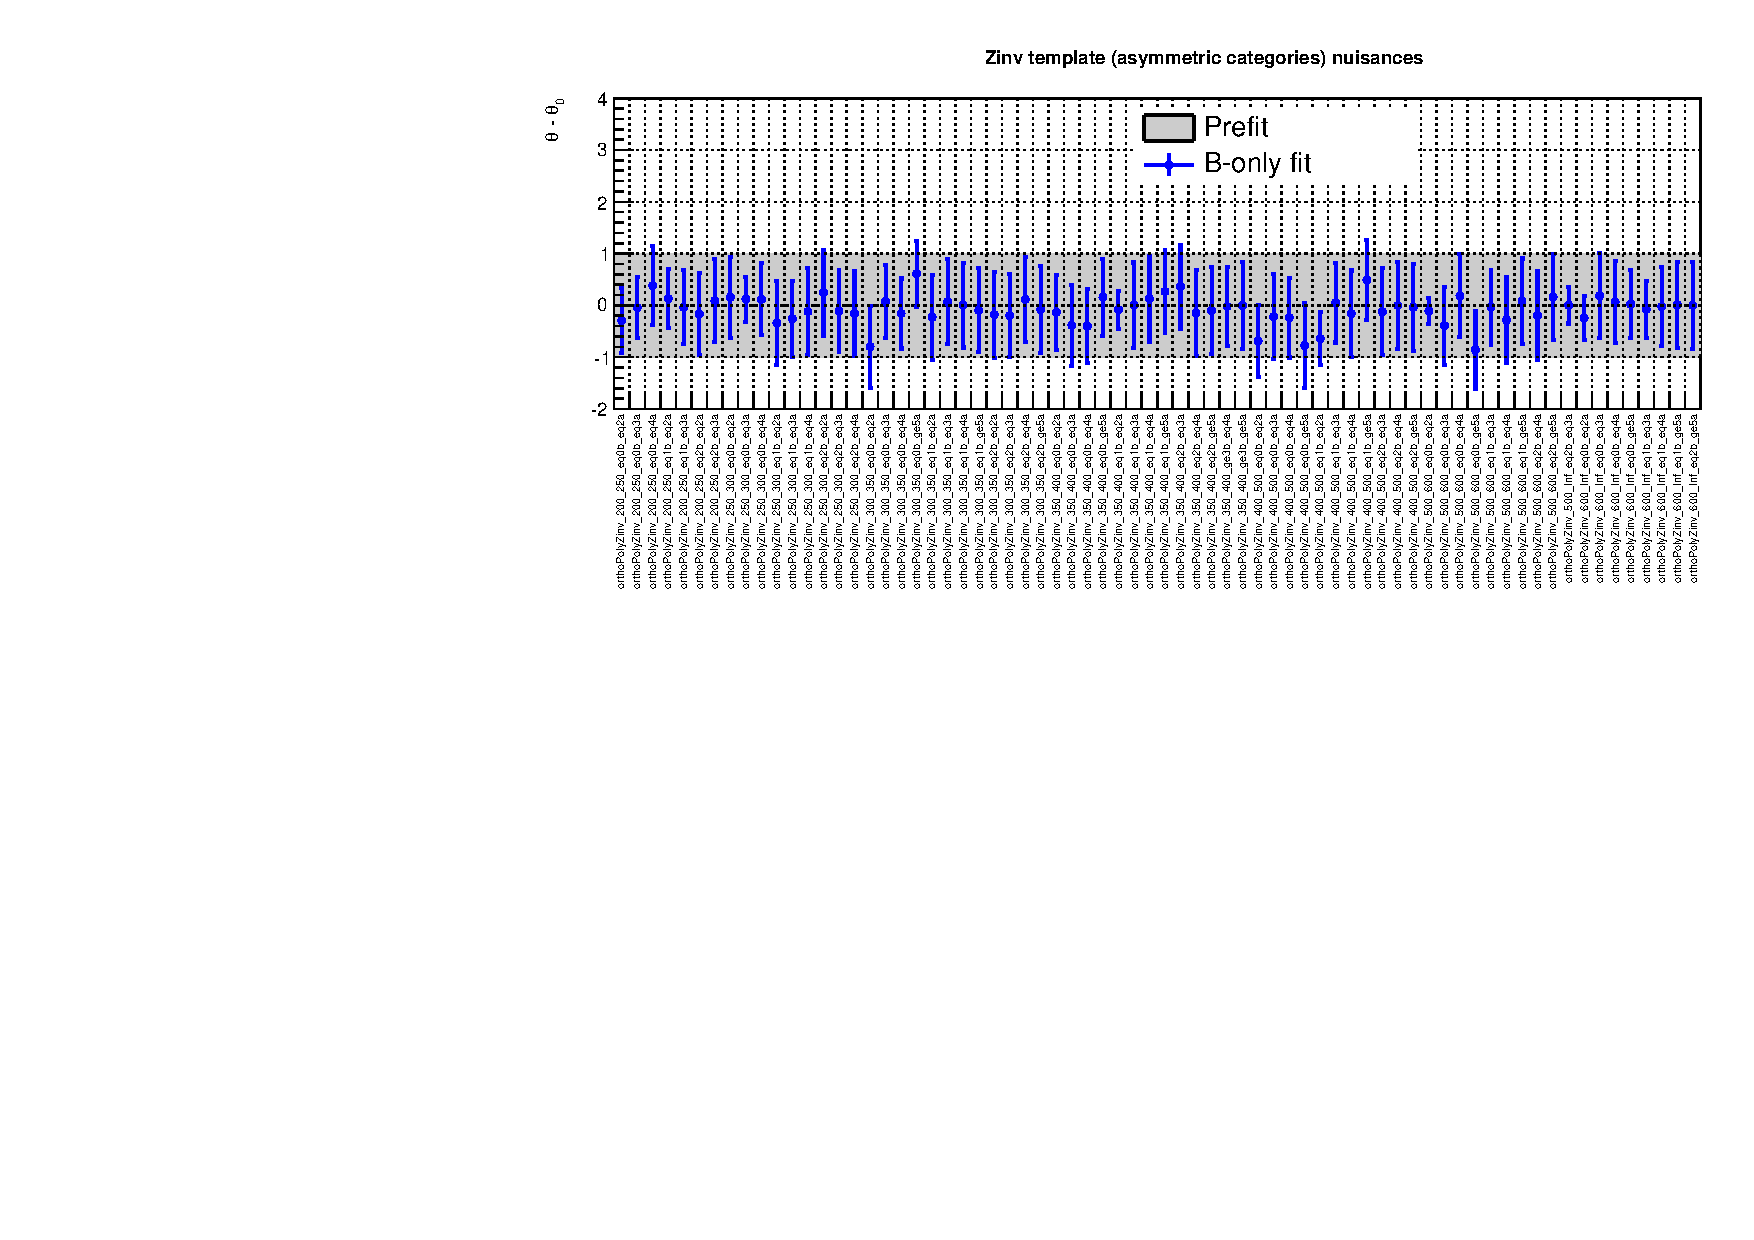
\includegraphics[width=0.8\textwidth]{figures/postFitResults/nuisancePlots/TemplateZinv_asym_nuisances} } \\
    \subfigure[Symmetric categories]{ 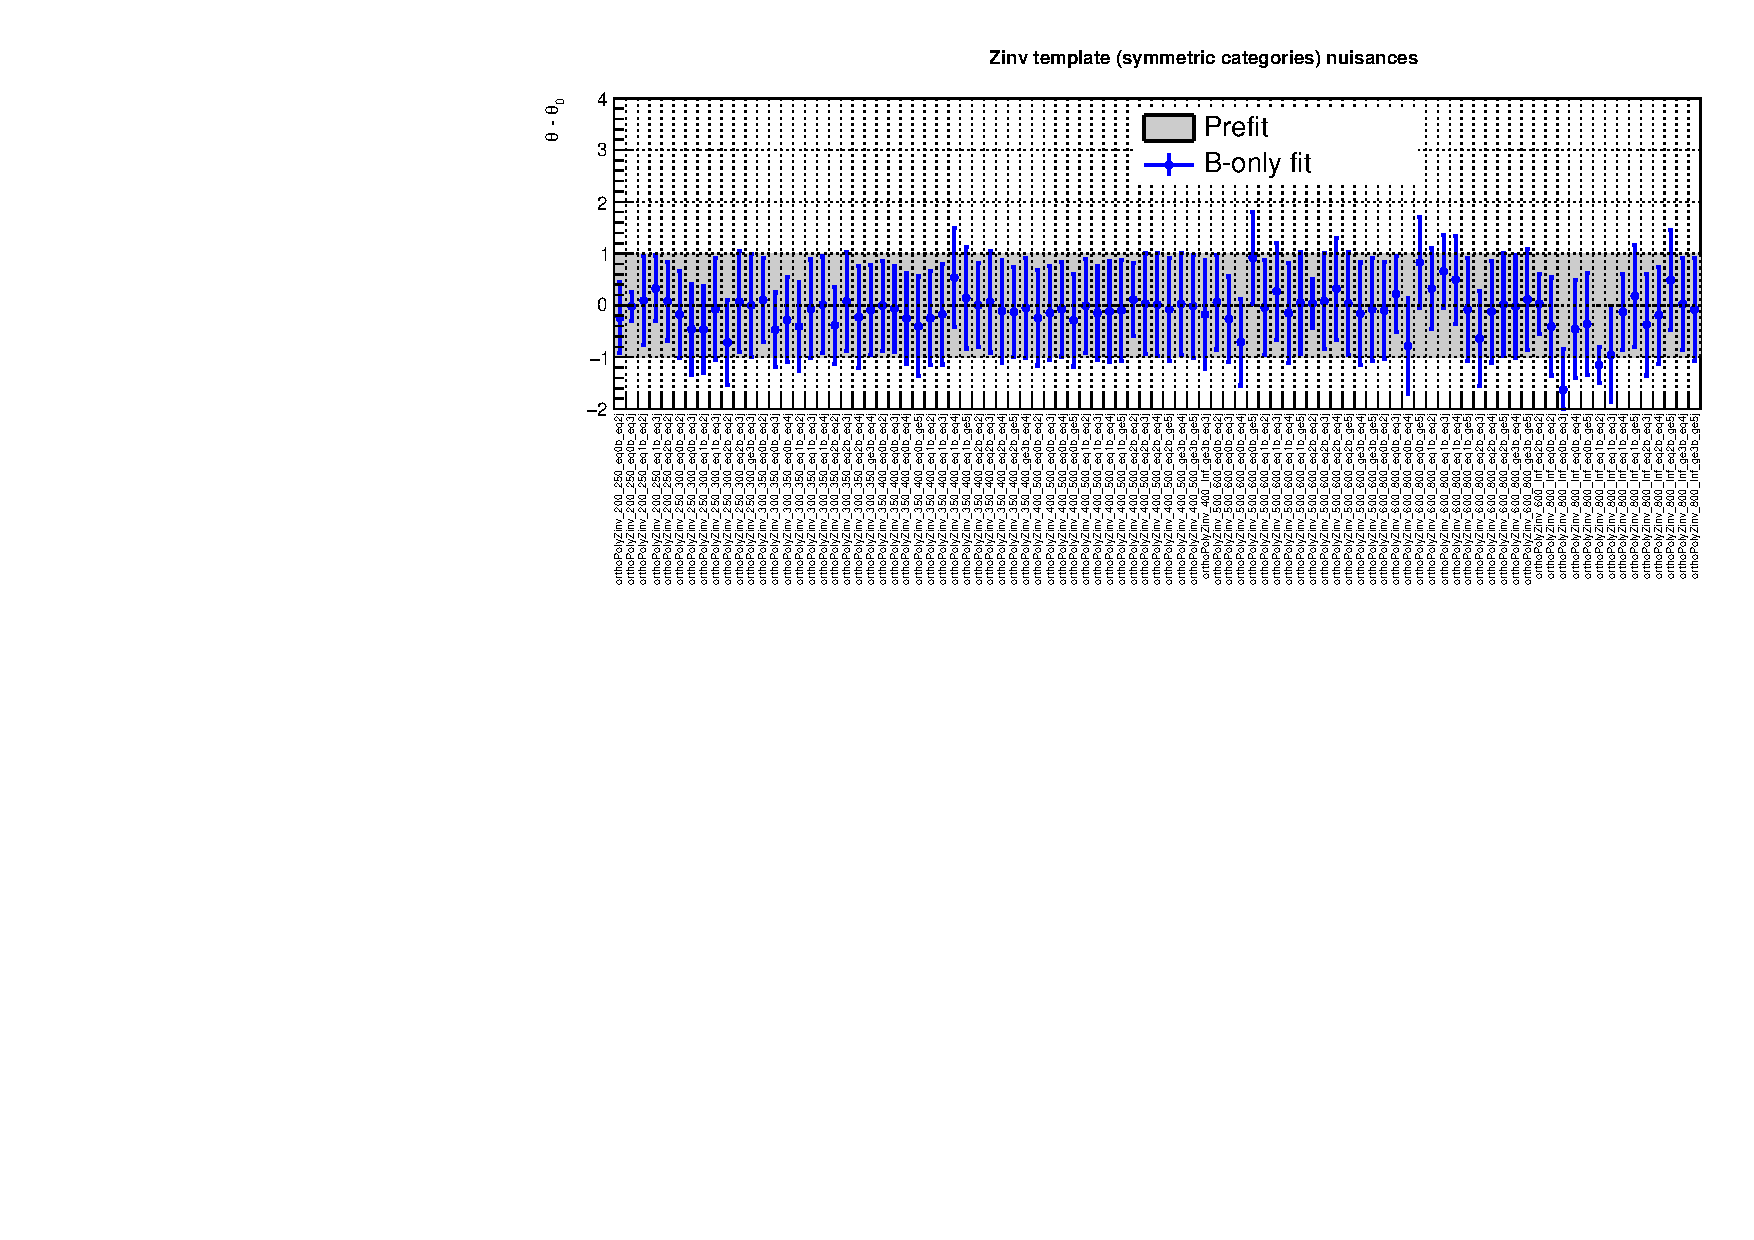
\includegraphics[width=0.8\textwidth]{figures/postFitResults/nuisancePlots/TemplateZinv_sym_nuisances} }
  \end{center}
\end{figure}


\begin{figure}[tbhp]
    \caption{ Pull of the nuisances parameters associated to the QCD systematic uncertainty, 
      for the asymmetric (symmetric) categories on the left (right).
      \label{fig:nuisPull_qcd}}
  \begin{center}
    \subfigure[Asymmetric categories]{ 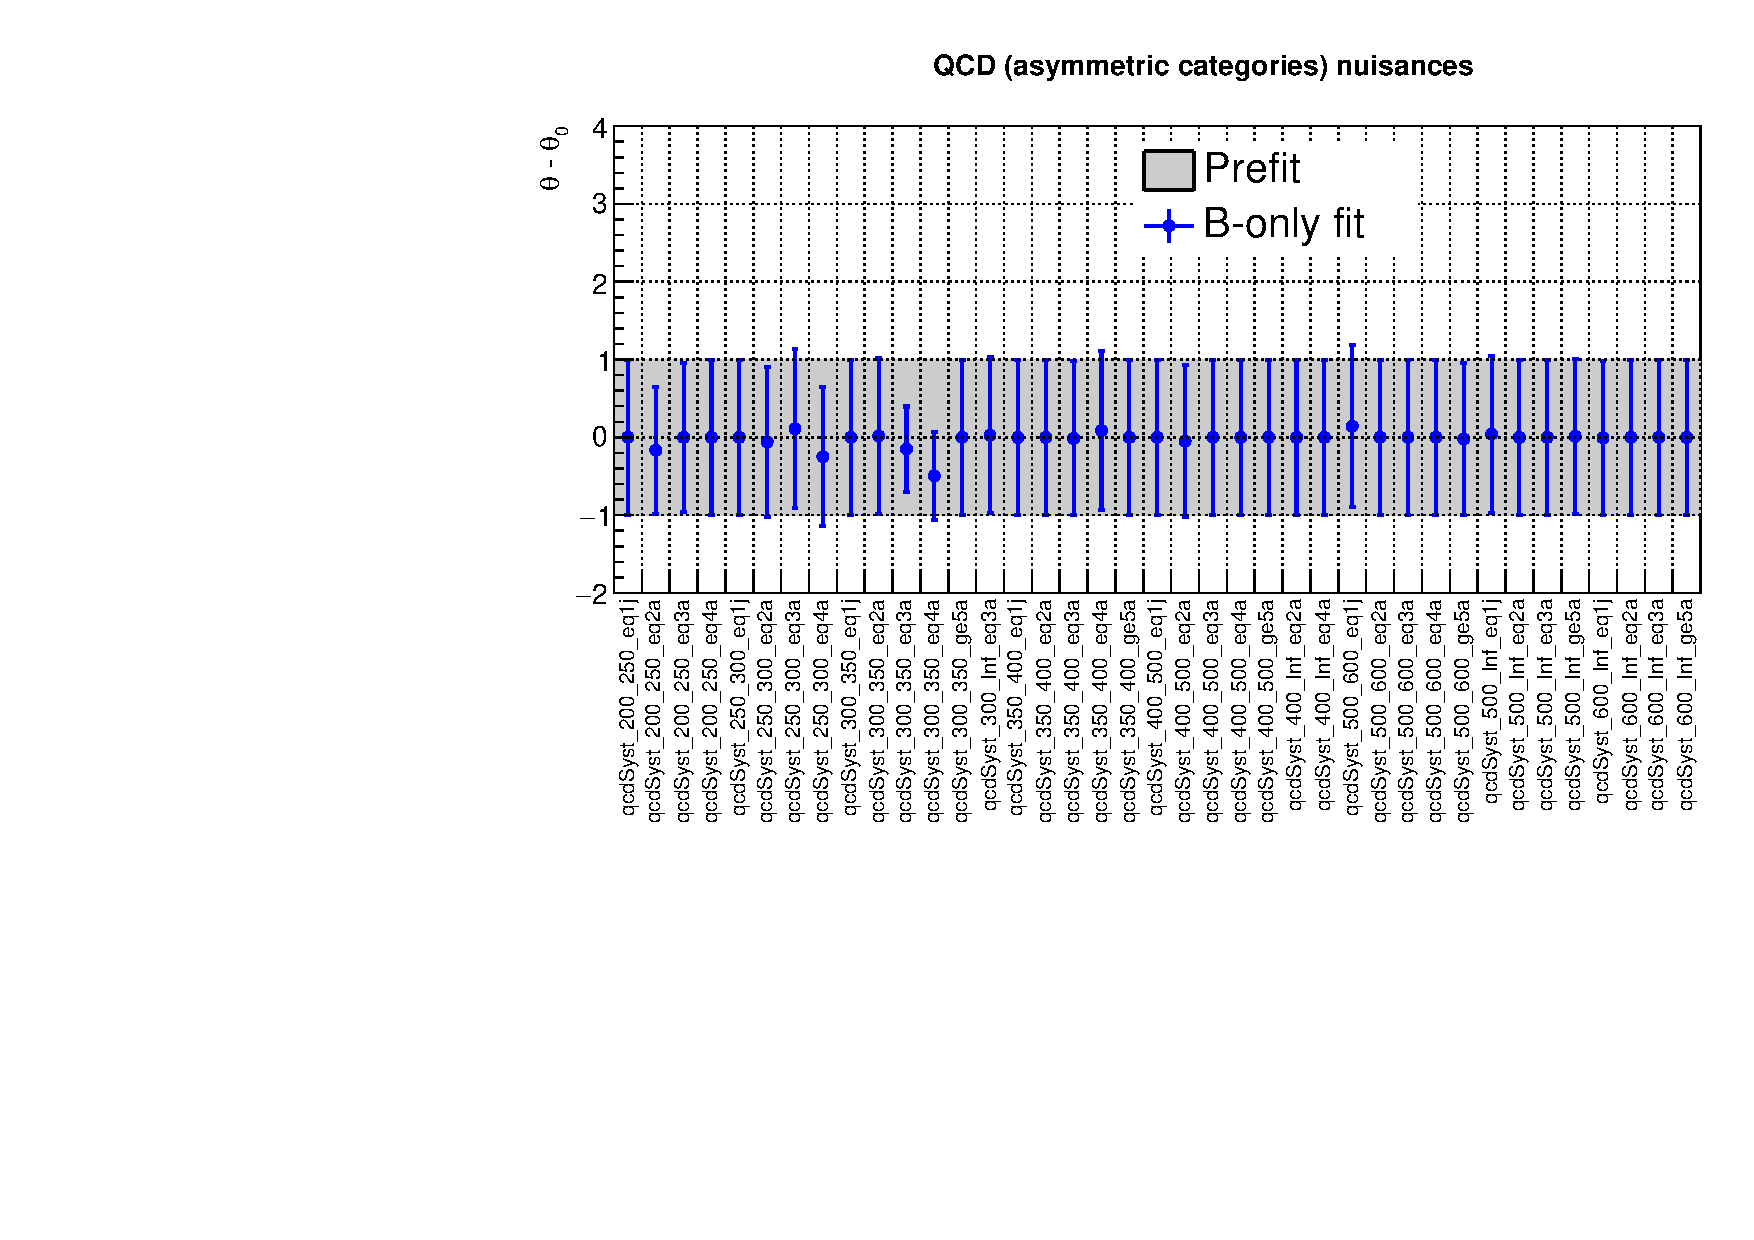
\includegraphics[width=0.45\textwidth]{figures/postFitResults/nuisancePlots/qcd_asym_nuisances} } ~~
    \subfigure[Symmetric categories]{ 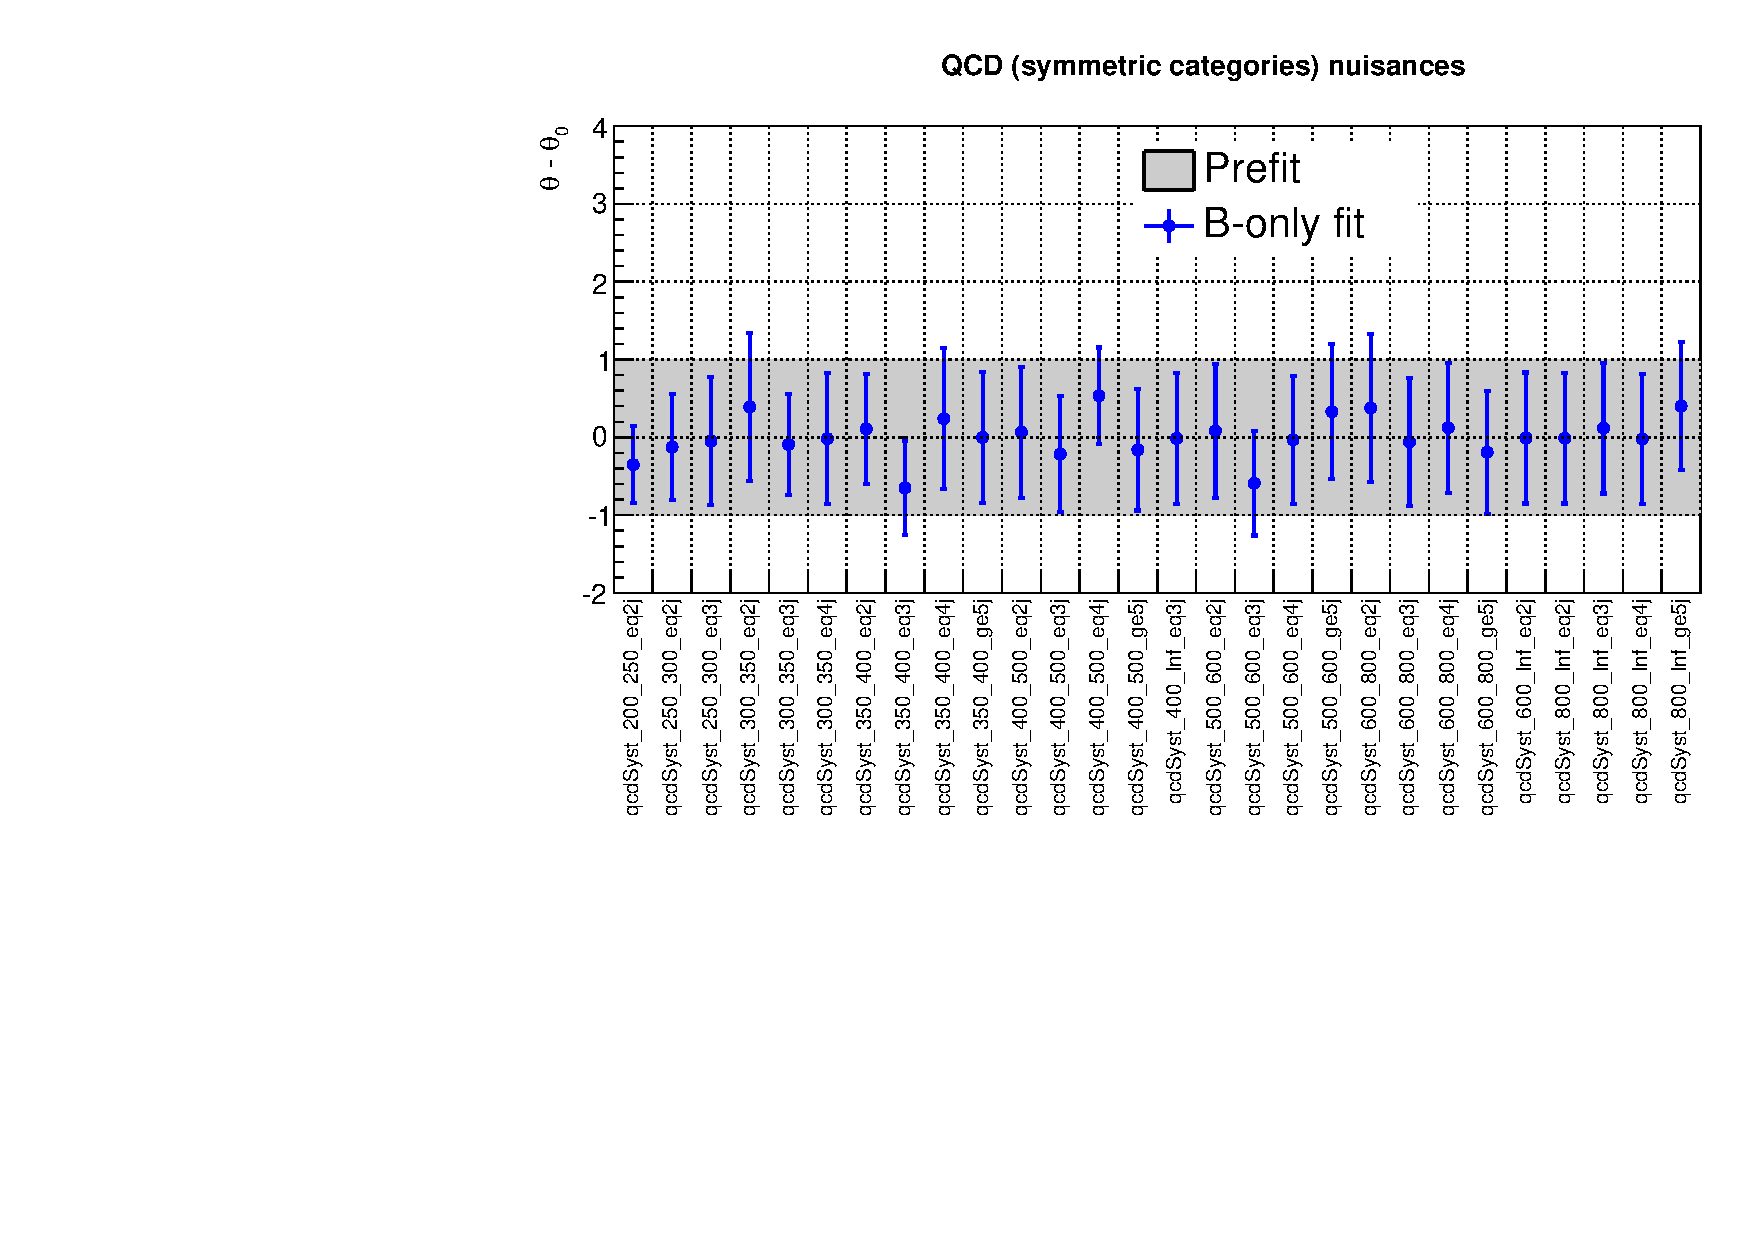
\includegraphics[width=0.45\textwidth]{figures/postFitResults/nuisancePlots/qcd_sym_nuisances} }
  \end{center}
\end{figure}


\begin{figure}[tbhp]
    \caption{ Pull of the nuisances parameters associated to the correlated systematic uncertainties. 
      \label{fig:nuisPull_Correlated}}
  \begin{center}
    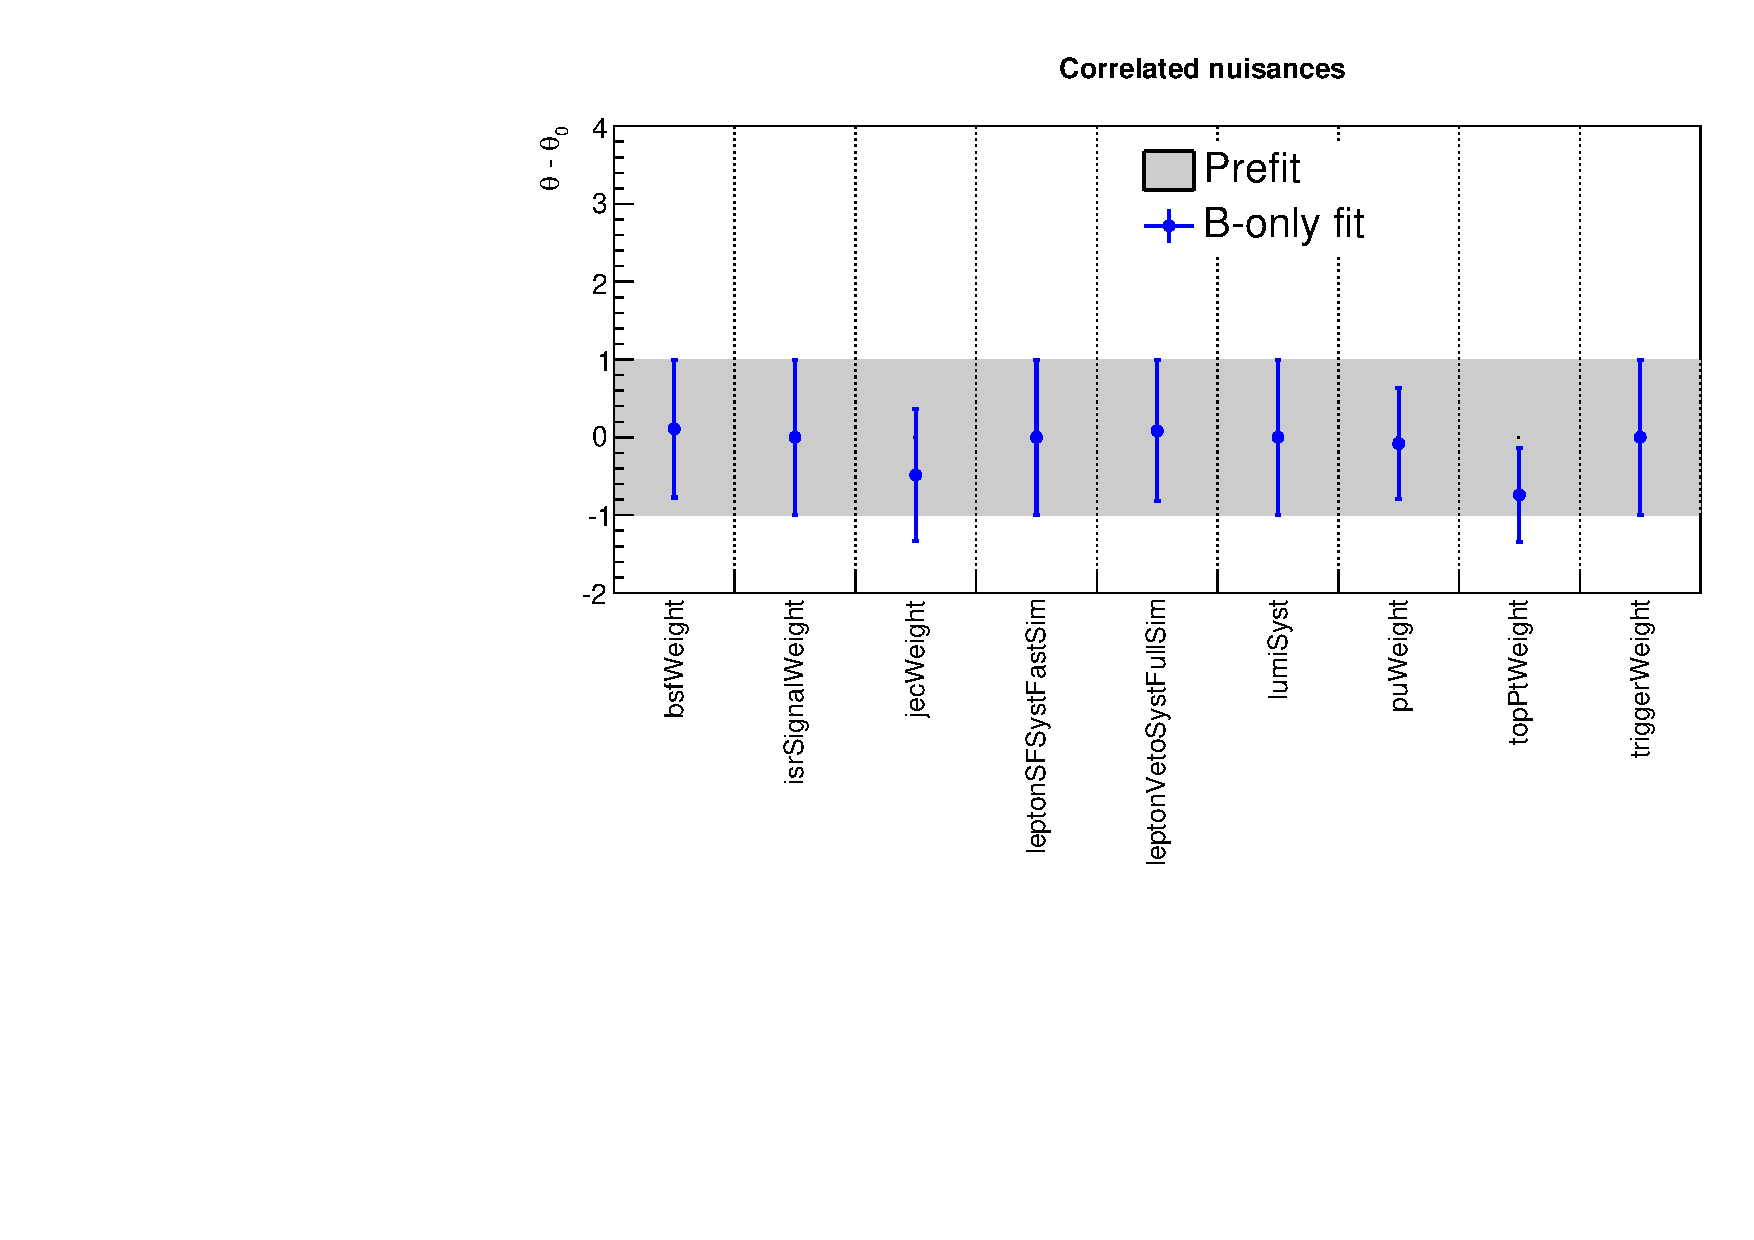
\includegraphics[width=0.8\textwidth]{figures/postFitResults/nuisancePlots/Correlated_nuisances}
  \end{center}
\end{figure}

\clearpage

%% \begin{figure}[tbhp]
%%     \begin{center}
%%         \subfigure[Symmetric Uncorrected]{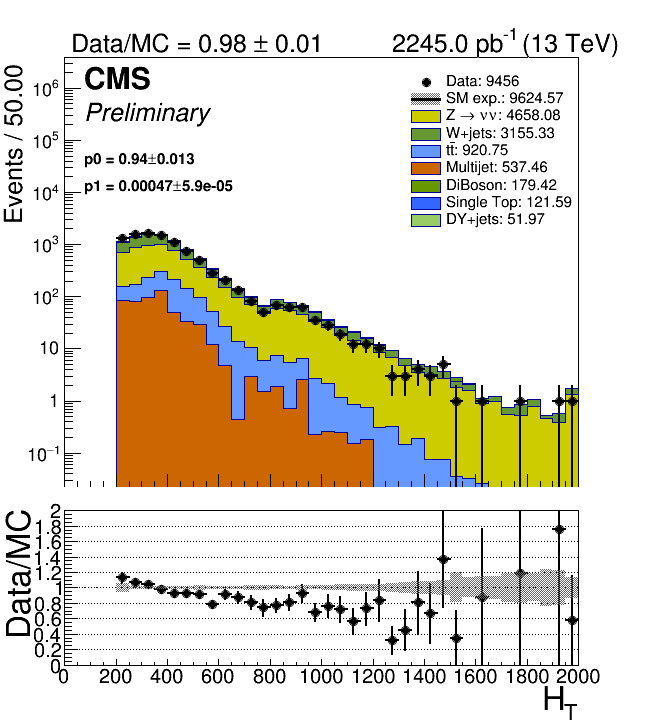
\includegraphics[width=0.38\textwidth]{figures/uncorrectedShapes/sym/all/ht40_sym_all}} ~~
%%         \subfigure[Symmetric Corrected] {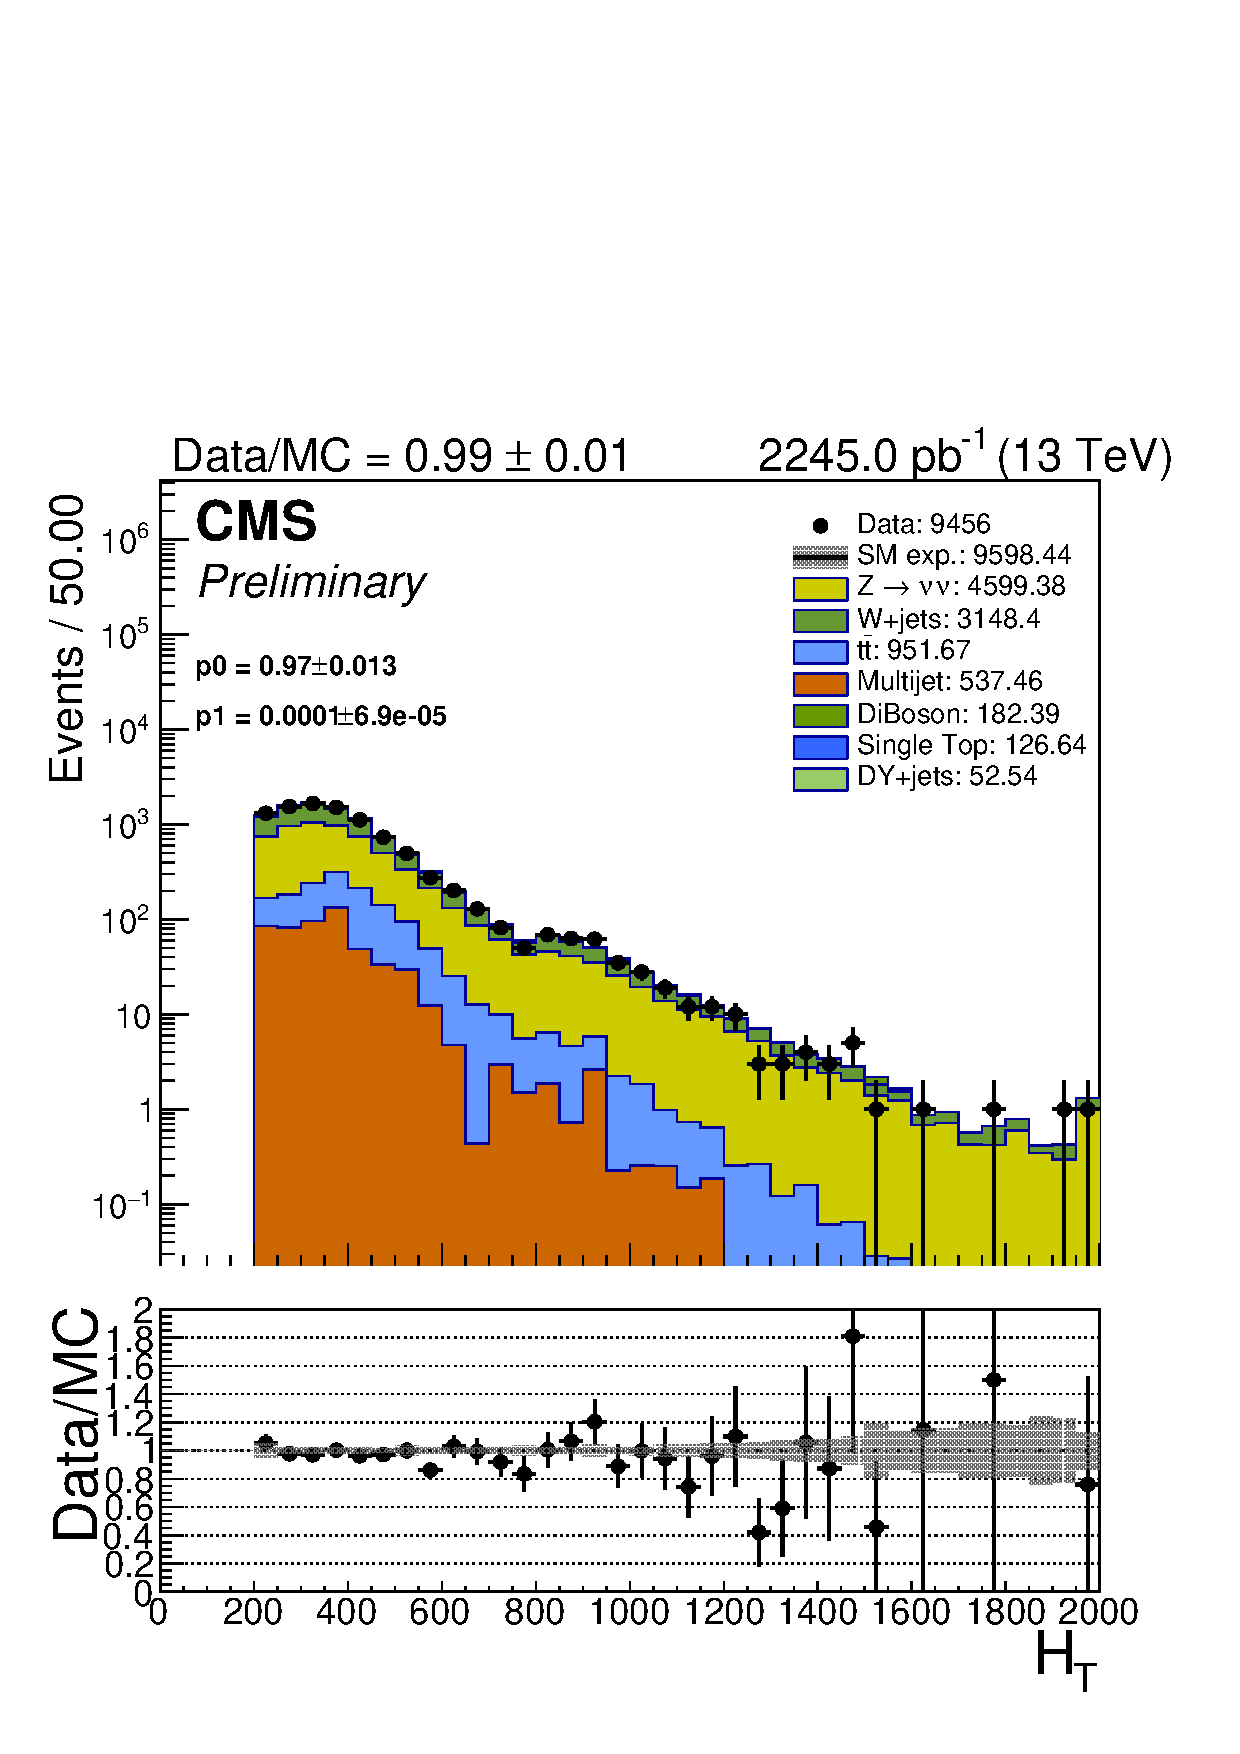
\includegraphics[width=0.38\textwidth]{figures/correctedShapes/sym/all/ht40_sym_all}}\\
%%         \subfigure[Asymmetric Uncorrected] {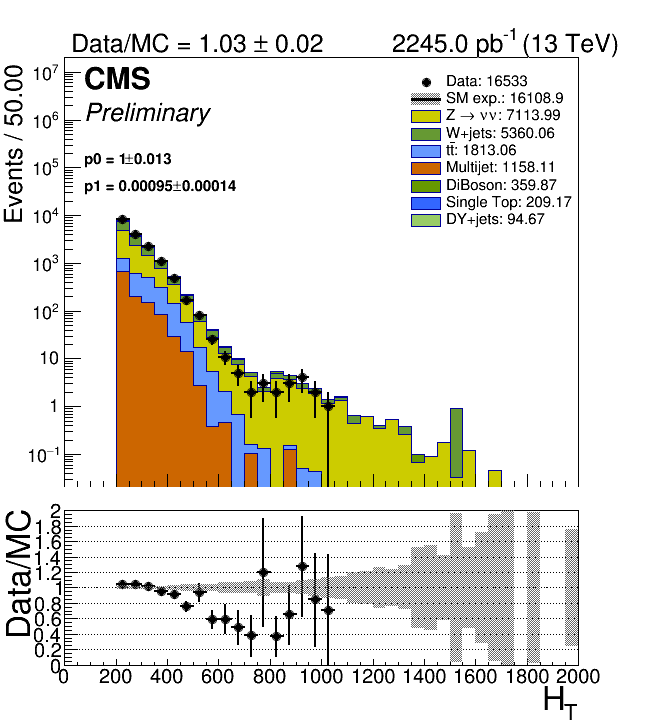
\includegraphics[width=0.38\textwidth]{figures/uncorrectedShapes/asym/all/ht40_asym_all}} ~~
%%         \subfigure[Asymmetric Corrected] {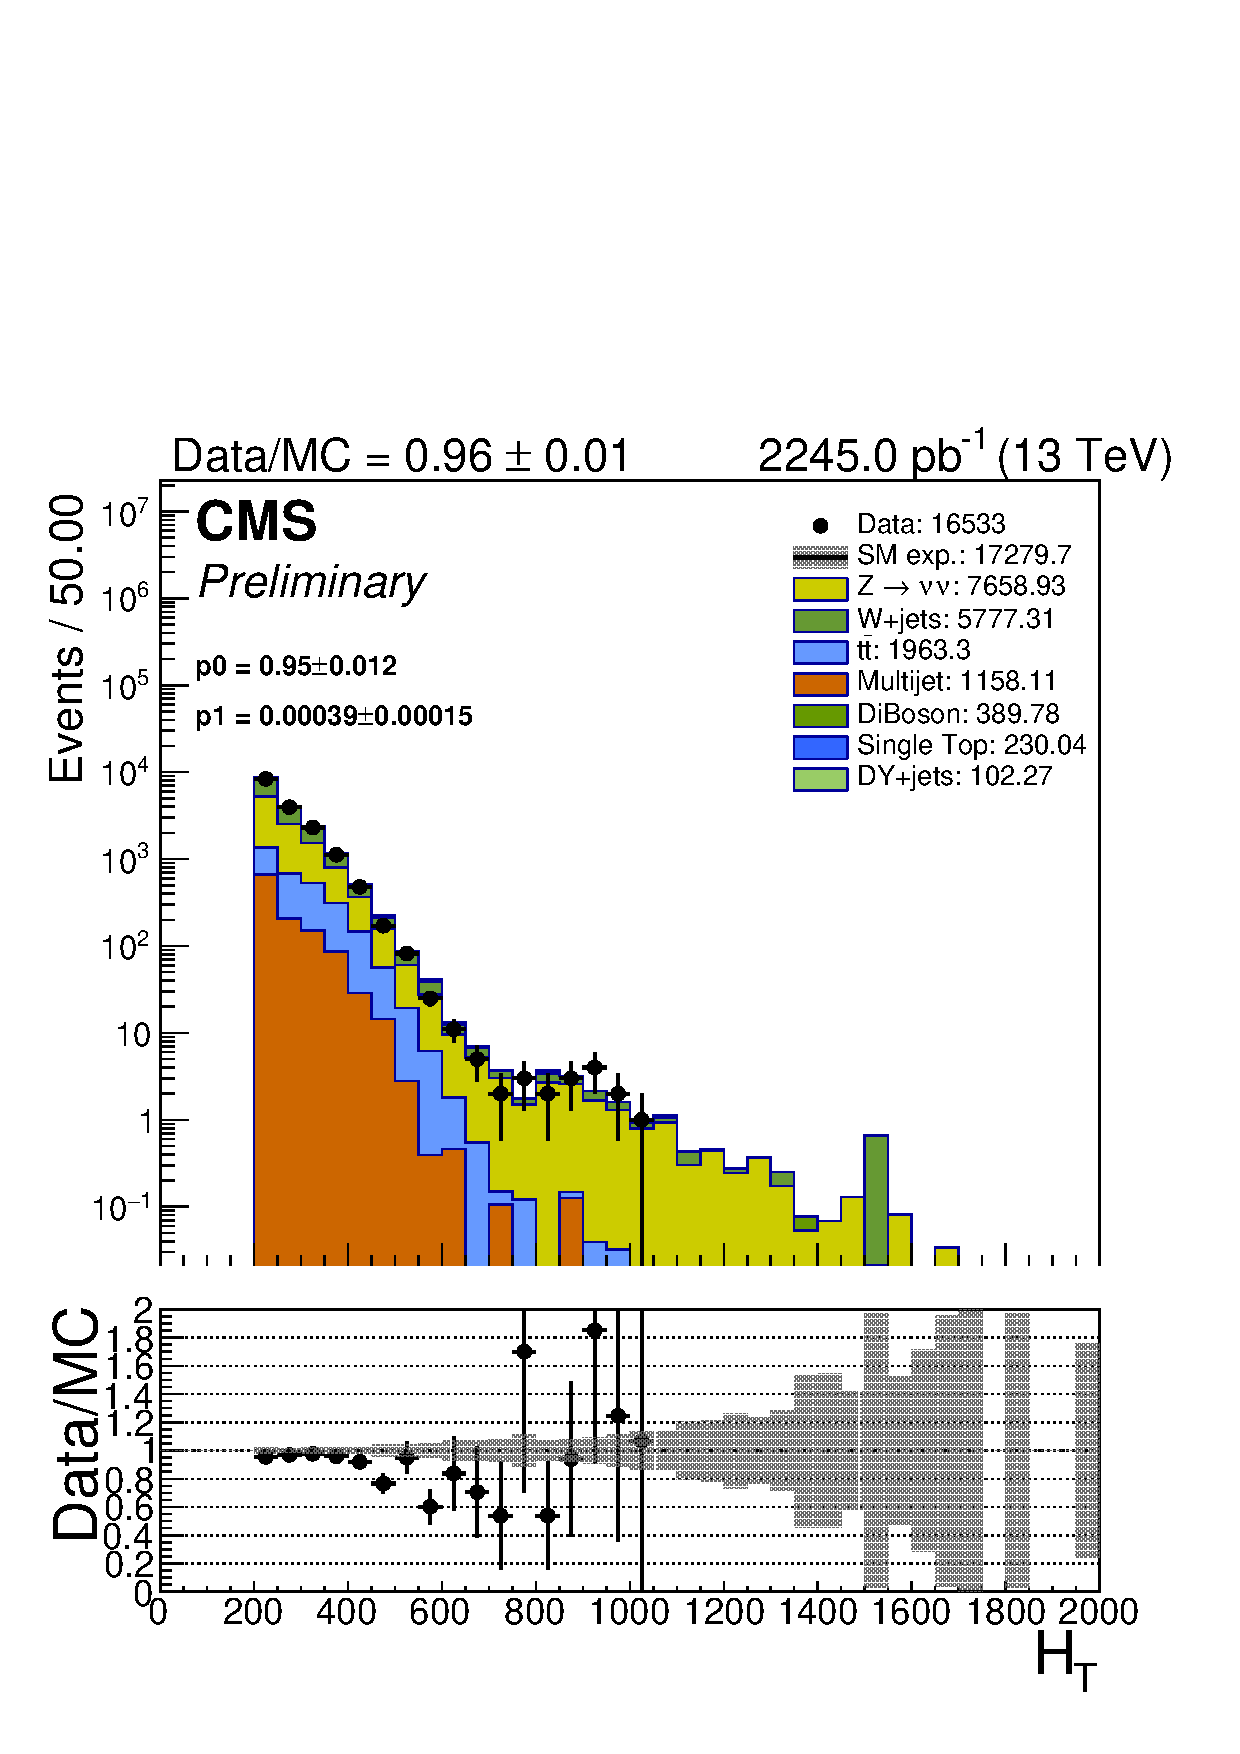
\includegraphics[width=0.38\textwidth]{figures/correctedShapes/asym/all/ht40_asym_all}}\\
%%         \subfigure[Monojet Unorrected] {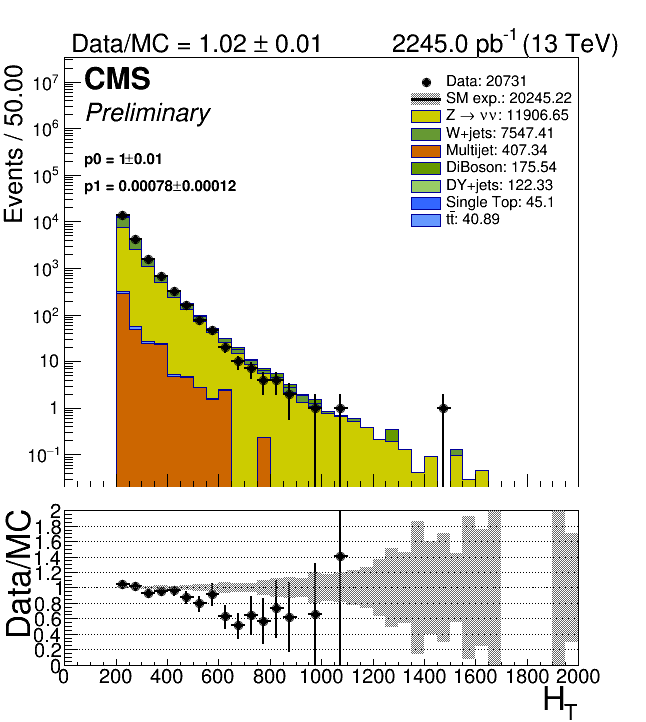
\includegraphics[width=0.38\textwidth]{figures/uncorrectedShapes/mono/all/ht40_mono_all}} ~~
%%         \subfigure[Monojet Corrected]{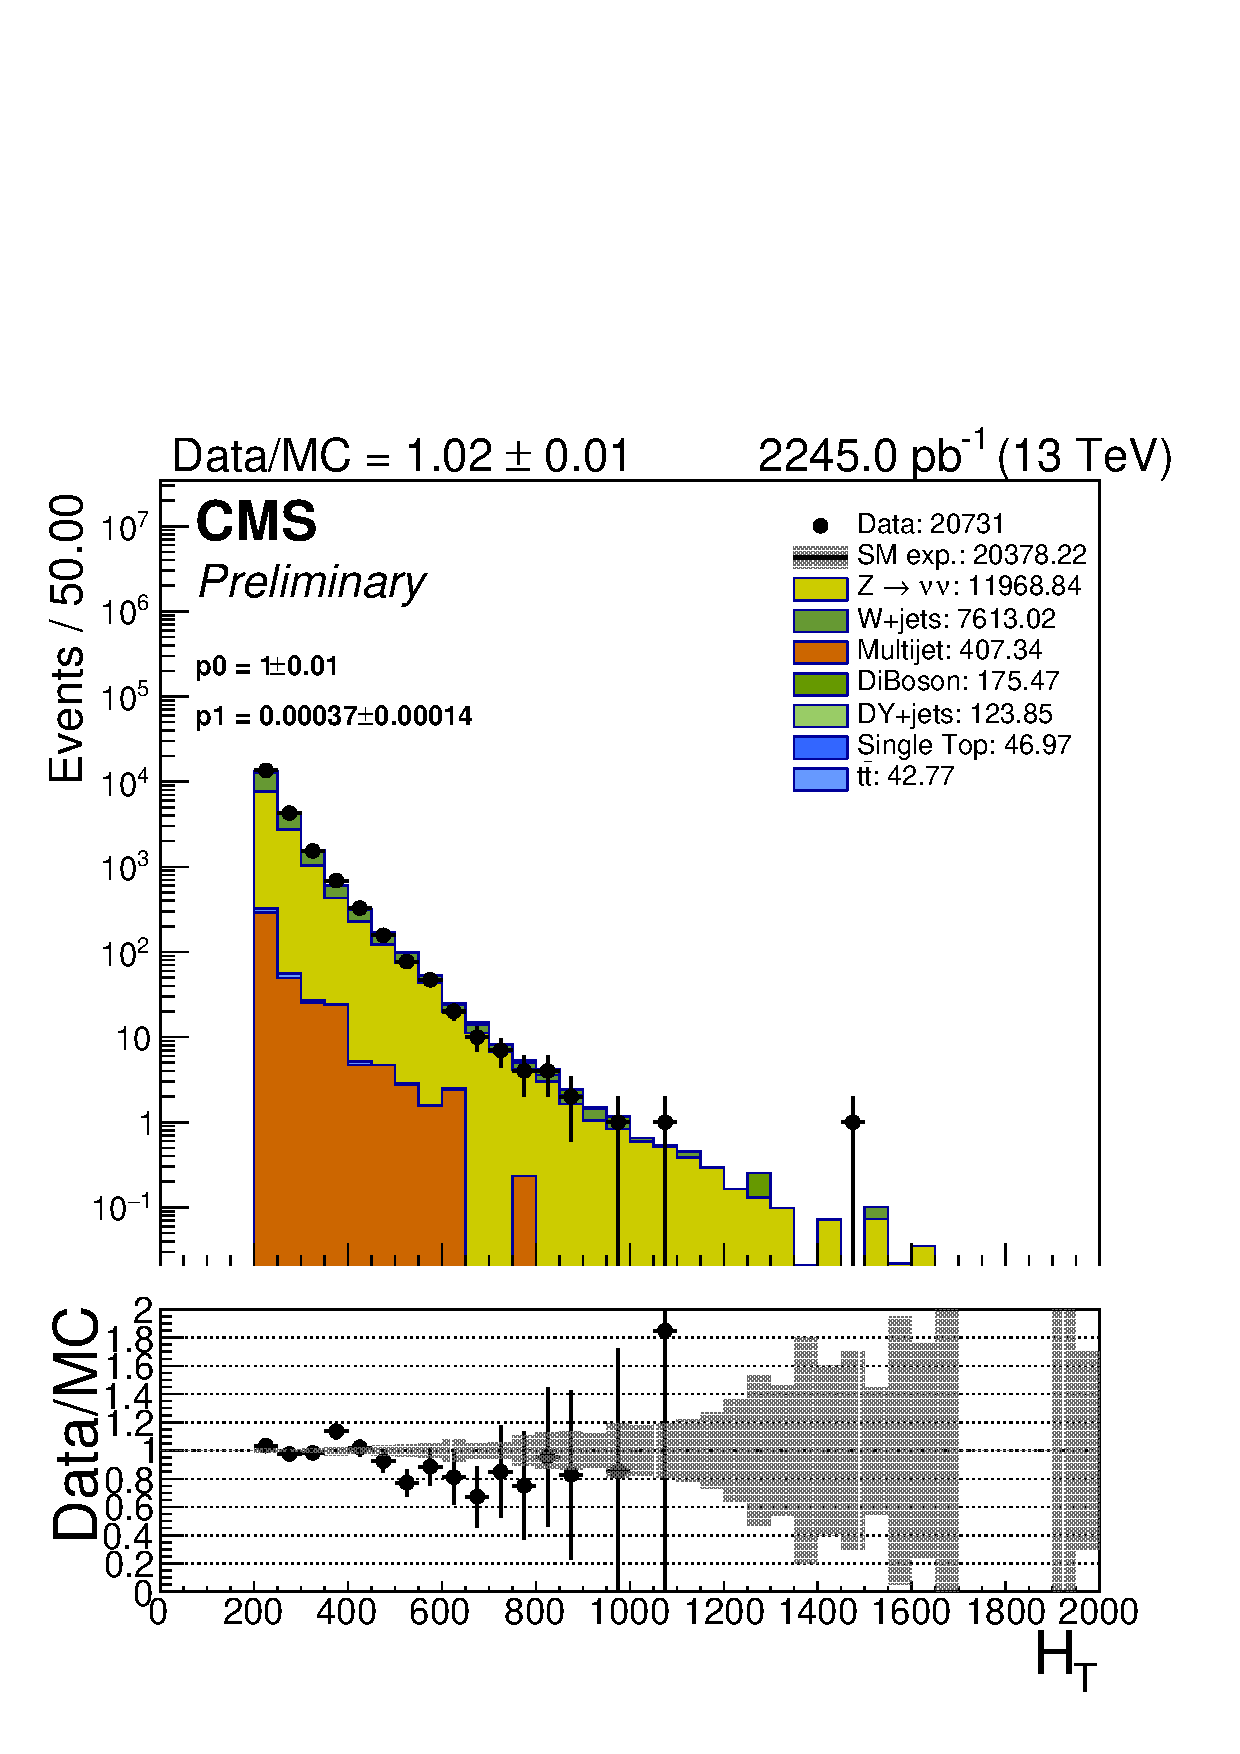
\includegraphics[width=0.38\textwidth]{figures/correctedShapes/mono/all/ht40_mono_all}}\\
%%         \caption{The \scalht distribution comparing data and prediction agreement before and after applying the correction from the control region only fit. Also shown are the results of a linear fit to the data/prediction ratio (p0,p1 parameters) which confirms the agreeement is significantly improved through the correction applied in the control regions}
%%         \label{fig:shapesht}
%%     \end{center}
%% \end{figure}

%% \begin{figure}[tbhp]
%%     \begin{center}
%%         \subfigure[Symmetric Uncorrected]{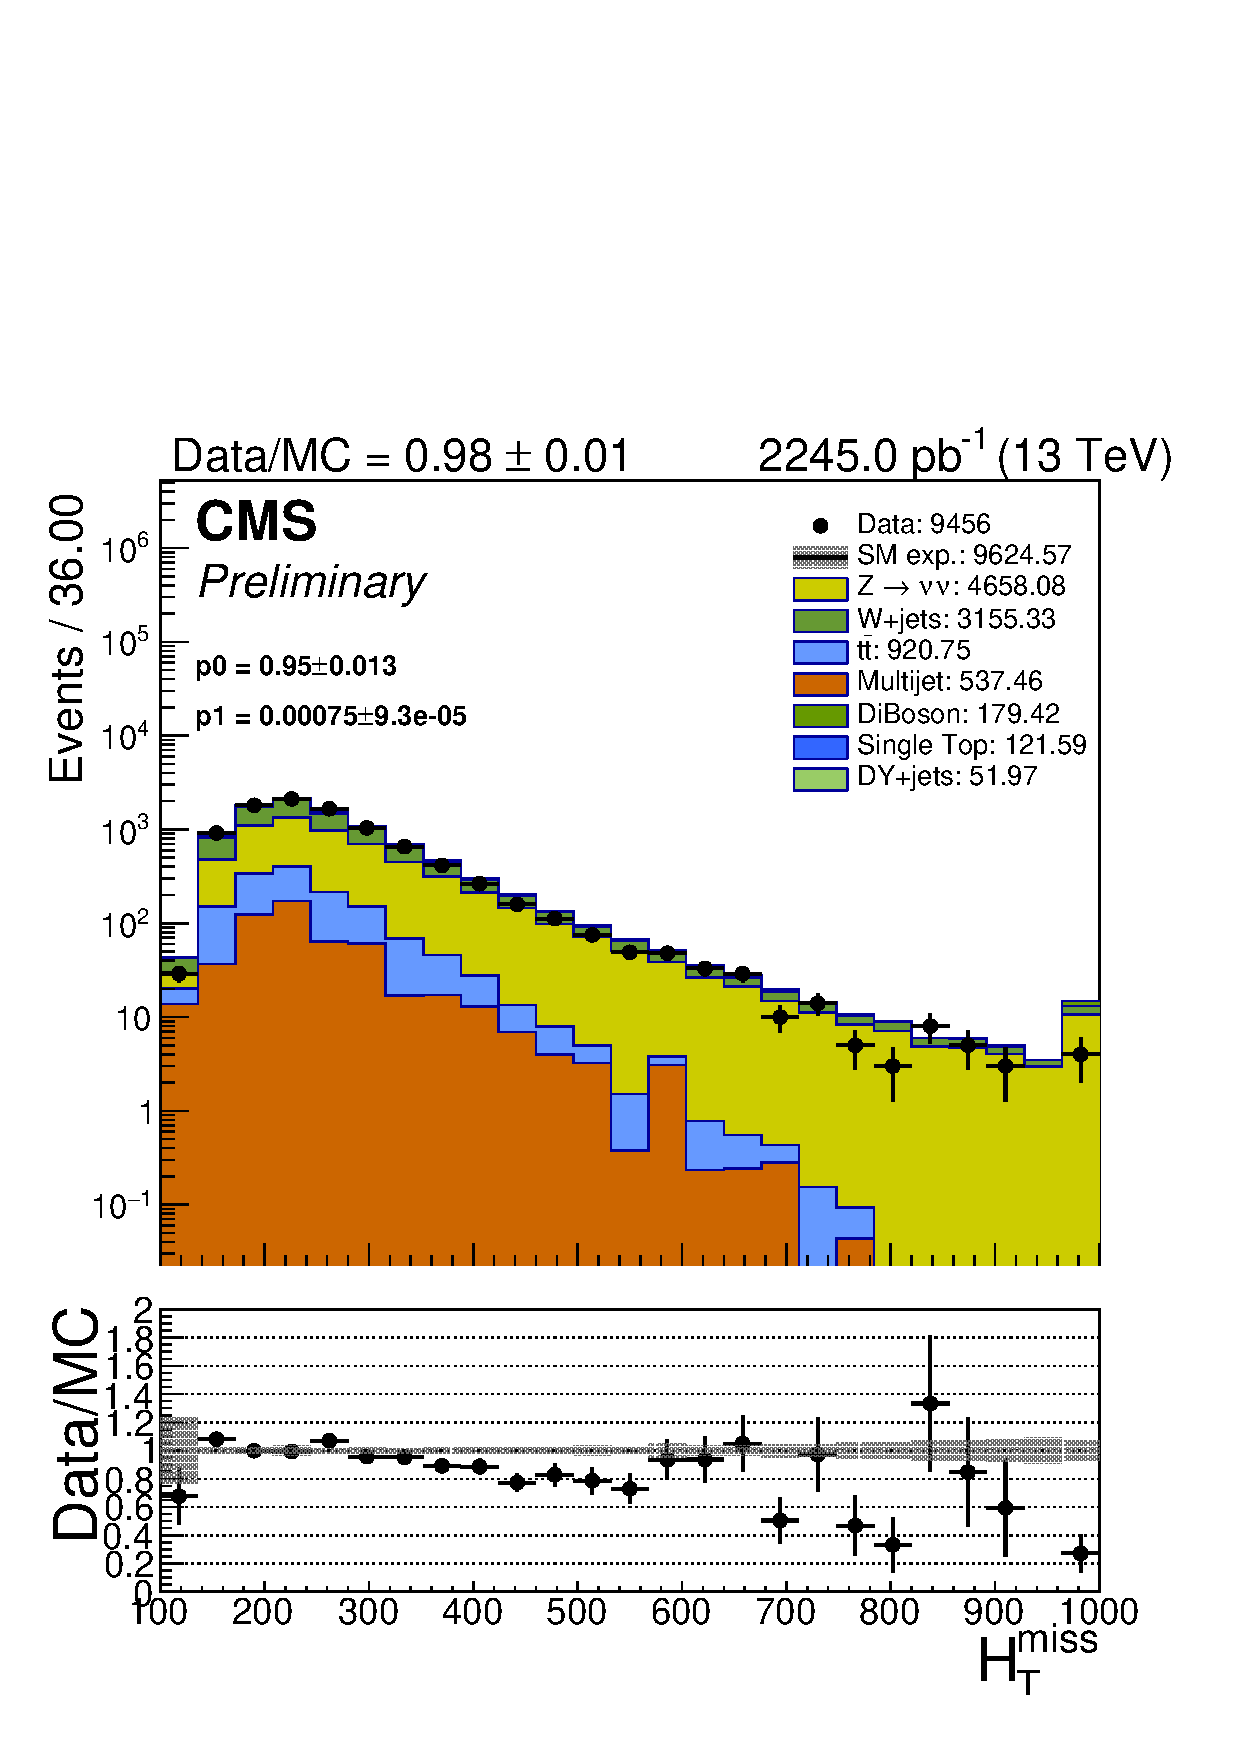
\includegraphics[width=0.38\textwidth]{figures/uncorrectedShapes/sym/all/mht40_pt_sym_all}} ~~
%%         \subfigure[Symmetric Corrected] {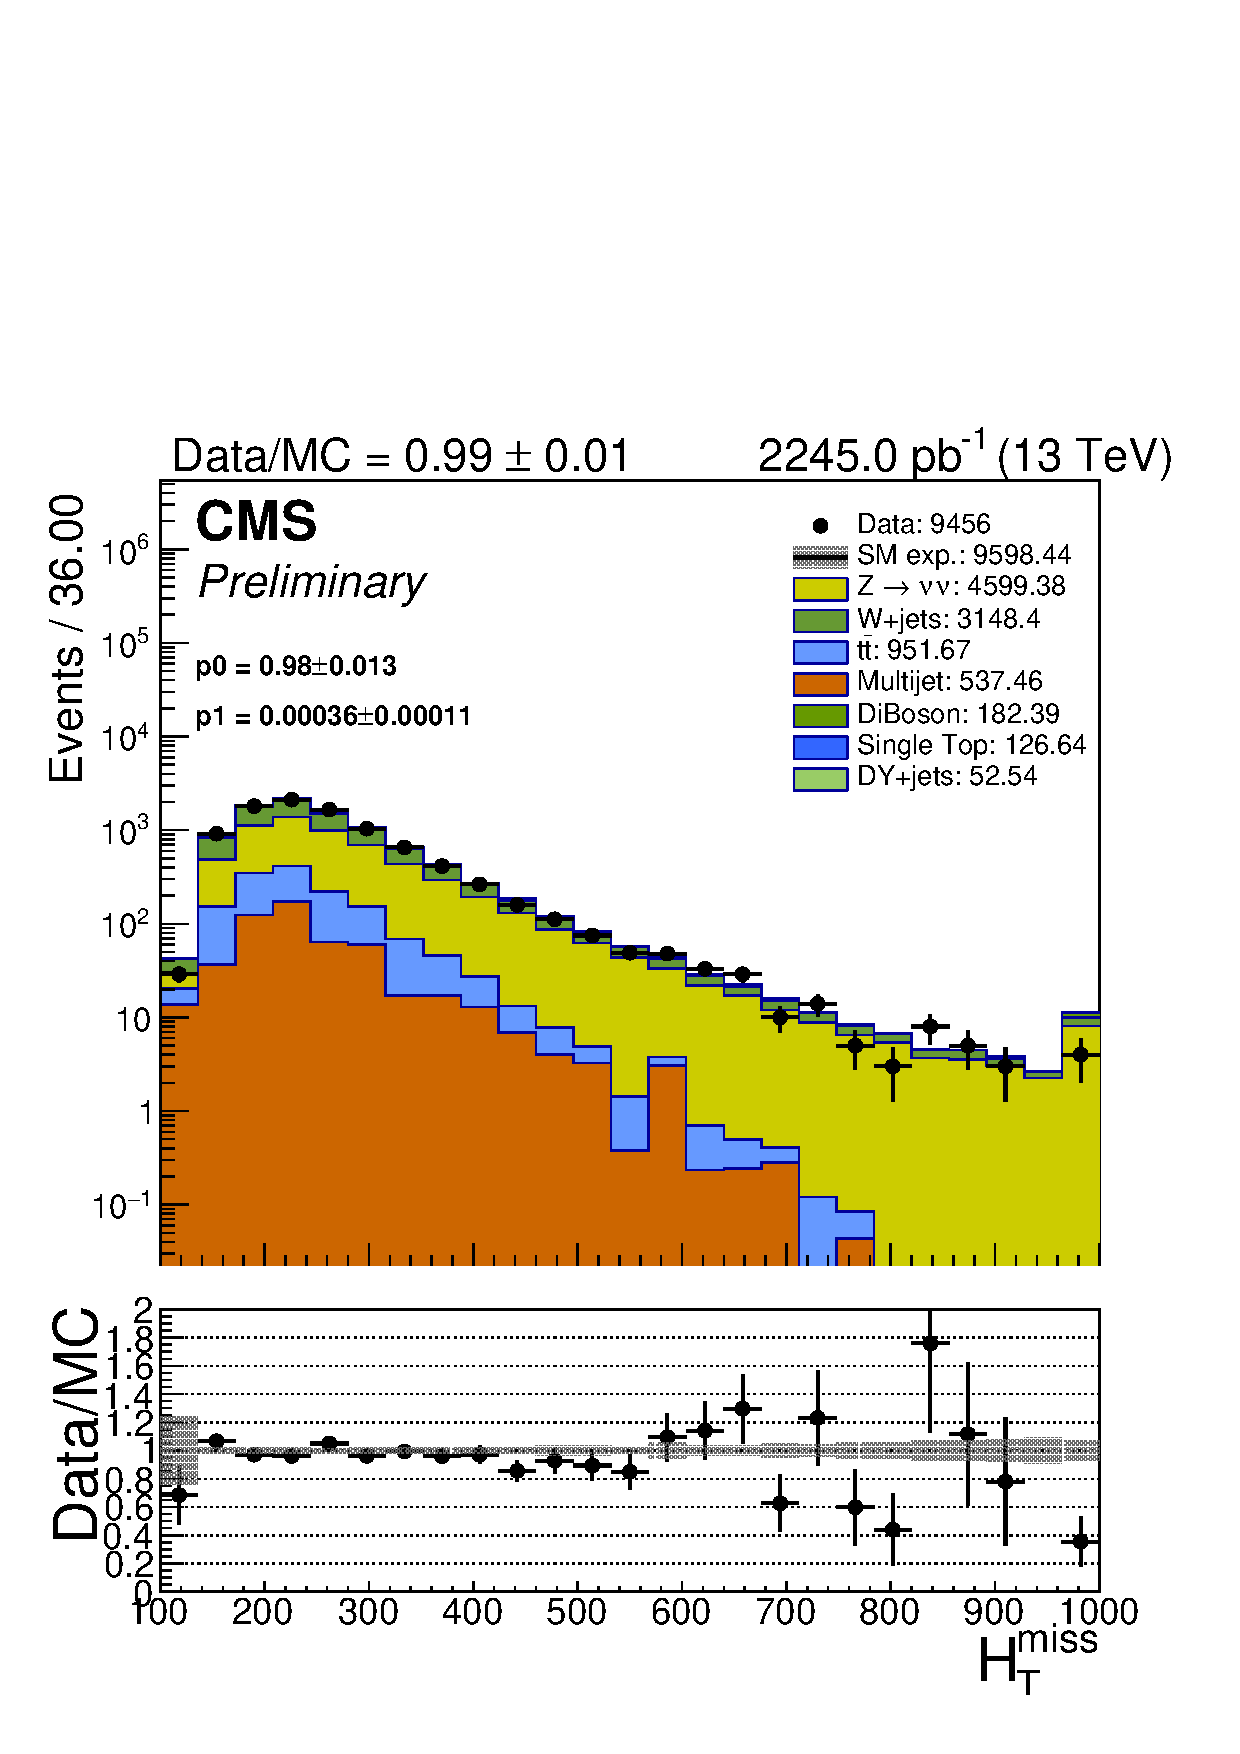
\includegraphics[width=0.38\textwidth]{figures/correctedShapes/sym/all/mht40_pt_sym_all}}\\
%%         \subfigure[Asymmetric Uncorrected] {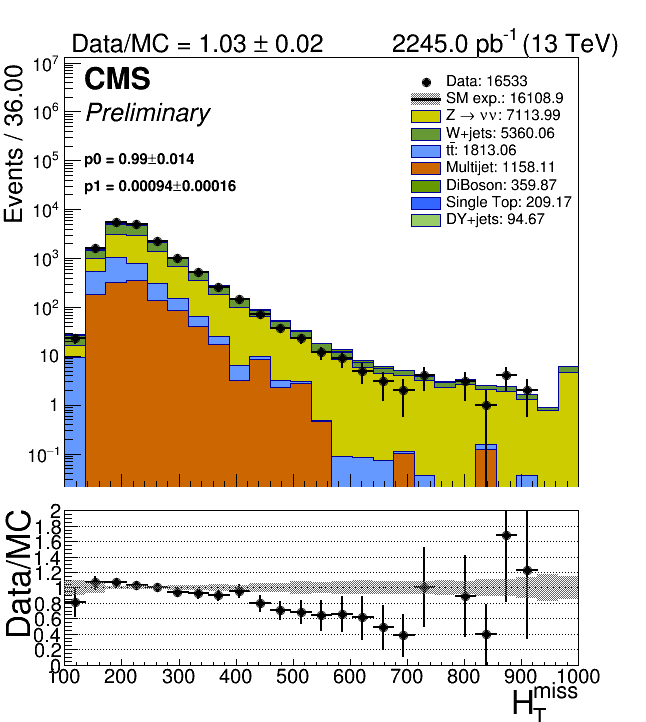
\includegraphics[width=0.38\textwidth]{figures/uncorrectedShapes/asym/all/mht40_pt_asym_all}} ~~
%%         \subfigure[Asymmetric Corrected] {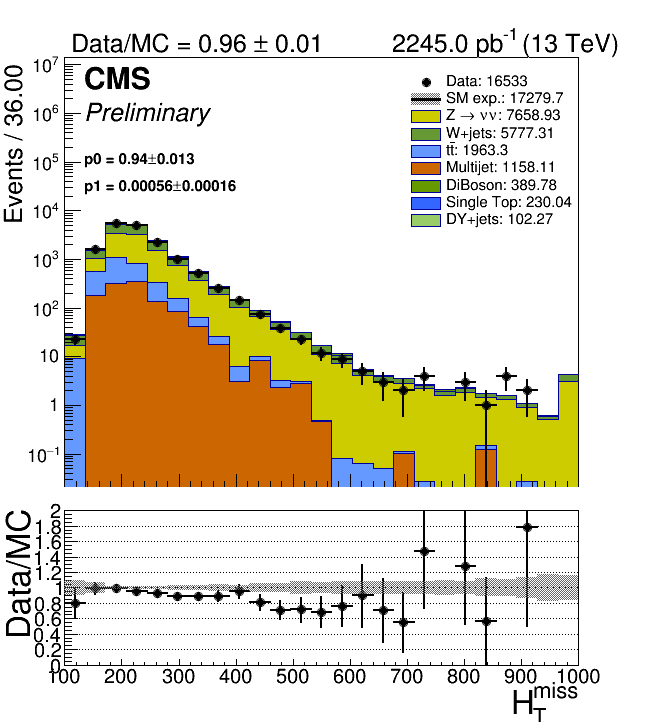
\includegraphics[width=0.38\textwidth]{figures/correctedShapes/asym/all/mht40_pt_asym_all}}\\
%%         \subfigure[Monojet Unorrected] {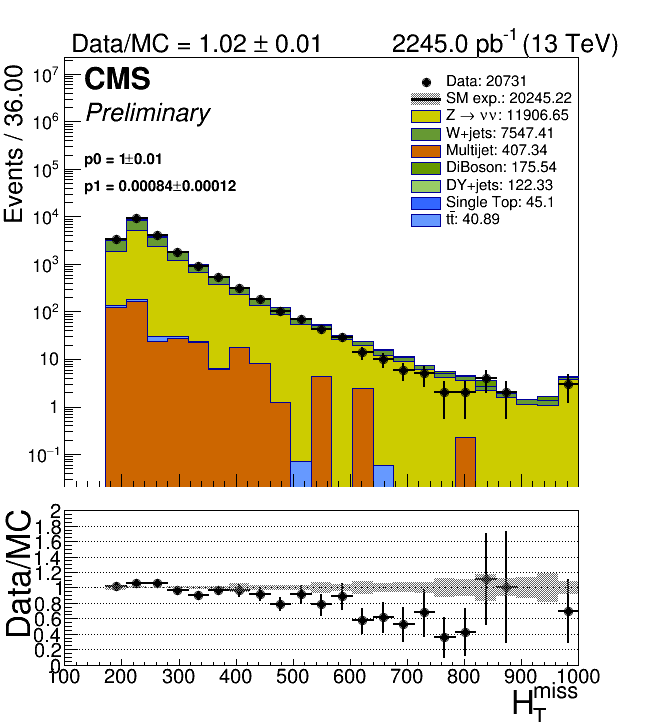
\includegraphics[width=0.38\textwidth]{figures/uncorrectedShapes/mono/all/mht40_pt_mono_all}} ~~
%%         \subfigure[Monojet Corrected]{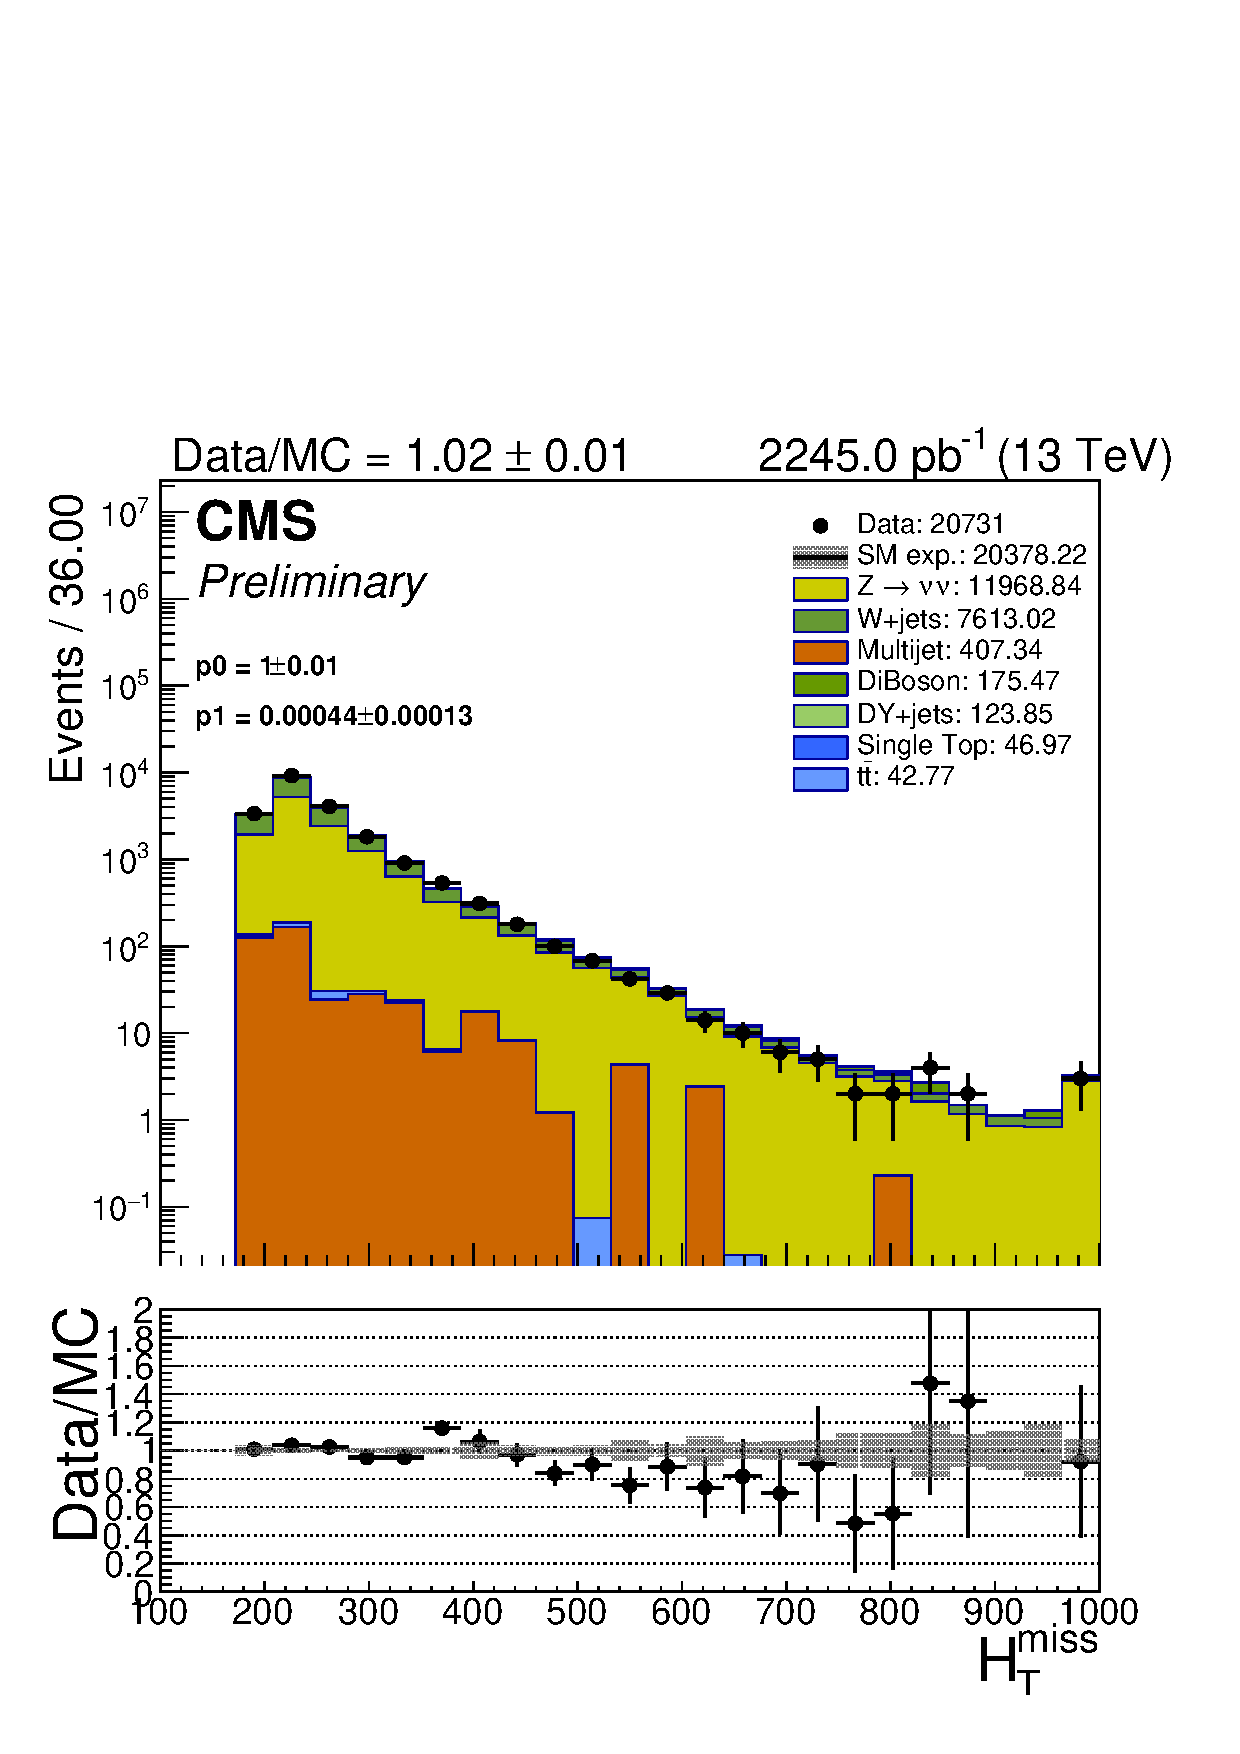
\includegraphics[width=0.38\textwidth]{figures/correctedShapes/mono/all/mht40_pt_mono_all}}\\
%%         \caption{The \mht distribution comparing data and prediction agreement before and after applying the correction from the control region only fit. Also shown are the results of a linear fit to the data/prediction ratio (p0,p1 parameters) which confirms the agreeement is significantly improved through the correction applied in the control regions}
%%     \end{center}
%% \end{figure}
%% \begin{figure}[tbhp]
%%     \begin{center}
%%         \subfigure[Symmetric Uncorrected]{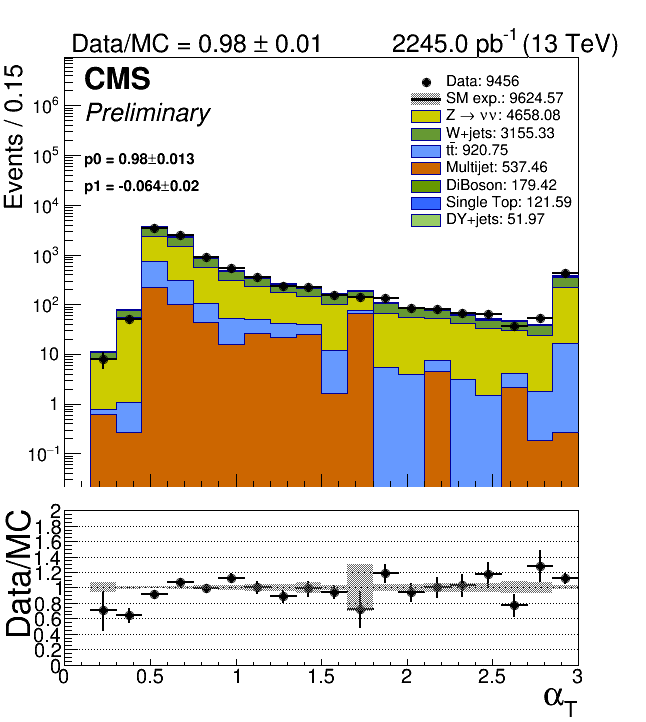
\includegraphics[width=0.38\textwidth]{figures/uncorrectedShapes/sym/all/alphaT_sym_all}} ~~
%%         \subfigure[Symmetric Corrected] {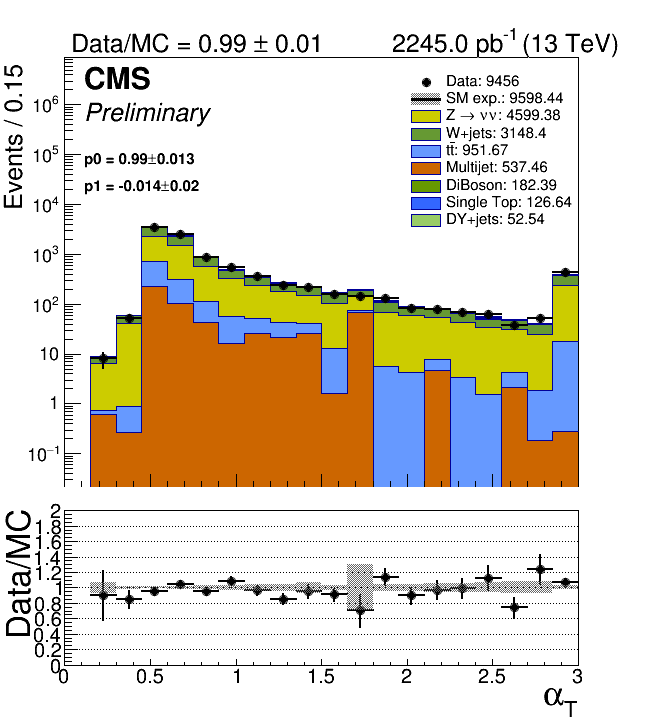
\includegraphics[width=0.38\textwidth]{figures/correctedShapes/sym/all/alphaT_sym_all}}\\
%%         \subfigure[Asymmetric Uncorrected] {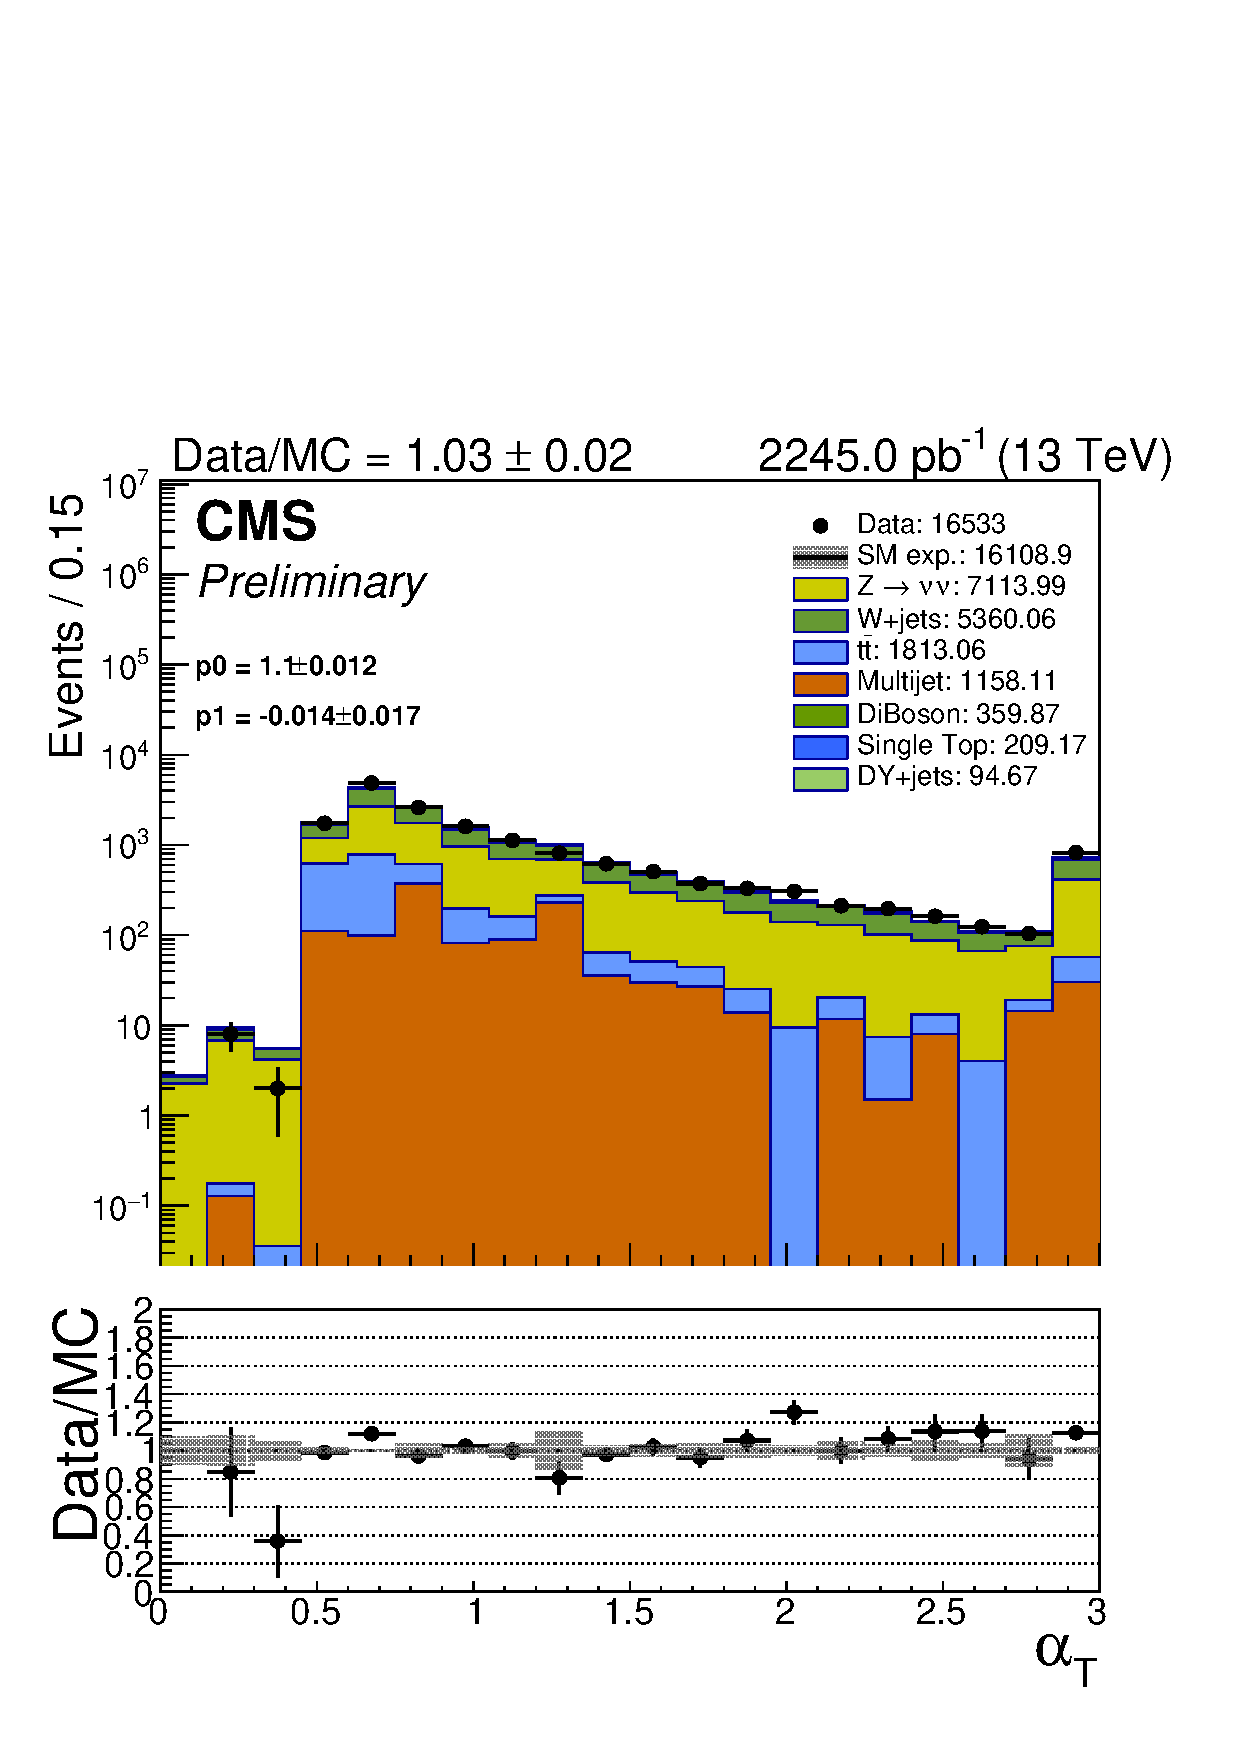
\includegraphics[width=0.38\textwidth]{figures/uncorrectedShapes/asym/all/alphaT_asym_all}} ~~
%%         \subfigure[Asymmetric Corrected] {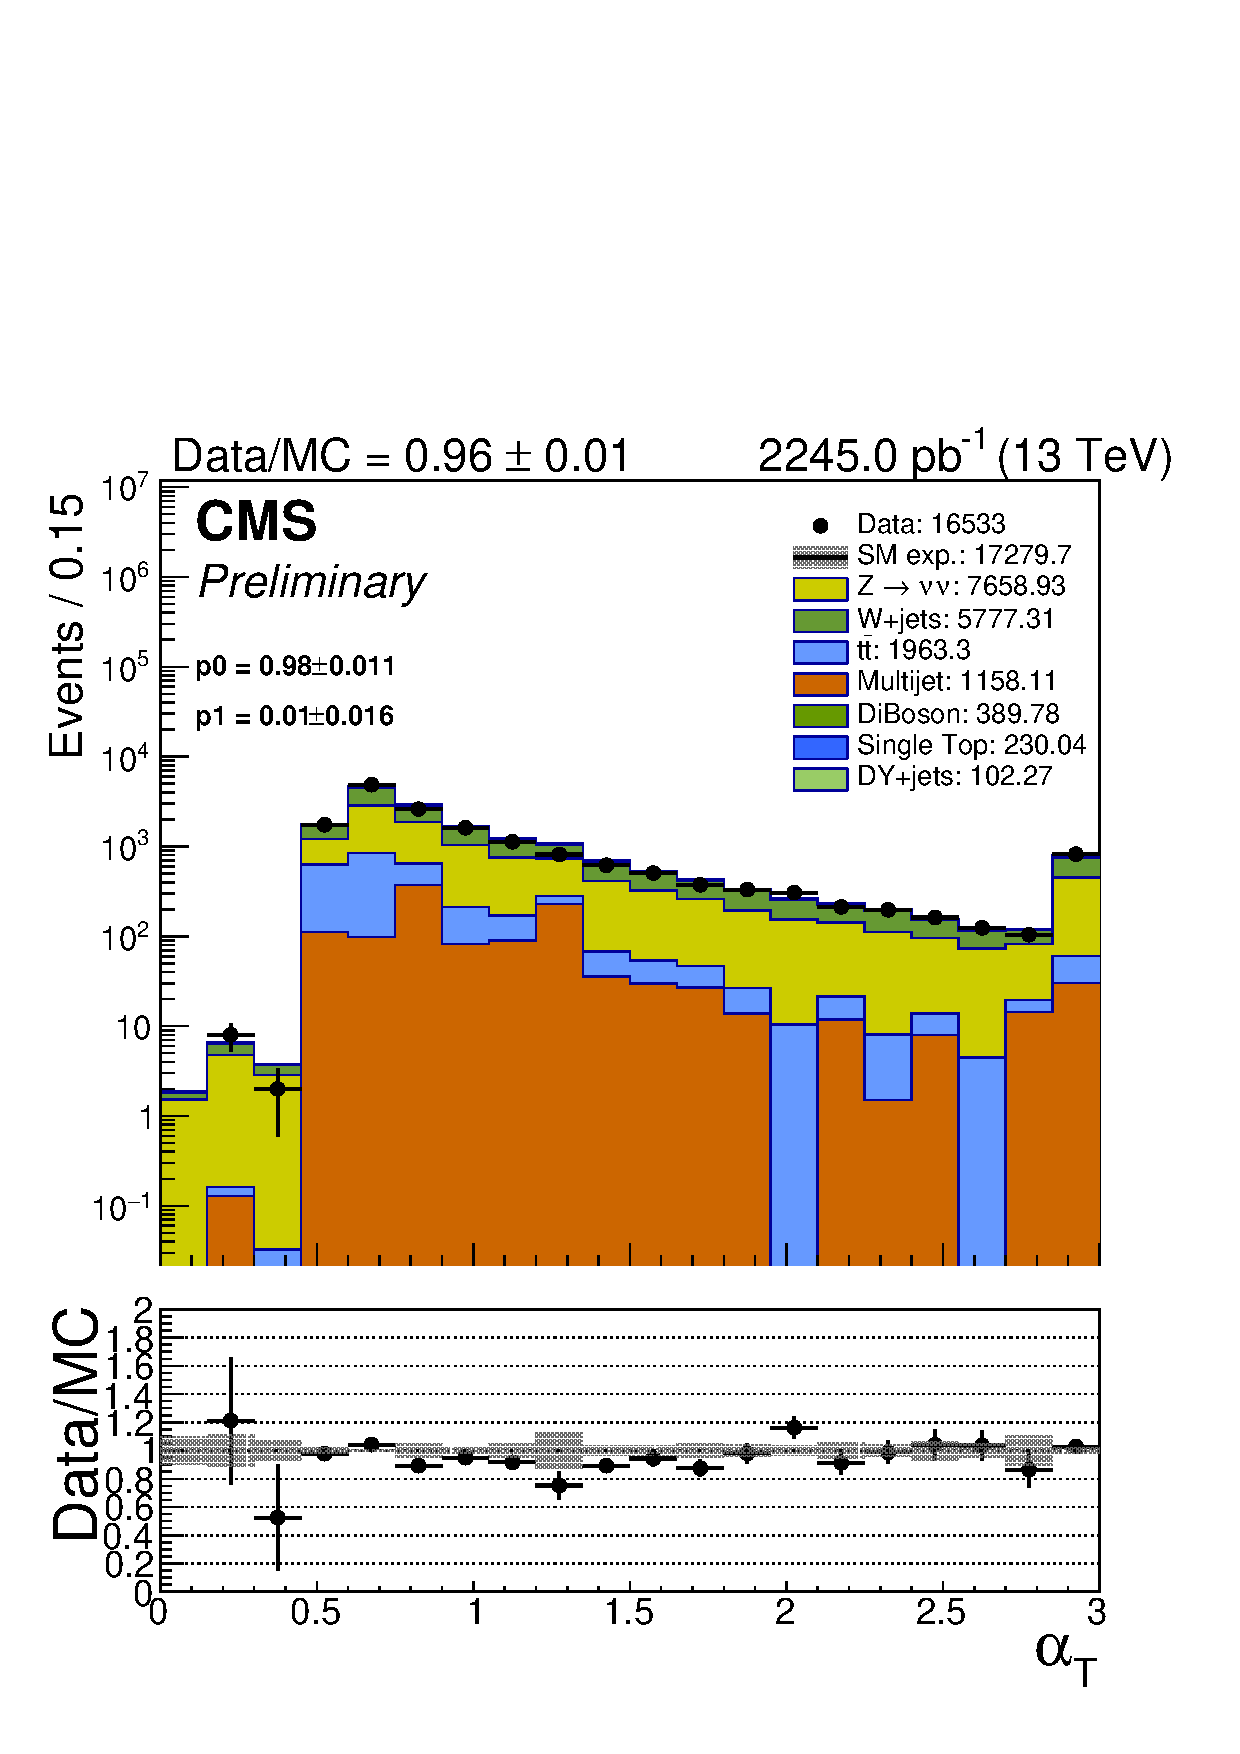
\includegraphics[width=0.38\textwidth]{figures/correctedShapes/asym/all/alphaT_asym_all}}\\
%%         \caption{The \mht distribution comparing data and prediction agreement before and after applying the correction from the control region only fit. Also shown are the results of a linear fit to the data/prediction ratio (p0,p1 parameters) which confirms the agreeement is significantly improved through the correction applied in the control regions}
%%     \end{center}
%% \end{figure}
%% \begin{figure}[tbhp]
%%     \begin{center}
%%         \subfigure[Symmetric Uncorrected]{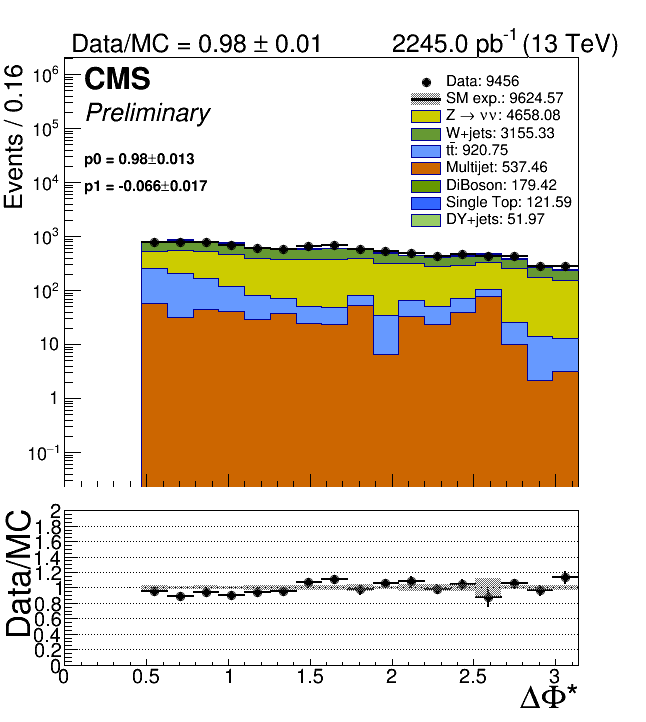
\includegraphics[width=0.38\textwidth]{figures/uncorrectedShapes/sym/all/biasedDPhi_sym_all}} ~~
%%         \subfigure[Symmetric Corrected] {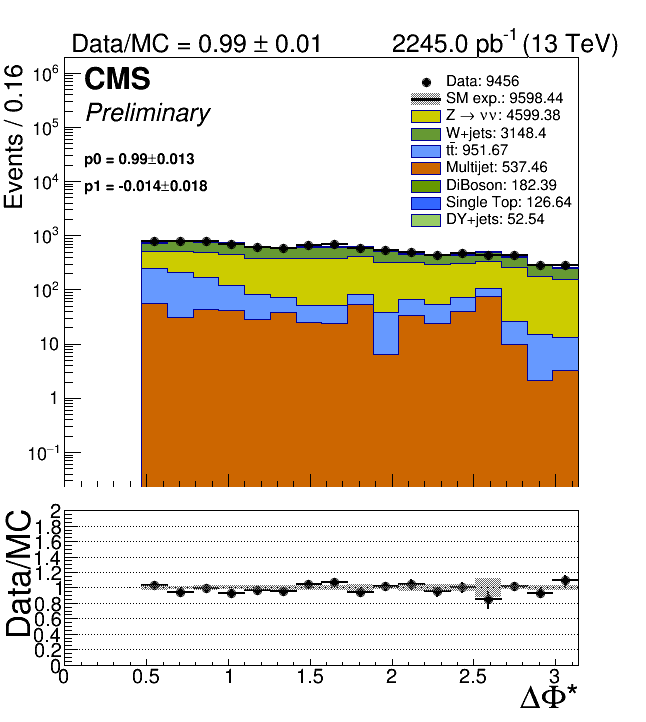
\includegraphics[width=0.38\textwidth]{figures/correctedShapes/sym/all/biasedDPhi_sym_all}}\\
%%         \subfigure[Asymmetric Uncorrected] {\includegraphics[width=0.38\textwidth]{figures/uncorrectedShapes/asym/all/biasedDPhi_asym_all}} ~~
%%         \subfigure[Asymmetric Corrected] {\includegraphics[width=0.38\textwidth]{figures/correctedShapes/asym/all/biasedDPhi_asym_all}}\\
%%         \subfigure[Monojet Unorrected] {\includegraphics[width=0.38\textwidth]{figures/uncorrectedShapes/mono/all/biasedDPhi20_mono_all}} ~~
%%         \subfigure[Monojet Corrected]{\includegraphics[width=0.38\textwidth]{figures/correctedShapes/mono/all/biasedDPhi20_mono_all}}\\
%%         \caption{The \bdphi distribution (including jets down to \pt = 20 GeV for monojet) comparing data and prediction agreement before and after applying the correction from the control region only fit. Also shown are the results of a linear fit to the data/prediction ratio (p0,p1 parameters) which confirms the agreeement is significantly improved through the correction applied in the control regions}
%%     \end{center}
%% \end{figure}
%% \begin{figure}[tbhp]
%%     \begin{center}
%%         \subfigure[Symmetric uncorrected]{\includegraphics[width=0.38\textwidth]{figures/uncorrectedShapes/sym/all/jet_pt[0]_sym_all}} ~~
%%         \subfigure[Symmetric corrected] {\includegraphics[width=0.38\textwidth]{figures/correctedShapes/sym/all/jet_pt[0]_sym_all}}\\
%%         \subfigure[Asymmetric uncorrected] {\includegraphics[width=0.38\textwidth]{figures/uncorrectedShapes/asym/all/jet_pt[0]_asym_all}} ~~
%%         \subfigure[Asymmetric corrected] {\includegraphics[width=0.38\textwidth]{figures/correctedShapes/asym/all/jet_pt[0]_asym_all}}\\
%%         \subfigure[Monojet uncorrected] {\includegraphics[width=0.38\textwidth]{figures/uncorrectedShapes/mono/all/jet_pt[0]_mono_all}} ~~
%%         \subfigure[Monojet corrected]{\includegraphics[width=0.38\textwidth]{figures/correctedShapes/mono/all/jet_pt[0]_mono_all}}\\
%%         \caption{The \bdphi distribution comparing data and prediction agreement before and after applying the correction from the control region only fit. Also shown are the results of a linear fit to the data/prediction ratio (p0,p1 parameters) which confirms the agreeement is significantly improved through the correction applied in the control regions}
%%     \end{center}
%% \end{figure}
%% \begin{figure}[tbhp]
%%     \begin{center}
%%         \subfigure[Symmetric Uncorrected]{\includegraphics[width=0.38\textwidth]{figures/uncorrectedShapes/sym/all/jet_pt[2]_sym_all}} ~~
%%         \subfigure[Symmetric Corrected] {\includegraphics[width=0.38\textwidth]{figures/correctedShapes/sym/all/jet_pt[2]_sym_all}}\\
%%         \subfigure[Asymmetric Uncorrected] {\includegraphics[width=0.38\textwidth]{figures/uncorrectedShapes/asym/all/jet_pt[2]_asym_all}} ~~
%%         \subfigure[Asymmetric Corrected] {\includegraphics[width=0.38\textwidth]{figures/correctedShapes/asym/all/jet_pt[2]_asym_all}}\\
%%         \caption{The third jet \pt distribution comparing data and prediction agreement before and after applying the correction from the control region only fit. Also shown are the results of a linear fit to the data/prediction ratio (p0,p1 parameters) which confirms the agreeement is significantly improved through the correction applied in the control regions}
%%     \end{center}
%% \end{figure}
%% \begin{figure}[tbhp]
%%     \begin{center}
%%         \subfigure[Symmetric uncorrected]{\includegraphics[width=0.38\textwidth]{figures/uncorrectedShapes/sym/all/nJet40_sym_all}} ~~
%%         \subfigure[Symmetric corrected] {\includegraphics[width=0.38\textwidth]{figures/correctedShapes/sym/all/nJet40_sym_all}}\\
%%         \subfigure[Asymmetric uncorrected] {\includegraphics[width=0.38\textwidth]{figures/uncorrectedShapes/asym/all/nJet40_asym_all}} ~~
%%         \subfigure[Asymmetric corrected] {\includegraphics[width=0.38\textwidth]{figures/correctedShapes/asym/all/nJet40_asym_all}}\\
%%         \caption{The \njet distribution comparing data and prediction agreement before and after applying the correction from the control region only fit. Also shown are the results of a linear fit to the data/prediction ratio (p0,p1 parameters) which confirms the agreeement is significantly improved through the correction applied in the control regions}
%%     \end{center}
%% \end{figure}
%% \begin{figure}[tbhp]
%%     \begin{center}
%%         \subfigure[Symmetric uncorrected]{\includegraphics[width=0.38\textwidth]{figures/uncorrectedShapes/sym/all/nBJet40_sym_all}} ~~
%%         \subfigure[Symmetric corrected] {\includegraphics[width=0.38\textwidth]{figures/correctedShapes/sym/all/nBJet40_sym_all}}\\
%%         \subfigure[Asymmetric uncorrected] {\includegraphics[width=0.38\textwidth]{figures/uncorrectedShapes/asym/all/nBJet40_asym_all}} ~~
%%         \subfigure[Asymmetric corrected] {\includegraphics[width=0.38\textwidth]{figures/correctedShapes/asym/all/nBJet40_asym_all}}\\
%%         \subfigure[Monojet uncorrected] {\includegraphics[width=0.38\textwidth]{figures/uncorrectedShapes/mono/all/nBJet40_mono_all}} ~~
%%         \subfigure[Monojet corrected]{\includegraphics[width=0.38\textwidth]{figures/correctedShapes/mono/all/nBJet40_mono_all}}\\
%%         \caption{The \nb distribution comparing data and prediction agreement before and after applying the correction from the control region only fit. Also shown are the results of a linear fit to the data/prediction ratio (p0,p1 parameters) which confirms the agreeement is significantly improved through the correction applied in the control regions}
%%         \label{fig:shapesbjet}
%%     \end{center}
%% \end{figure}
